%%%%%%%%%%%%%%%%%%%%%%%%%%%%%%%%%%%%%%%%%%%%%%%%%%%%%%%%%%%%%%%%%%%%%%%%%%%%%%%
%                       CARREGA DE LA CLASSE DE DOCUMENT                      %
%                                                                             %
% Les opcions admissibles son:                                                %
%      12pt / 11pt            (cos dels tipus de lletra; no feu servir 10pt)  %
%                                                                             %
% catalan/spanish/english     (llengua principal del treball)                 %
%                                                                             % 
% french/italian/german...    (si necessiteu fer servir alguna altra llengua) %
%                                                                             %
% listoffigures               (El document inclou un Index de figures)        %
% listoftables                (El document inclou un Index de taules)         %
% listofquadres               (El document inclou un Index de quadres)        %
% listofalgorithms            (El document inclou un Index d'algorismes)      %
%                                                                             %
%%%%%%%%%%%%%%%%%%%%%%%%%%%%%%%%%%%%%%%%%%%%%%%%%%%%%%%%%%%%%%%%%%%%%%%%%%%%%%%

\documentclass[11pt,spanish,listoffigures,listoftables]{tfgetsinf}


\usepackage{pgfplotstable} % Para leer y mostrar tablas desde CSV
\usepackage{booktabs}       % Para mejorar el diseño de la tabla
\usepackage{multirow}       % Para fusionar filas
\usepackage{caption}
\usepackage{subcaption}


\usepackage{float}          % Para usar [H] en las figuras
\usepackage{amsmath}        % Para usar \text en modo matemático
\usepackage{tabularx}       % Para usar el entorno tabularx
\usepackage{array}          % Para usar >{} en las columnas de la tabla
%%%%%%%%%%%%%%%%%%%%%%%%%%%%%%%%%%%%%%%%%%%%%%%%%%%%%%%%%%%%%%%%%%%%%%%%%%%%%%%
%                     CODIFICACIO DEL FITXER FONT                             %
%                                                                             %
%    windows fa servir normalment 'ansinew'                                   %
%    amb linux es possible que siga 'latin1' o 'latin9'                       %s
%    Pero el mes recomanable es fer servir utf8 (unicode 8)                   %
%                                          (si el vostre editor ho permet)    % 
%%%%%%%%%%%%%%%%%%%%%%%%%%%%%%%%%%%%%%%%%%%%%%%%%%%%%%%%%%%%%%%%%%%%%%%%%%%%%%%

\usepackage[utf8]{inputenc} 
%%%%%%%%%%%%%%%%%%%%%%%%%%%%%%%%%%%%%%%%%%%%%%%%%%%%%%%%%%%%%%%%%%%%%
% Para conseguir que la tabla de contenido no salga en rojo
%%%%%%%%%%%%%%%%%%%%%%%%%%%%%%%%%%%%%%%%%%%%%%%%%%%%%%%%%%%%%%%%%%%%%

\usepackage[acronym]{glossaries}
\makeglossaries

\hypersetup{ colorlinks=true, linkcolor=black, urlcolor=cyan, }


\newacronym[plural={AIs}, firstplural={Inteligencias Artificiales (AIs)}]{ai}{AI}{Inteligencia Artificial}
\newacronym[plural={CNNs}, firstplural={Redes Neuronales Convolucionales (CNNs)}]{cnn}{CNN}{Red Neuronal Convolucional}
\newacronym[plural={CPUs}, firstplural={Unidades Centrales de Procesamiento (CPUs)}]{cpu}{CPU}{Unidad Central de Procesamiento}
\newacronym[plural={GPUs}, firstplural={Unidades de Procesamiento Gráfico (GPUs)}]{gpu}{GPU}{Unidad de Procesamiento Gráfico}
\newacronym[plural={DLAs}, firstplural={Aceleradores de Aprendizaje Profundo (DLAs)}]{dla}{DLA}{Acelerador de Aprendizaje Profundo}
\newacronym[plural={TPUs}, firstplural={Unidades de Procesamiento Tensorial (TPUs)}]{tpu}{TPU}{Unidad de Procesamiento Tensorial}
\newacronym[plural={FPS}]{fps}{FPS}{Frames Por Segundo} % FPS suele ser invariable en plural
\newacronym[plural={IoUs}]{iou}{IoU}{Intersection over Union}
\newacronym[plural={mAPs}]{map}{mAP}{mean Average Precision}
\newacronym[plural={MOTs}]{mot}{MOT}{Multiple Object Tracking}
\newacronym[plural={MOTAs}]{mota}{MOTA}{Multiple Object Tracking Accuracy}
\newacronym[plural={MOTPs}]{motp}{MOTP}{Multiple Object Tracking Precision}
\newacronym[plural={NMS}]{nms}{NMS}{Non-Maximum Suppression} % NMS suele ser invariable
\newacronym[plural={SSDs}]{ssd}{SSD}{Single Shot MultiBox Detector}
\newacronym[plural={YOLOs}]{yolo}{YOLO}{You Only Look Once}
\newacronym[plural={GILs}]{gil}{GIL}{Global Interpreter Lock}
\newacronym[plural={SIMTs}]{simt}{SIMT}{Single Instruction Multiple Threads}
\newacronym[plural={ASICs}]{asic}{ASIC}{Application-Specific Integrated Circuit}
\newacronym[plural={FPGAs}]{fpga}{FPGA}{Field Programmable Gate Array}
\newacronym[plural={SDKs}]{sdk}{SDK}{Software Development Kit}
\newacronym[plural={MLPs}]{mlp}{MLP}{Multilayer Perceptron}
\newacronym[plural={HOGs}]{hog}{HOG}{Histogram of Oriented Gradients}
\newacronym[plural={R-CNNs}]{rcnn}{R-CNN}{Region-based Convolutional Neural Network}
\newacronym{gap}{GAP}{Grupo de Arquitecturas Paralelas}
\newacronym{upv}{UPV}{Universidad Politécnica de Valencia}
\newacronym{sdl}{SDL}{Sistemas Basados en Deep Learning para la Industria}
\newacronym{onnx}{ONNX}{Open Neural Network Exchange}




%%%%%%%%%%%%%%%%%%%%%%%%%%%%%%%%%%%%%%%%%%%%%%%%%%%%%%%%%%%%%%%%%%%%%%%%%%%%%%%
%                        ALTRES PAQUETS I DEFINICIONS                         %
%                                                                             %
% Carregueu aci els paquets que necessiteu i declareu les comandes i entorns  %
%                                          (aquesta seccio pot ser buida)     %
%%%%%%%%%%%%%%%%%%%%%%%%%%%%%%%%%%%%%%%%%%%%%%%%%%%%%%%%%%%%%%%%%%%%%%%%%%%%%%%



%%%%%%%%%%%%%%%%%%%%%%%%%%%%%%%%%%%%%%%%%%%%%%%%%%%%%%%%%%%%%%%%%%%%%%%%%%%%%%%
%                        DADES DEL TREBALL                                    %
%                                                                             %
% titol, alumne, tutor i curs academic                                        %
%%%%%%%%%%%%%%%%%%%%%%%%%%%%%%%%%%%%%%%%%%%%%%%%%%%%%%%%%%%%%%%%%%%%%%%%%%%%%%%

\title{Detección de defectos en objetos en movimiento mediante Redes Neuronales Convolucionales con optimizaciones específicas para hardware NVIDIA}
\author{Haro Armero, Abel}
\tutor{Flich Cardo, José \\
López Rodríguez, Pedro Juan}
\curs{2024-2025}

%%%%%%%%%%%%%%%%%%%%%%%%%%%%%%%%%%%%%%%%%%%%%%%%%%%%%%%%%%%%%%%%%%%%%%%%%%%%%%%
%                     PARAULES CLAU/PALABRAS CLAVE/KEY WORDS                  %
%                                                                             %
% Independentment de la llengua del treball, s'hi han d'incloure              %
% les paraules clau i el resum en els tres idiomes                            %
%%%%%%%%%%%%%%%%%%%%%%%%%%%%%%%%%%%%%%%%%%%%%%%%%%%%%%%%%%%%%%%%%%%%%%%%%%%%%%%

\keywords{Xarxes Neuronals Convolucionals, Detecció de defectes, Visió per computador, NVIDIA Jetson, Temps real, Optimització energètica}
   {Redes Neuronales Convolucionales, Detección de defectos, Visión por computador, NVIDIA Jetson, Tiempo real, Optimización energética}
   {Convolutional Neural Networks, Defect Detection, Computer Vision, NVIDIA Jetson, Real-Time, Energy Optimization}

%%%%%%%%%%%%%%%%%%%%%%%%%%%%%%%%%%%%%%%%%%%%%%%%%%%%%%%%%%%%%%%%%%%%%%%%%%%%%%%
%                              INICI DEL DOCUMENT                             %
%%%%%%%%%%%%%%%%%%%%%%%%%%%%%%%%%%%%%%%%%%%%%%%%%%%%%%%%%%%%%%%%%%%%%%%%%%%%%%%

\begin{document}

%%%%%%%%%%%%%%%%%%%%%%%%%%%%%%%%%%%%%%%%%%%%%%%%%%%%%%%%%%%%%%%%%%%%%%%%%%%%%%%
%              RESUMS DEL TFG EN VALENCIA, CASTELLA I ANGLES                  %
%%%%%%%%%%%%%%%%%%%%%%%%%%%%%%%%%%%%%%%%%%%%%%%%%%%%%%%%%%%%%%%%%%%%%%%%%%%%%%%

\begin{abstract}
Aquest treball de fi de grau aborda el desafiament de la detecció automàtica de defectes en objectes que es desplacen en entorns industrials, com ara línies de producció. Es presenta el disseny i la implementació d'un sistema complet de visió artificial basat en tècniques d'aprenentatge profund.

El nucli del sistema és un model de xarxa neuronal convolucional (CNN), específicament una variant optimitzada de l'arquitectura YOLO, entrenat per identificar i localitzar amb precisió diversos tipus de defectes en temps real. Per fer front a les restriccions computacionals i energètiques pròpies dels sistemes encastats, el model s'ha implementat sobre acceleradors hardware de baix consum de la sèrie NVIDIA Jetson. S'han aplicat tècniques avançades d'optimització, incloent la conversió a TensorRT i l'exploració de diferents precisions numèriques, per maximitzar la velocitat d'inferència (FPS) i minimitzar el consum energètic (Watts) sense comprometre significativament la precisió de la detecció (mAP). 

El treball inclou una anàlisi exhaustiva del rendiment del sistema sota diverses configuracions de hardware i software, demostrant la viabilitat d'aplicar solucions d'intel·ligència artificial d'alt rendiment en escenaris industrials amb recursos limitats.
\end{abstract}

\begin{abstract}[spanish]
Este trabajo de fin de grado aborda el desafío de la detección automática de defectos en objetos que se desplazan en entornos industriales, como líneas de producción. Se presenta el diseño y la implementación de un sistema completo de visión artificial basado en técnicas de aprendizaje profundo.

El núcleo del sistema es un modelo de red neuronal convolucional (CNN), específicamente una variante optimizada de la arquitectura YOLO, entrenado para identificar y localizar con precisión diversos tipos de defectos en tiempo real. Para hacer frente a las restricciones computacionales y energéticas propias de los sistemas embebidos, el modelo se ha implementado sobre aceleradores hardware de bajo consumo de la serie NVIDIA Jetson. Se han aplicado técnicas avanzadas de optimización, incluyendo la conversión a TensorRT y la exploración de diferentes precisiones numéricas, para maximizar la velocidad de inferencia (FPS) y minimizar el consumo energético (Watts) sin comprometer significativamente la precisión de la detección (mAP).

El trabajo incluye un análisis exhaustivo del rendimiento del sistema bajo diversas configuraciones de hardware y software, demostrando la viabilidad de aplicar soluciones de inteligencia artificial de alto rendimiento en escenarios industriales con recursos limitados.
\end{abstract}
\begin{abstract}[english]
This bachelor's thesis addresses the challenge of automatic defect detection in moving objects within industrial environments, such as production lines. It presents the design and implementation of a complete computer vision system based on deep learning techniques.

The core of the system is a convolutional neural network (CNN) model, specifically an optimized variant of the YOLO architecture, trained to accurately identify and locate various types of defects in real-time. To address the computational and energy constraints inherent in embedded systems, the model has been implemented on low-power hardware accelerators from the NVIDIA Jetson series. Advanced optimization techniques have been applied, including conversion to TensorRT and exploration of different numerical precisions, to maximize inference speed (FPS) and minimize energy consumption (Watts) without significantly compromising detection accuracy (mAP).

The work includes a comprehensive analysis of the system's performance under various hardware and software configurations, demonstrating the feasibility of applying high-performance artificial intelligence solutions in industrial scenarios with limited resources.
\end{abstract}

%%%%%%%%%%%%%%%%%%%%%%%%%%%%%%%%%%%%%%%%%%%%%%%%%%%%%%%%%%%%%%%%%%%%%%%%%%%%%%%
%                              CONTINGUT DEL TREBALL                          %
%%%%%%%%%%%%%%%%%%%%%%%%%%%%%%%%%%%%%%%%%%%%%%%%%%%%%%%%%%%%%%%%%%%%%%%%%%%%%%%

\mainmatter

%%%%%%%%%%%%%%%%%%%%%%%%%%%%%%%%%%%%%%%%%%%%%%%%%%%%%%%%%%%%%%%%%%%%%%%%%%%%%%%
%                                  INTRODUCCIO                                %
%%%%%%%%%%%%%%%%%%%%%%%%%%%%%%%%%%%%%%%%%%%%%%%%%%%%%%%%%%%%%%%%%%%%%%%%%%%%%%%

\chapter{Introducci\'on}\label{chap:introduccion}
Durante los últimos años, la inteligencia artificial ha experimentado un crecimiento en popularidad sin precedentes, transformando nuestra capacidad tecnológica con herramientas revolucionarias. Este avance ha sido impulsado por la disponibilidad de grandes volúmenes de datos, el desarrollo de algoritmos avanzados y las mejoras significativas en el hardware de procesamiento, que han permitido a las máquinas aprender y adaptarse a situaciones complejas. Algunos campos destacados de aplicación incluyen el procesamiento del lenguaje natural, la visión por computador y la robótica. En particular, la visión por computador ha visto un auge significativo, con aplicaciones en áreas como la seguridad, la medicina y la automoción. Esta creciente popularidad por el mundo de la inteligencia artificial se refleja en la evolución del interés público en ella, como muestra la Figura~\ref{fig:interes_en_inteligencia_artificial}.

\begin{figure}[H]
   \centering
   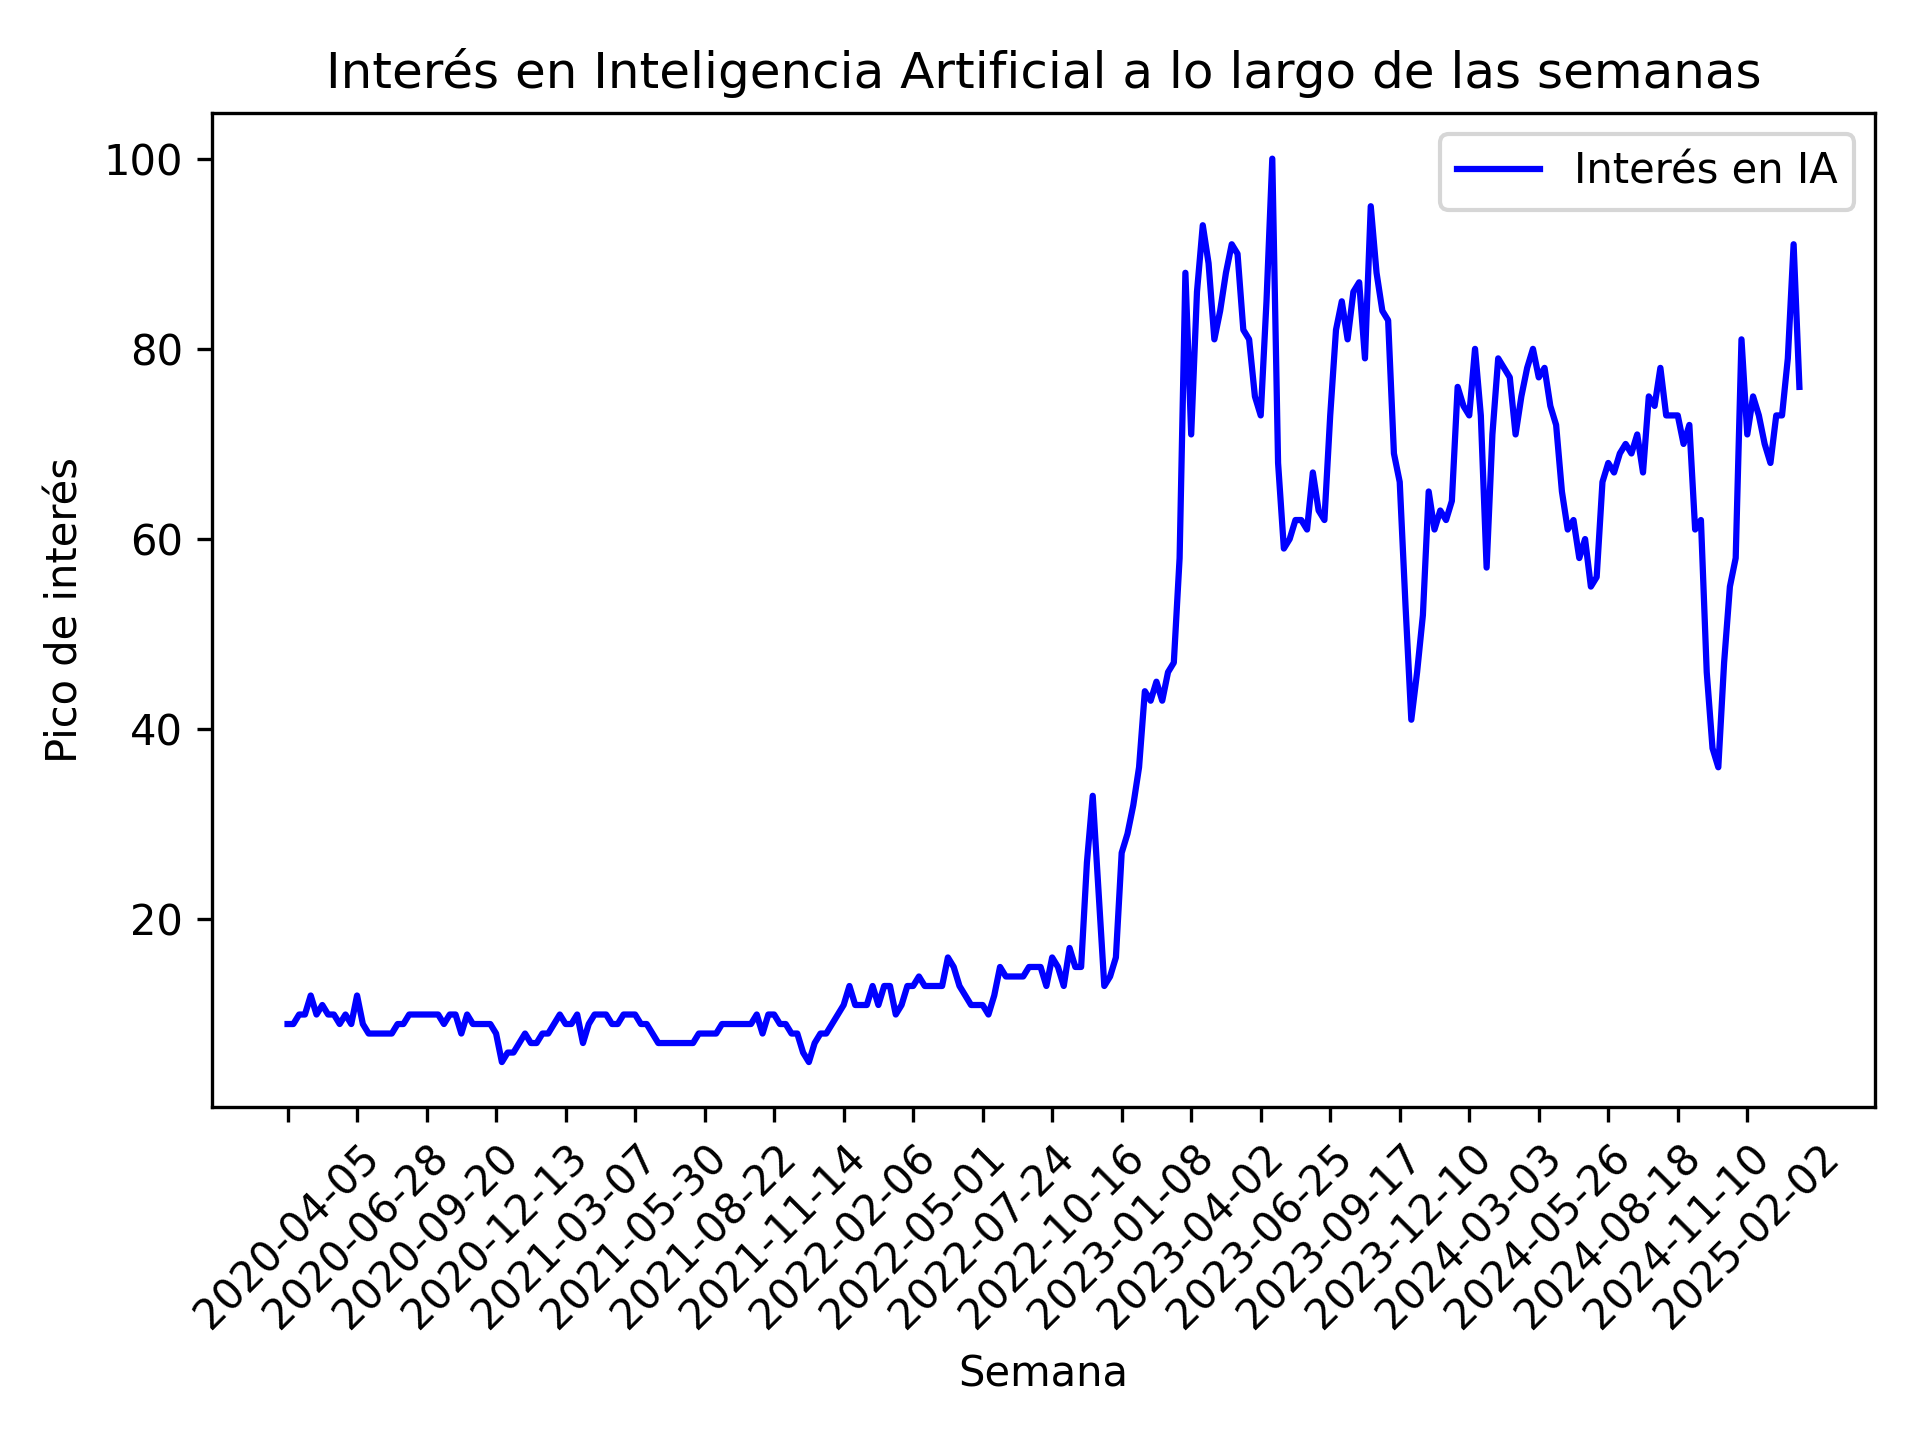
\includegraphics[width=0.7\textwidth]{excels/introduccion/interes_en_ia.png}
   \caption{Evolución del interés público en inteligencia artificial según datos de Google Trends (2020-2025).}
\label{fig:interes_en_inteligencia_artificial}
\end{figure}

El progreso en visión por computador ha sido posible gracias a los avances en redes neuronales convolucionales, que han revolucionado la capacidad de los sistemas para detectar y clasificar objetos en imágenes y vídeos con una gran precisión y velocidad.

Estos algoritmos de visión artificial requieren una potencia computacional significativa tanto para su entrenamiento como para su ejecución. Las \glspl{cpu} tradicionales resultan insuficientes para estas tareas, por lo que la industria ha desarrollado arquitecturas específicas como las \glspl{gpu}\cite[cap. ~3, pp. ~2-7]{hwu2022programming}, \glspl{tpu}\cite{google2025tpu} y \glspl{dla}\cite{nvidia_dla}. Estos componentes están optimizados para ejecutar operaciones de entrenamiento e inferencia de manera eficiente, permitiendo implementar sistemas de visión artificial capaces de procesar información visual en tiempo real. Sin embargo, estos aceleradores suelen presentar un consumo energético elevado, lo que plantea importantes retos de eficiencia y sostenibilidad.



\begin{figure}[H]
   \centering
   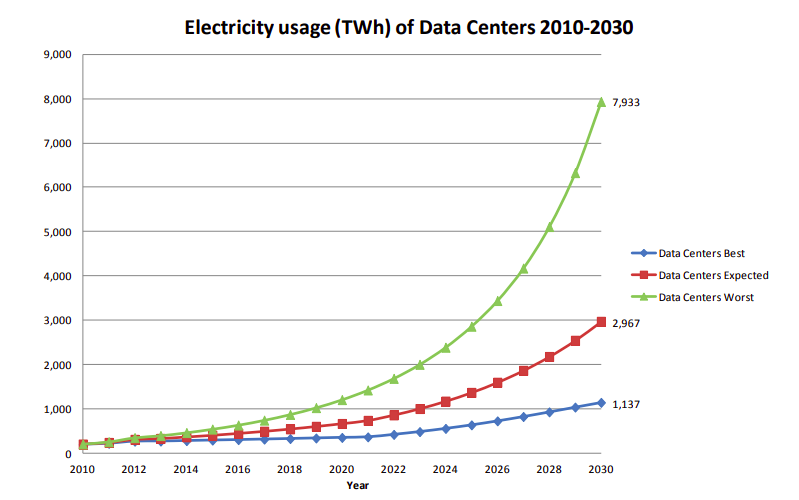
\includegraphics[width=0.7\textwidth]{images/introduccion/consumo_electrico_datacenters.png}
   \caption[Proyección del consumo eléctrico de los centros de datos en el mundo]{Proyección del consumo eléctrico de los centros de datos en el mundo. Extraído de \cite[fig. 4, p. ~17]{challe6010117}.}
\label{fig:consumo_electrico_datacenters}
\end{figure}

Como se observa en la Figura~\ref{fig:consumo_electrico_datacenters}, el consumo eléctrico de los centros de datos en el mundo ha ido aumentando de forma exponencial, lo que plantea un desafío significativo para la sostenibilidad del crecimiento tecnológico \cite{challe6010117}. En el peor escenario, esta tendencia podría llevar a un incremento insostenible en la huella de carbono del sector tecnológico, mientras que en el mejor de los casos, la adopción de tecnologías eficientes podría moderar el crecimiento. Este aumento del consumo energético no solo afecta a los centros de datos, sino también a los dispositivos embebidos y móviles, donde la eficiencia energética es crucial para prolongar la vida útil de las baterías y reducir el impacto ambiental.

Para enfrentar estos desafíos, se han desarrollado diversas técnicas de optimización y compresión que reducen el tamaño y la complejidad de los modelos neuronales manteniendo su rendimiento. Paralelamente, han surgido arquitecturas hardware específicamente diseñadas para la inferencia de modelos de aprendizaje profundo en entornos con restricciones energéticas. En este contexto, los dispositivos de la serie Jetson de NVIDIA\cite{nvidia_jetson_modules} destacan por ofrecer un equilibrio entre alto rendimiento en tareas de inteligencia artificial y un consumo energético contenido, ideal para aplicaciones embebidas de visión artificial.

La combinación de redes neuronales convolucionales y aceleradores hardware ha permitido la creación de sistemas de visión artificial que pueden detectar y clasificar objetos en movimiento, lo que es esencial en aplicaciones como la vigilancia, la conducción autónoma y la robótica.

Con todo ello en mente, este trabajo se centra en el desarrollo de un sistema de visión artificial capaz de detectar y clasificar objetos con posibles defectos en movimiento, utilizando redes neuronales convolucionales y aceleradores hardware de bajo consumo. 

\begin{figure}[H]
   \centering
   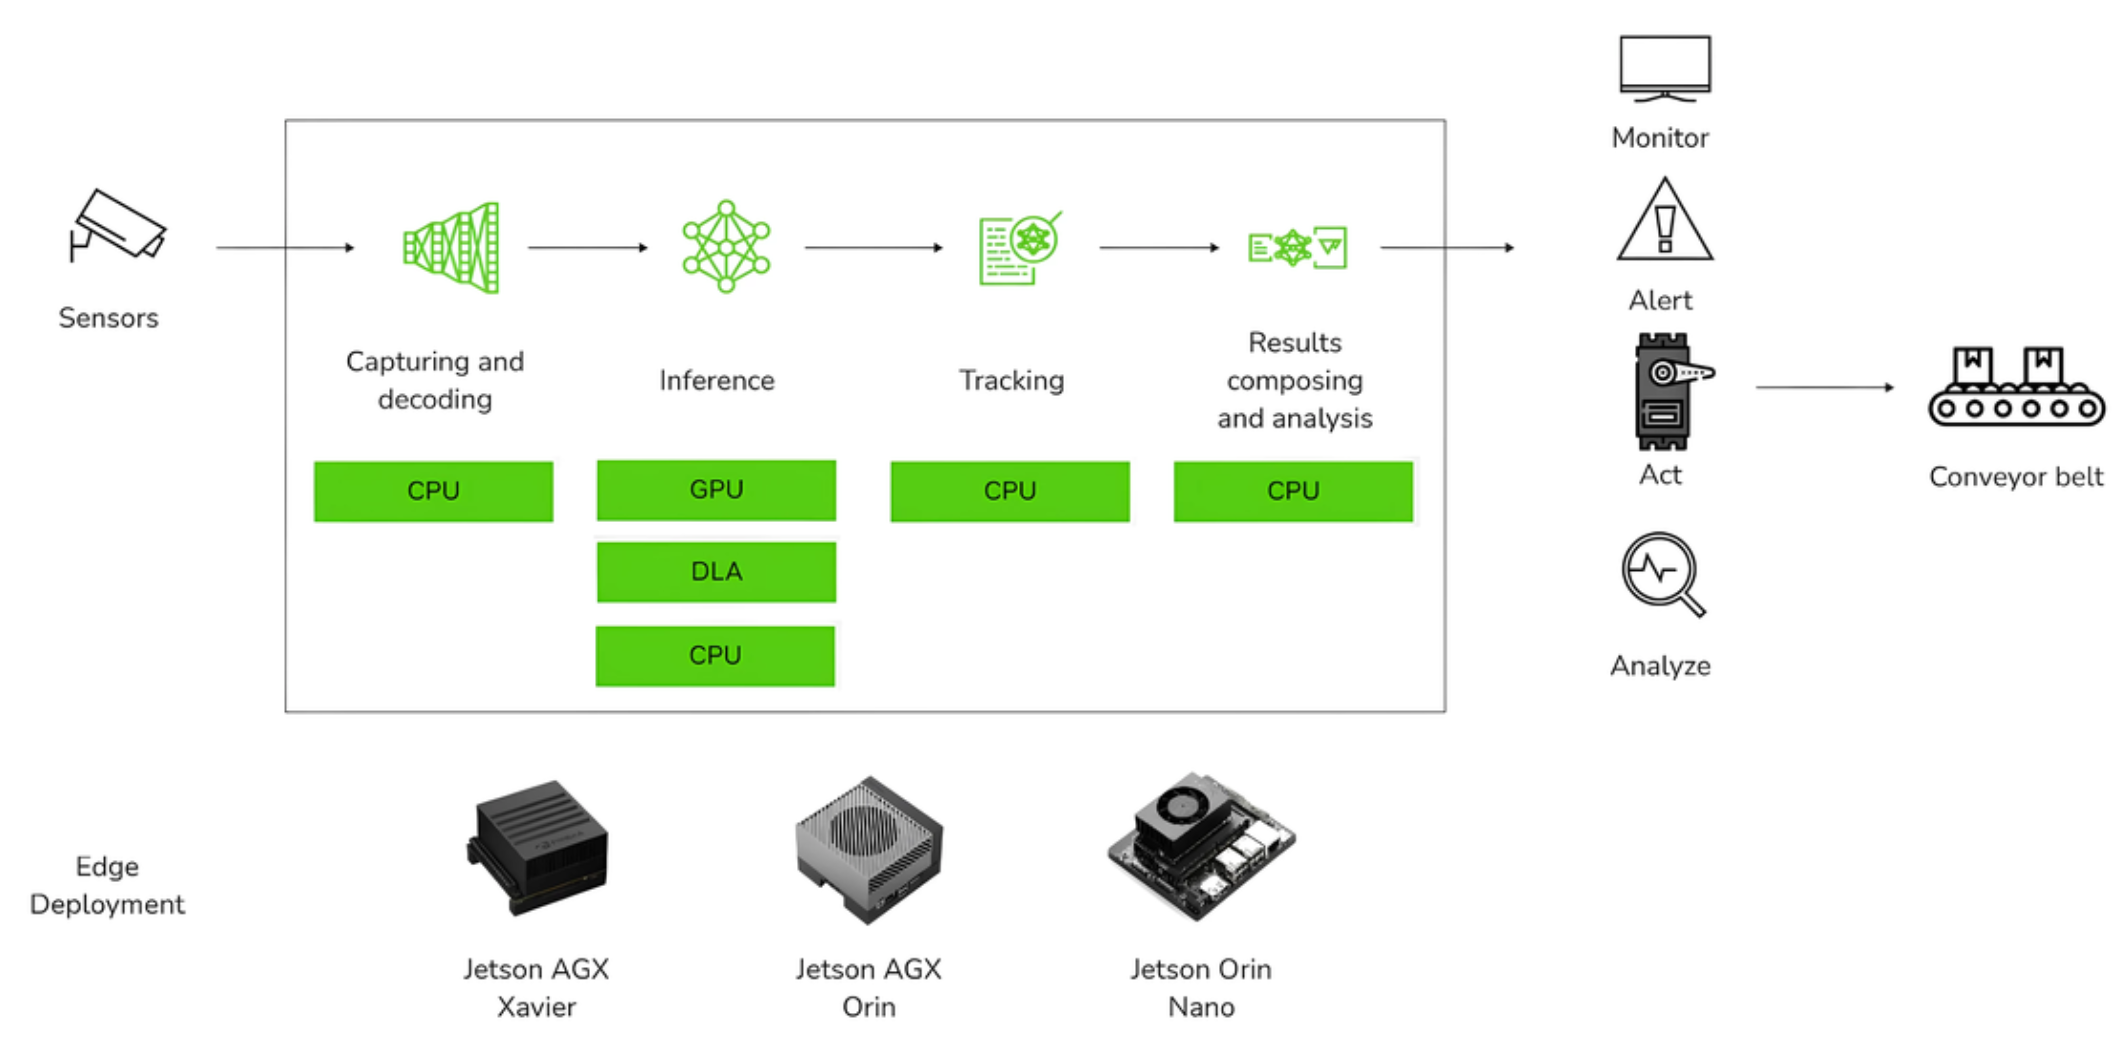
\includegraphics[width=0.7\textwidth]{images/diseno_e_implementacion/figura_TFG_v3.png}
   \caption{Esquema del sistema de visión artificial propuesto.}
\label{fig:esquema_TFG}
\end{figure}

La Figura~\ref{fig:esquema_TFG} ilustra el esquema del sistema de visión artificial propuesto. Este sistema se basa en la captura de imágenes de objetos en movimiento, que son procesadas por un modelo de red neuronal convolucional (CNN) para detectar y clasificar posibles defectos. El modelo se ejecuta en un dispositivo NVIDIA Jetson, optimizado para ofrecer un rendimiento eficiente en términos de velocidad y consumo energético. La implementación del sistema incluye la captura y etiquetado de imágenes, el diseño y entrenamiento del modelo CNN, así como la integración con el hardware NVIDIA para su despliegue en entornos industriales.

\section{Motivaci\'on}\label{sec:motivacion}

Los humanos somos capaces de ver y entender el mundo que nos rodea. Dada una imagen, podemos identificar objetos, reconocer patrones y tomar decisiones basadas en la información visual. Sin embargo, esta capacidad no es innata en las máquinas. La visión por computador es la ciencia que busca dotar a las máquinas de la capacidad de interpretar y comprender imágenes y vídeos, emulando la forma en que los humanos percibimos el entorno.

Como se mencionó anteriormente, la inteligencia artificial ha revolucionado la forma en que interactuamos con la tecnología. Se ha convertido en una herramienta esencial para aplicar soluciones innovadoras en una amplia gama de campos. En particular, la visión por computador ha demostrado ser un área de gran potencial. También la existencia de dispositivos de bajo consumo, como los de la serie Jetson de NVIDIA, ha permitido llevar la inteligencia artificial a entornos de edge computing (cómputo en el borde), donde se acerca el procesamiento de datos a la fuente de información. Esto reduce la latencia y el consumo energético. Con todo esto, se abre un abanico de posibilidades para la implementación de sistemas de visión artificial en aplicaciones industriales.

Centrándose en el ámbito industrial, la detección y clasificación de objetos en movimiento es crucial para optimizar procesos, mejorar la seguridad y aumentar la eficiencia. En la mayoría de los entornos productivos, la detección de defectos se realiza de forma manual, lo que puede ser ineficiente y propenso a errores. La automatización de este proceso mediante sistemas de visión artificial puede reducir costes, aumentar la precisión y mejorar la calidad del producto final.


La motivación de este trabajo radica en la necesidad de desarrollar un sistema de visión artificial capaz de detectar y clasificar objetos en movimiento en un entorno industrial, específicamente en una cinta transportadora.


\section{Objetivos}\label{sec:objetivos}

El objetivo principal de este trabajo es desarrollar un sistema de visión artificial capaz de detectar y clasificar objetos en movimiento en una cinta transportadora utilizando redes neuronales convolucionales y aceleradores hardware de bajo consumo. Para lograr este objetivo, se plantean los siguientes objetivos específicos:

\begin{itemize}
   \item Realizar un estudio del estado del arte en redes neuronales convolucionales, aceleradores hardware de bajo consumo y técnicas avanzadas de optimización para visión artificial.
   \item Desarrollar un conjunto de datos para el entrenamiento y evaluación del sistema, mediante la captura y etiquetado de imágenes de objetos en movimiento.
   \item Diseñar, entrenar y validar un modelo de red neuronal convolucional optimizado para la detección y clasificación en tiempo real de defectos en objetos en movimiento.
   \item Implementar un sistema completo de visión artificial que integre el modelo entrenado con los aceleradores hardware NVIDIA, enfocado en maximizar la eficiencia y minimizar la latencia.
   \item Analizar los cuellos de botella del sistema, y aplicar técnicas específicas de optimización para mejorar el rendimiento y la eficiencia energética.
   \item Cuantificar de manera exhaustiva el rendimiento del sistema mediante métricas precisas de exactitud (mAP, precisión, recall), latencia (FPS) y consumo energético (W, J/inferencia).
   \item Realizar un análisis comparativo sistemático entre diferentes configuraciones de hardware, software y parámetros de optimización para identificar la combinación que ofrezca el mejor equilibrio entre precisión, velocidad y eficiencia energética.
\end{itemize}

\section{Estructura de la memoria}\label{sec:estructura_memoria}

La memoria se estructura en seis capítulos, cada uno dedicado a un aspecto fundamental del trabajo desarrollado:

El \textbf{Capítulo~\ref{chap:introduccion}} introduce el proyecto, detallando la motivación subyacente, los objetivos específicos que se persiguen, la organización general de esta memoria y las colaboraciones para el desarrollo del trabajo.

El \textbf{Capítulo~\ref{chap:conceptos_previos}} sienta las bases teóricas del trabajo. Comienza explorando los fundamentos de la inteligencia artificial y avanza hacia los desarrollos más recientes en redes neuronales convolucionales aplicadas a la visión por computador. A continuación, se justifica el uso de aceleradores hardware para tareas de IA, presentando los dispositivos de bajo consumo NVIDIA Jetson. El capítulo concluye con una descripción de los algoritmos de seguimiento de objetos en tiempo real, detallando el funcionamiento de ByteTrack y las métricas de evaluación pertinentes.

El \textbf{Capítulo~\ref{chap:diseno_e_implementacion}} detalla el proceso de diseño e implementación del sistema de visión artificial. Se inicia con un análisis del problema, seguido de la descripción de la recolección de imágenes, su etiquetado y el entrenamiento de los modelos de detección. Concluye con el diseño modular del sistema, especificando sus etapas y las estrategias de segmentación consideradas para su implementación.

El \textbf{Capítulo~\ref{chap:evaluacion_solucion}} presenta la metodología empleada para evaluar el rendimiento del sistema. Define las métricas clave, describe la configuración de los experimentos y la recolección de datos. Posteriormente, se analizan exhaustivamente los resultados obtenidos, comparando el comportamiento del sistema bajo diversas configuraciones de hardware y software, y evaluando su precisión, velocidad y eficiencia energética.

El \textbf{Capítulo~\ref{chap:prueba_concepto}} describe la construcción de un prototipo de cinta transportadora, diseñado para validar el sistema de visión artificial en un entorno que simula condiciones de producción. Se presentan los resultados obtenidos durante esta prueba de concepto.

Finalmente, el \textbf{Capítulo~\ref{chap:conclusiones}} resume las principales conclusiones derivadas del trabajo, resaltando los logros alcanzados, las limitaciones identificadas y las posibles líneas de investigación y desarrollo futuras.

%\section{Notes bibliografiques} %%%%% Opcional

%????? ????????????? ????????????? ????????????? ????????????? ?????????????

%%%%%%%%%%%%%%%%%%%%%%%%%%%%%%%%%%%%%%%%%%%%%%%%%%%%%%%%%%%%%%%%%%%%%%%%%%%%%%%
%                         CAPITOLS (tants com calga)                          %
%%%%%%%%%%%%%%%%%%%%%%%%%%%%%%%%%%%%%%%%%%%%%%%%%%%%%%%%%%%%%%%%%%%%%%%%%%%%%%%

\section{Colaboraciones}

El presente Trabajo de Fin de Grado se ha desarrollado en el marco de una beca de colaboración y un periodo de prácticas de empresa, ambos focalizados en la investigación y desarrollo que sustenta este proyecto. Estas actividades se han llevado a cabo en el \gls{gap} de la \gls{upv}. El \gls{gap} es un grupo de investigación dentro de la universidad, que se dedica al diseño y evaluación de redes de interconexión para sistemas de computación paralela de altas prestaciones, tales como supercomputadores, clústeres y centros de datos. El Grupo de Arquitecturas Paralelas (GAP) de la Universidad Politécnica de Valencia cuenta con una amplia experiencia en el trabajo sobre redes de interconexión para computadoras paralelas, abarcando desde grandes supercomputadoras, pasando por clústeres de ordenadores personales, usualmente utilizados como servidores, hasta las redes en chip en procesadores multinúcleo. El GAP también ha desarrollado investigación en temas relacionados, como la microarquitectura de procesadores y los protocolos de coherencia de caché. Su investigación abarca también áreas como la optimización de arquitecturas para aplicaciones específicas y la mejora de la eficiencia energética en sistemas computacionales.

Esta colaboración se encuentra estrechamente vinculada con los contenidos y objetivos de la asignatura \gls{sdl}, una asignatura que forma parte de la mención de ingeniería dentro del Grado en Ingeniería Informática. La oportunidad de colaborar con el \gls{gap} ha permitido aplicar de manera práctica y en un contexto de investigación real los conocimientos teóricos y técnicos adquiridos durante la asignatura. Específicamente, ha facilitado la profundización en el diseño, implementación y optimización de sistemas de visión por computador basados en inteligencia artificial, enfrentando desafíos reales relacionados con el rendimiento, la eficiencia y el despliegue en hardware especializado. Esta sinergia entre la formación académica y la investigación aplicada ha enriquecido significativamente la experiencia de aprendizaje, fomentando el desarrollo de habilidades prácticas avanzadas y una comprensión más profunda de las complejidades inherentes al campo de la visión artificial y el aprendizaje profundo en entornos industriales.

\chapter{Conceptos Previos}\label{chap:conceptos_previos}

En este capítulo se describirán los conceptos previos que constituyen la base teórica y técnica de este trabajo. Primero, se examinarán los fundamentos en Inteligencia Artificial centrándose en las redes neuronales convolucionales, desde sus bases hasta los modelos más recientes en detección de objetos. A continuación, se analizarán los aceleradores hardware de bajo consumo, con especial énfasis en la arquitectura y capacidades de los dispositivos NVIDIA Jetson. Posteriormente, se estudiarán los algoritmos de seguimiento de objetos en tiempo real, fundamentales para aplicaciones con elementos en movimiento. Finalmente, se explorará la técnica de Slicing Aided Hyper Inference (SAHI), una metodología avanzada para mejorar la detección de objetos pequeños o densamente agrupados. Este marco teórico permitirá contextualizar adecuadamente la solución propuesta para la detección de defectos en objetos en movimiento.

\section{Fundamentos y avances en redes neuronales para visión artificial} \label{sec:fundamentos_avances}
En esta sección se realizará un estudio de las redes neuronales profundas hasta las redes neuronales convolucionales, desde sus fundamentos hasta los modelos más recientes en detección de objetos. Se explicarán los conceptos básicos de las redes neuronales y la evolución de las arquitecturas.

\subsection{Fundamentos de la inteligencia artificial} \label{sec:fundamentos_inteligencia_artificial}
La \textit{\textbf{Inteligencia Artificial}} es un campo de estudio que busca desarrollar sistemas capaces de realizar tareas que normalmente requieren inteligencia humana, como el reconocimiento de voz, la toma de decisiones y la comprensión del lenguaje natural. Dentro de este campo, existen diversas subdisciplinas, entre las cuales destacan el \textit{\textbf{Machine Learning}} y el \textit{\textbf{Deep Learning}}.

El \textit{\textbf{Machine Learning}} o aprendizaje automático es una rama de la inteligencia artificial que se centra en el desarrollo de algoritmos y modelos que permiten a las máquinas aprender de los datos y realizar predicciones o tomar decisiones sin ser programadas explícitamente. Este enfoque se basa en la idea de que las máquinas pueden identificar patrones y relaciones en grandes conjuntos de datos, lo que les permite generalizar y adaptarse a nuevas situaciones.

El \textit{\textbf{Deep Learning}} o aprendizaje profundo es una rama del aprendizaje automático que utiliza redes neuronales artificiales con múltiples capas para modelar y resolver problemas complejos. Este enfoque permite aprender representaciones jerárquicas de los datos, donde cada capa extrae características cada vez más abstractas. Una de las arquitecturas fundamentales es el \gls{mlp} o perceptrón multicapa, que consiste en una red de neuronas artificiales organizadas en al menos tres capas: una de entrada, una o más capas ocultas y una capa de salida, como se muestra en la Figura~\ref{fig:multilayer_perceptron}. En un MLP, cada neurona recibe un conjunto de entradas ponderadas por pesos, aplica una función de activación no lineal a la suma de estas entradas ponderadas, y produce una salida que se transmite a la siguiente capa. Esta estructura permite al Deep Learning abordar tareas complejas en visión por computador, procesamiento del lenguaje natural y otros dominios con un alto grado de precisión.


\begin{figure}[H]
   \centering
   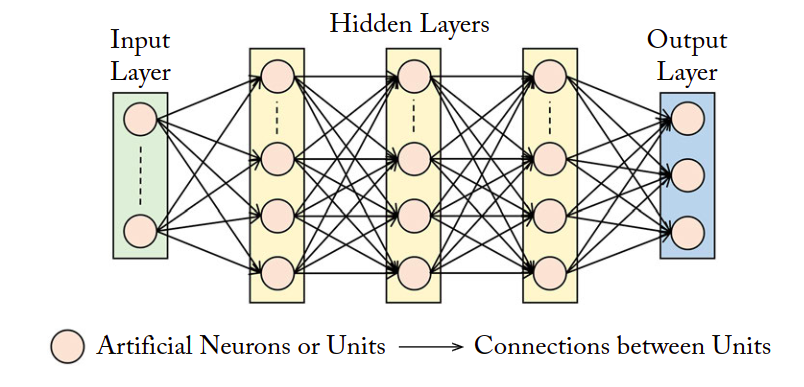
\includegraphics[width=0.6\textwidth]{images/estado_del_arte/multilayer_perceptron.png}
      \caption[Estructura de un perceptrón multicapa (MLP)]{Estructura de un perceptrón multicapa (MLP). Extraído de \cite[fig. 3.1, p.~32]{khan2018guide}.}
   \label{fig:multilayer_perceptron}
\end{figure}

\subsection{Tareas fundamentales en visión por computador} \label{sec:tareas_fundamentales_vision_por_computador}

La visión por computador aborda el desafío de permitir que las máquinas interpreten y comprendan el contenido visual de imágenes y vídeos. Antes del auge del aprendizaje profundo, se empleaban descriptores de características diseñados manualmente, como el \gls{hog}. \gls{hog} captura la forma local de los objetos analizando la distribución de las orientaciones de los gradientes en pequeñas regiones de la imagen (celdas y bloques). La Figura~\ref{fig:hog} muestra una visualización de las características HOG extraídas. Aunque útiles en su momento, estos algoritmos ``hechos a mano'' presentan limitaciones significativas. En particular, no facilitan el aprendizaje por transferencia, es decir, la reutilización de conocimiento aprendido en tareas previas. Además, la complejidad de estas características está intrínsecamente limitada por la capacidad humana para diseñarlas explícitamente. Estos inconvenientes son superados por los algoritmos de aprendizaje automático de características, como las \gls{cnn}, que aprenden representaciones relevantes directamente de los datos. Por ello, las \gls{cnn} han demostrado ser más efectivas en tareas complejas, logrando avances significativos en precisión y eficiencia al aprender automáticamente características a partir de grandes conjuntos de datos.

\begin{figure}[H]
   \centering
   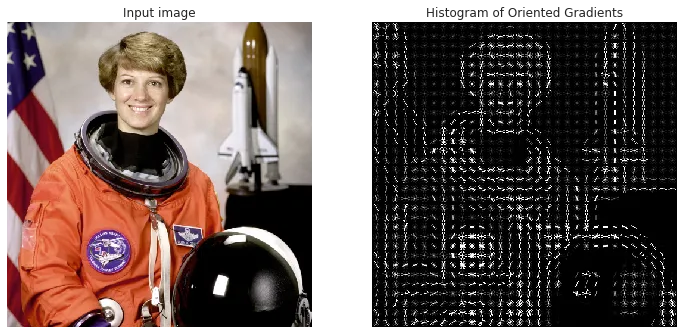
\includegraphics[width=0.6\textwidth]{images/estado_del_arte/HOG_example.png}
   \caption[Ejemplo de HOG aplicado a una imagen]{Ejemplo de HOG aplicado a una imagen. Extraído de \cite{opengenusHOG}.}
   \label{fig:hog}
\end{figure}


En el ámbito del procesamiento de imágenes mediante técnicas de deep learning, existen diversas tareas con diferentes niveles de complejidad:

\begin{enumerate}
    \item \textbf{Clasificación de imágenes}: Es la tarea más básica, donde la red neuronal asigna una etiqueta a toda la imagen. Por ejemplo, determinar si una imagen contiene un perro, gato o coche. El modelo genera un vector de probabilidades para cada clase posible.
    
    \item \textbf{Clasificación con localización}: Además de clasificar el objeto principal, la red también proporciona un cuadro delimitador (bounding box) que indica dónde se encuentra ese objeto en la imagen. Es útil cuando existe un único objeto de interés.
    
   \item \textbf{Detección de objetos}: Extiende la tarea anterior para identificar y localizar múltiples objetos en una imagen. Los algoritmos de detección se dividen principalmente en:
      \begin{itemize}
         \item \textit{Detectores de dos etapas}: Como R-CNN, Fast R-CNN y Faster R-CNN, primero generan propuestas de regiones que podrían contener objetos, y luego clasifican estas regiones. Son más precisos pero computacionalmente más costosos.
         \item \textit{Detectores de una etapa}: Como \gls{yolo} y \gls{ssd} que predicen las cajas delimitadoras y las clases directamente en una sola pasada. Son más rápidos aunque tradicionalmente menos precisos.
      \end{itemize}
      Ambos enfoques proporcionan para cada objeto detectado su clasificación y cuadro delimitador.
    
    \item \textbf{Segmentación}: Es la tarea más compleja, donde la red no solo identifica y localiza objetos, sino que también asigna una etiqueta a cada píxel de la imagen. Esto permite distinguir entre diferentes objetos y sus contornos, facilitando una comprensión más detallada de la escena.
\end{enumerate}

La Figura~\ref{fig:tareas_vision_por_computador} ilustra estas tareas fundamentales en visión por computador. Para este trabajo, nos centraremos en la tarea de detección de objetos, que es esencial para identificar y clasificar varios objetos en movimiento en un vídeo o imagen.

\begin{figure}[H]
   \centering
   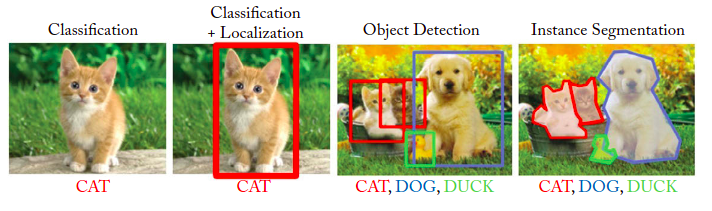
\includegraphics[width=0.8\textwidth]{images/estado_del_arte/diferentes_formas_de_detectar.png}
   \caption[Tareas fundamentales en visión por computador]{Tareas fundamentales en visión por computador. Extraído de \cite[fig. 1.1, p. ~2]{khan2018guide}.}
   \label{fig:tareas_vision_por_computador}
\end{figure}

\subsection{Arquitectura y funcionamiento de las CNN} \label{sec:arquitectura_cnn}
Las \gls{cnn} son un tipo específico de red neuronal profunda. Estas redes están diseñadas para procesar imágenes y extraer características relevantes de manera eficiente, lo que las hace especialmente adecuadas para tareas de visión por computador.

\begin{figure}[H]
   \centering
   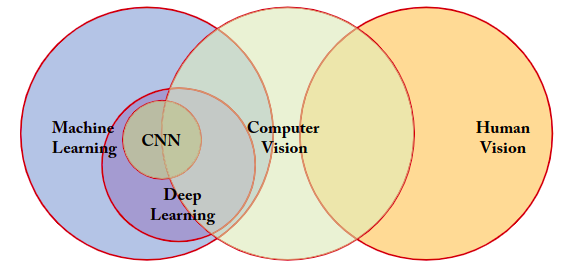
\includegraphics[width=0.6\textwidth]{images/estado_del_arte/diagrama_de_Venn_inteligencia_artificial.png}
   \caption[Relación entre Machine Learning, Deep Learning, CNN, Computer Vision y Human Vision]{Relación entre Machine Learning, Deep Learning, CNN, Computer Vision y Human Vision. Extraído de \cite[fig. 1.3, p. ~7]{khan2018guide}.}
   \label{fig:diagrama_de_Venn_inteligencia_artificial}
\end{figure}

La Figura~\ref{fig:diagrama_de_Venn_inteligencia_artificial} ilustra la relación entre estos conceptos. Las \gls{cnn} son una subcategoría del Deep Learning, que a su vez es una subcategoría del Machine Learning. Además, las \gls{cnn} están estrechamente relacionadas con la visión por computador, que busca emular la capacidad de los humanos para interpretar imágenes y vídeos.

Las \gls{cnn} se inspiran en la forma en que los humanos percibimos el mundo visual. Al igual que nuestro sistema visual, que procesa la información de manera jerárquica, las \gls{cnn} utilizan capas convolucionales para extraer características de bajo nivel (como bordes y texturas) y capas más profundas para identificar patrones y objetos más complejos. Esta jerarquía de características permite a las \gls{cnn} aprender representaciones ricas y abstractas de los datos visuales.

Estas redes se componen de varias capas, cada una de las cuales realiza operaciones específicas en los datos de entrada. Las capas más comunes y técnicas asociadas en una \gls{cnn}, que se describen a continuación, son las capas convolucionales, las capas de activación, las capas de pooling, la normalización por lotes y las capas completamente conectadas.

Las \textbf{capas convolucionales} utilizan la operación de convolución para extraer características. Esta operación es fundamental en las \gls{cnn} y consiste en aplicar un filtro (o kernel) a una imagen para extraer características locales. El filtro se desliza sobre la imagen, multiplicando sus valores por los valores de la imagen en cada posición y sumando los resultados. Este proceso genera un mapa de activación que resalta las características relevantes de la imagen.

\begin{figure}[H]
   \centering
   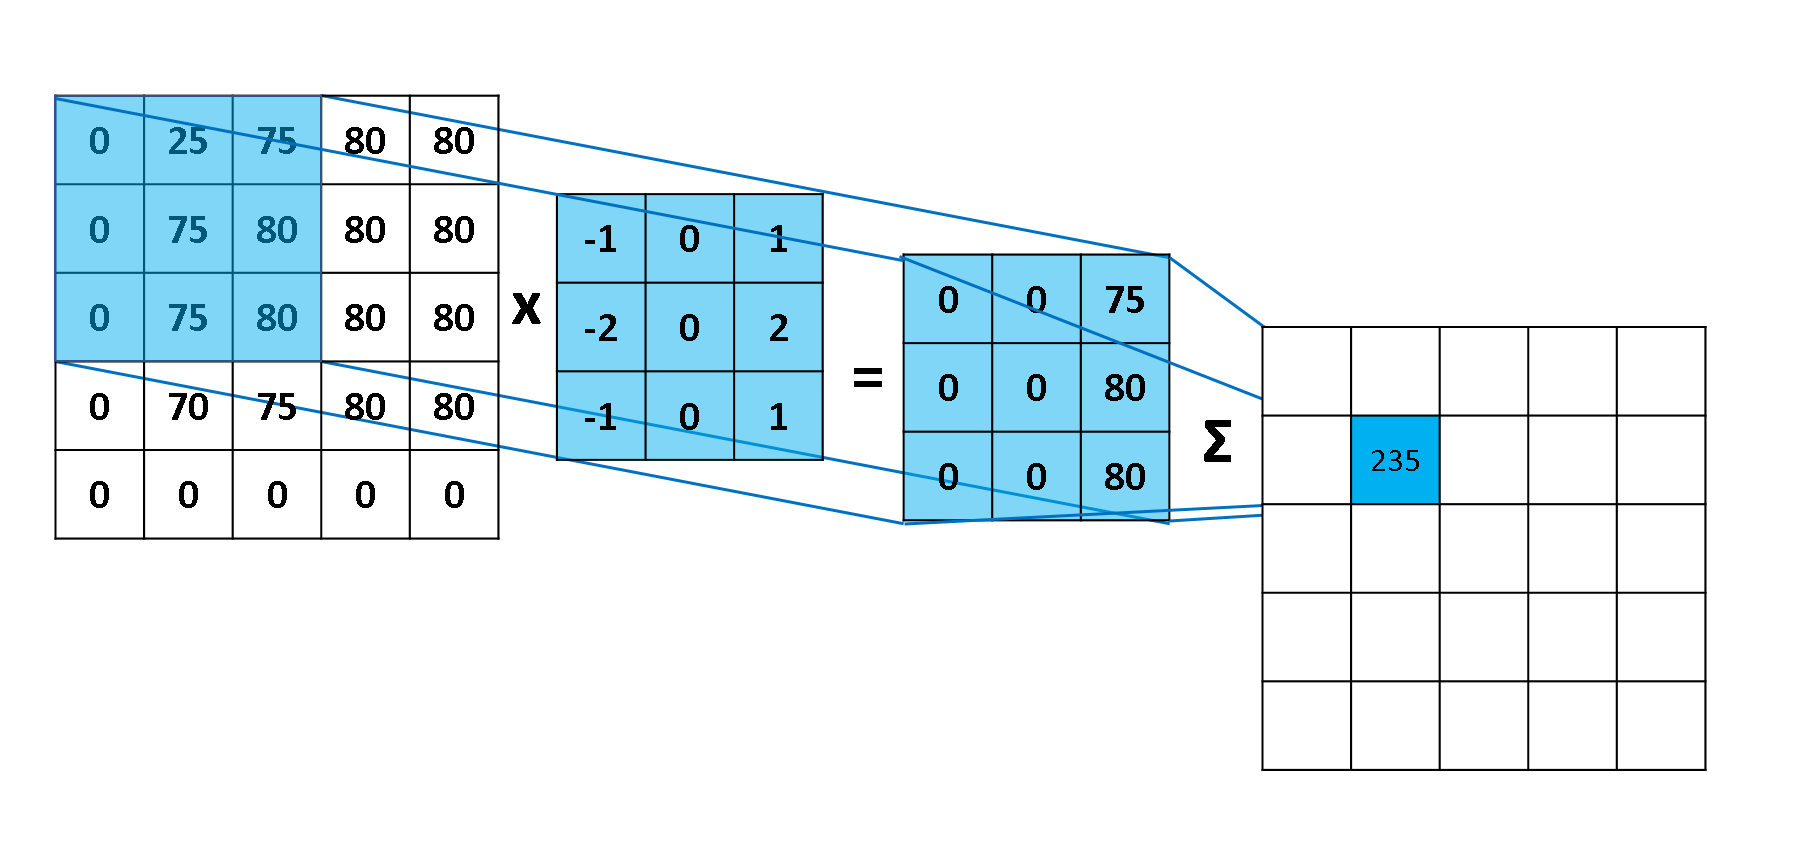
\includegraphics[width=0.7\textwidth]{images/estado_del_arte/operacion_convolucion.png}
   \caption[Operación de convolución sobre los pixeles de una imagen]{Operación de convolución sobre los pixeles de una imagen. Extraído de \cite[fig. 2.5, p. ~48]{khan2018guide}.}
   \label{fig:operacion_convolucion}
\end{figure}

La Figura~\ref{fig:operacion_convolucion} ilustra la operación de una capa de convolución. En este ejemplo, se aplica un filtro de $2 \times 2$ (mostrado en verde) a un mapa de características de entrada de $6 \times 6$ (incluyendo un relleno de ceros de 1) con un paso (stride) de 2. El filtro se desliza sobre la entrada, y en cada paso, se realiza una multiplicación elemento a elemento entre el filtro y la región correspondiente de la entrada. La suma de estos productos genera un valor en el mapa de características de salida (mostrado en azul).

\begin{figure}[H]
   \centering
   \begin{subfigure}[b]{0.25\textwidth}
      \centering
      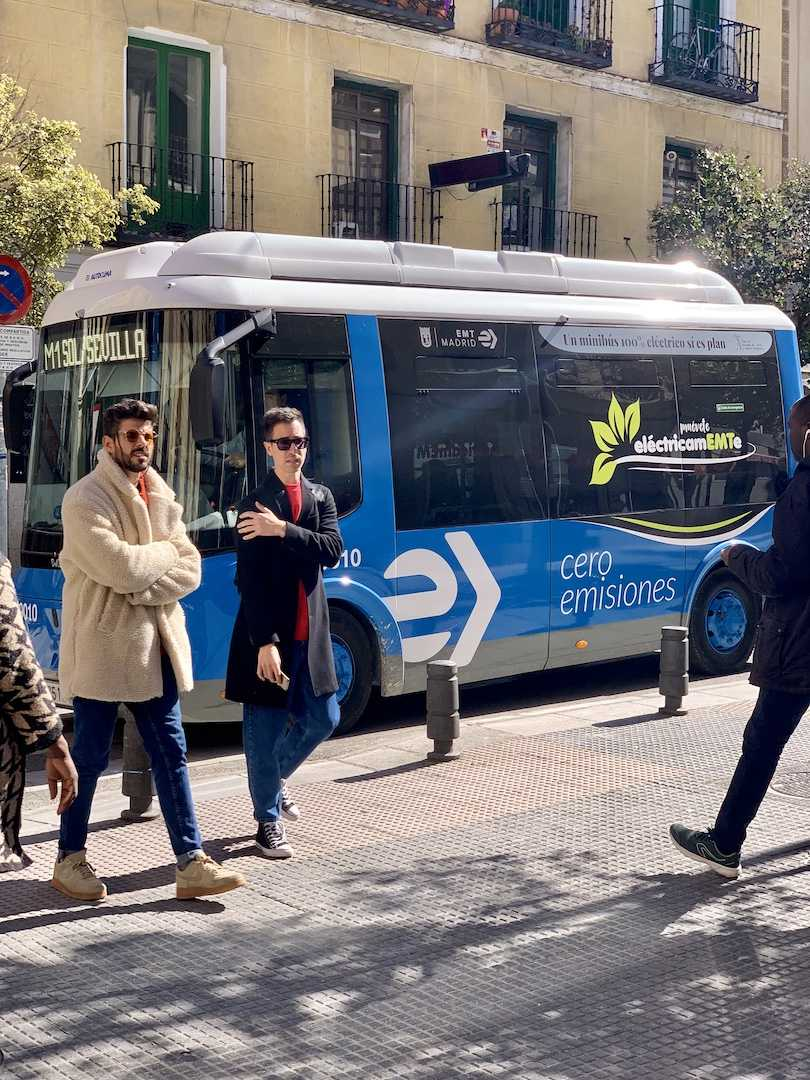
\includegraphics[width=\textwidth]{images/estado_del_arte/bus_original.jpg}
      \caption{Imagen de un autobús.}
      \label{fig:bus_original}
   \end{subfigure}
   \hfill
   \begin{subfigure}[b]{0.7\textwidth}
      \centering
      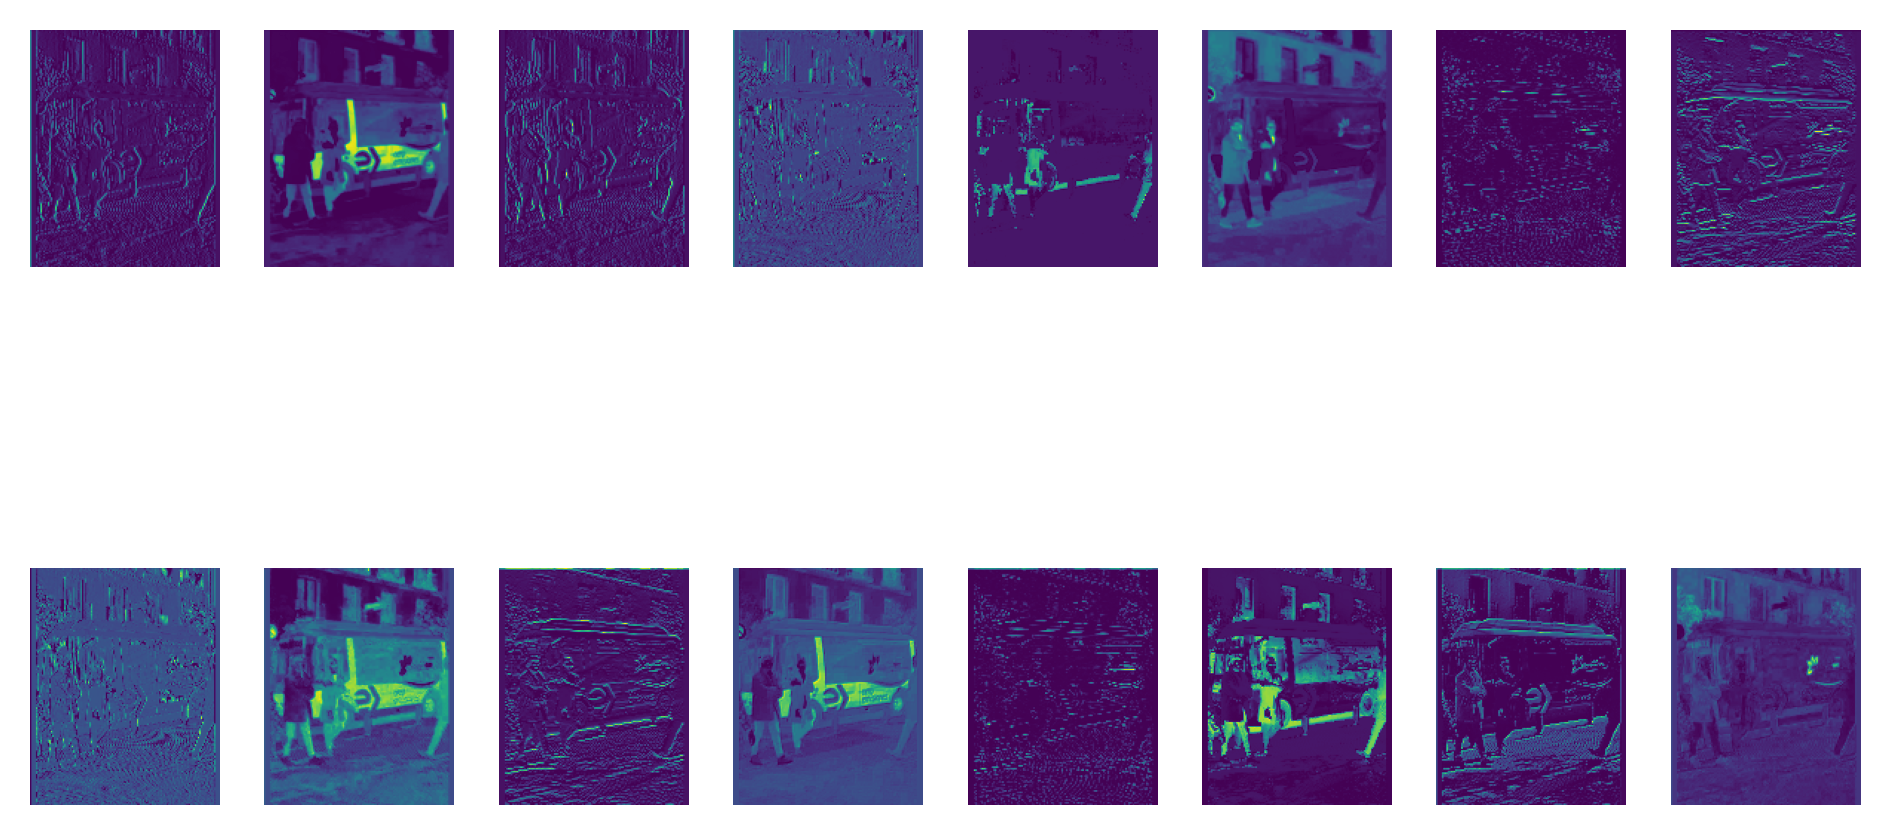
\includegraphics[width=\textwidth]{images/estado_del_arte/bus_primera_capa_convolucion.png}
      \caption{Resultado de la operación de convolución.}
      \label{fig:bus_primera_capa_convolucion}
   \end{subfigure}
   \caption{Proceso de convolución aplicado a una imagen de un autobús.}
   \label{fig:bus_convolucion}
\end{figure}

La Figura~\ref{fig:bus_convolucion} ilustra el proceso de la primera convolución del modelo YOLO11n \cite{yolo11_ultralytics}. En la parte izquierda se muestra la imagen original de un autobús, mientras que en la parte derecha se presenta el resultado de aplicar la operación de convolución. En este caso, los 16 filtros de la primera capa convolucional han detectado diferentes características de la imagen, como bordes y texturas. Este proceso se repite en múltiples capas, lo que permite a la red aprender representaciones cada vez más complejas de la imagen.

Las \textbf{capas de activación}, especialmente la ReLU (Rectified Linear Unit), son fundamentales para introducir no-linealidad en el modelo. La función ReLU transforma cada valor negativo en cero mientras mantiene los valores positivos sin cambios, lo que ayuda a mitigar el problema del desvanecimiento del gradiente y acelera el proceso de entrenamiento. La función ReLU se define como:
\begin{equation}
   f(x) = \begin{cases}
      0 & \text{si } x < 0 \\
      x & \text{si } x \geq 0
   \end{cases}
\end{equation}
Estas capas se aplican típicamente después de cada capa convolucional y completamente conectada.

Las \gls{cnn} incorporan \textbf{capas de pooling} (o submuestreo). Estas capas desempeñan un papel crucial en la reducción progresiva de la dimensión espacial (ancho y alto) de los mapas de características, lo que conlleva varios beneficios importantes: disminuyen la cantidad de parámetros y la carga computacional, ayudan a controlar el sobreajuste (\textit{overfitting}) al reducir la complejidad del modelo, y proporcionan un cierto grado de invarianza a pequeñas traslaciones y distorsiones. El funcionamiento del pooling implica deslizar una ventana sobre el mapa de características de entrada y aplicar una operación de agregación. Las operaciones más comunes son Max-Pooling, que selecciona el valor máximo dentro de la ventana (eficaz para capturar las características más prominentes, como se ilustra en la Figura~\ref{fig:pooling}), y Average-Pooling, que calcula el valor promedio (tiende a suavizar las características). El resultado es un mapa de características de menor tamaño pero que conserva la información esencial.

\begin{figure}[H]
   \centering
   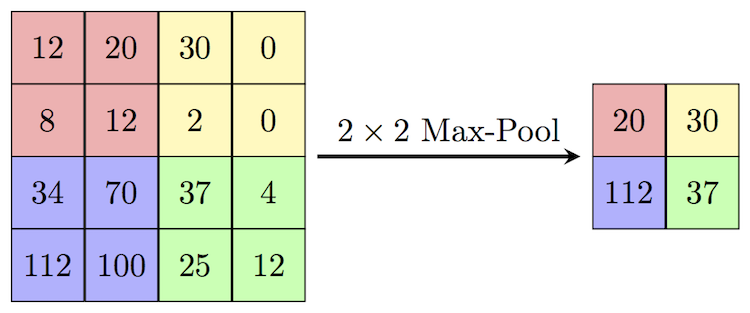
\includegraphics[width=0.6\textwidth]{images/estado_del_arte/max_pooling.png}
   \caption[Ejemplo de operación de max-pooling con una ventana de $2 \times 2$ y un \textit{stride} de 2]{Ejemplo de operación de max-pooling con una ventana de $2 \times 2$ y un \textit{stride} de 2. Se selecciona el valor máximo de cada región de color. Extraído de \cite{csWikiMaxpoolSample}.}
   \label{fig:pooling}
\end{figure}

La \textbf{Normalización por Lotes} (\textit{Batch Normalization}, BN) es una técnica fundamental para mitigar el problema del \textit{cambio interno de covariables} (\textit{internal covariate shift}), que es la alteración de la distribución de las activaciones intermedias durante el entrenamiento. BN opera a nivel de mini-lotes $\mathcal{B} = \{x_1, \dots, x_m\}$, calculando la media $\mu_{\mathcal{B}}$ y la varianza $\sigma^2_{\mathcal{B}}$:
\begin{align}
   \mu_{\mathcal{B}} &= \frac{1}{m} \sum_{i=1}^{m} x_i \\
   \sigma^2_{\mathcal{B}} &= \frac{1}{m} \sum_{i=1}^{m} (x_i - \mu_{\mathcal{B}})^2
\end{align}
Luego, normaliza cada activación $x_i$:
\begin{equation}
   \hat{x}_i = \frac{x_i - \mu_{\mathcal{B}}}{\sqrt{\sigma^2_{\mathcal{B}} + \epsilon}}
\end{equation}
donde $\epsilon$ es una constante pequeña para estabilidad numérica. Para preservar la capacidad expresiva, BN introduce parámetros aprendibles $\gamma$ (escala) y $\beta$ (desplazamiento) para realizar una transformación afín:
\begin{equation}
   y_i = \gamma \hat{x}_i + \beta
\end{equation}
La salida $y_i$ se propaga a la siguiente operación. BN estabiliza y acelera el entrenamiento, permite tasas de aprendizaje más altas y tiene un efecto regularizador que ayuda a prevenir el sobreajuste. Se inserta típicamente después de capas convolucionales o totalmente conectadas, antes de la activación.

En el final de la red, se utilizan \textbf{capas completamente conectadas} (\textit{fully connected}). Estas capas toman las características de alto nivel extraídas por las capas anteriores y las combinan para realizar la tarea final, como la clasificación de objetos. Cada neurona en una capa completamente conectada está conectada a todas las neuronas de la capa anterior. En la salida final, se utiliza una función de activación como Softmax para convertir las salidas en probabilidades de clase. La función Softmax se define como:

\begin{equation}
   \sigma(z_i) = \frac{e^{z_i}}{\sum_{j=1}^{K} e^{z_j}}
\end{equation}
donde $z = (z_1, \dots, z_K)$ es el vector de salidas de la capa anterior para $K$ clases. La función Softmax transforma este vector en un vector de probabilidades $\sigma(z) = (\sigma(z_1), \dots, \sigma(z_K))$, donde cada componente $\sigma(z_i)$ se calcula como se muestra. El resultado es un vector de tamaño $K$ donde cada elemento está en el rango (0, 1) y la suma de todos los elementos es igual a 1 ($\sum_{j=1}^{K} \sigma(z_j) = 1$). Esto permite interpretar la salida como una distribución de probabilidad sobre las $K$ posibles clases.

En la Figura~\ref{fig:cnn_example} se muestra un ejemplo de una \gls{cnn} simple. Esta red incluye capas convolucionales para la extracción de características, capas de activación para introducir no linealidad, capas de pooling para reducir la dimensionalidad y capas completamente conectadas para realizar la clasificación final. La combinación de estas capas permite a las \gls{cnn} aprender representaciones jerárquicas y complejas de los datos visuales, lo que las convierte en una herramienta poderosa para tareas de visión por computador.

\begin{figure}[H]
   \centering
   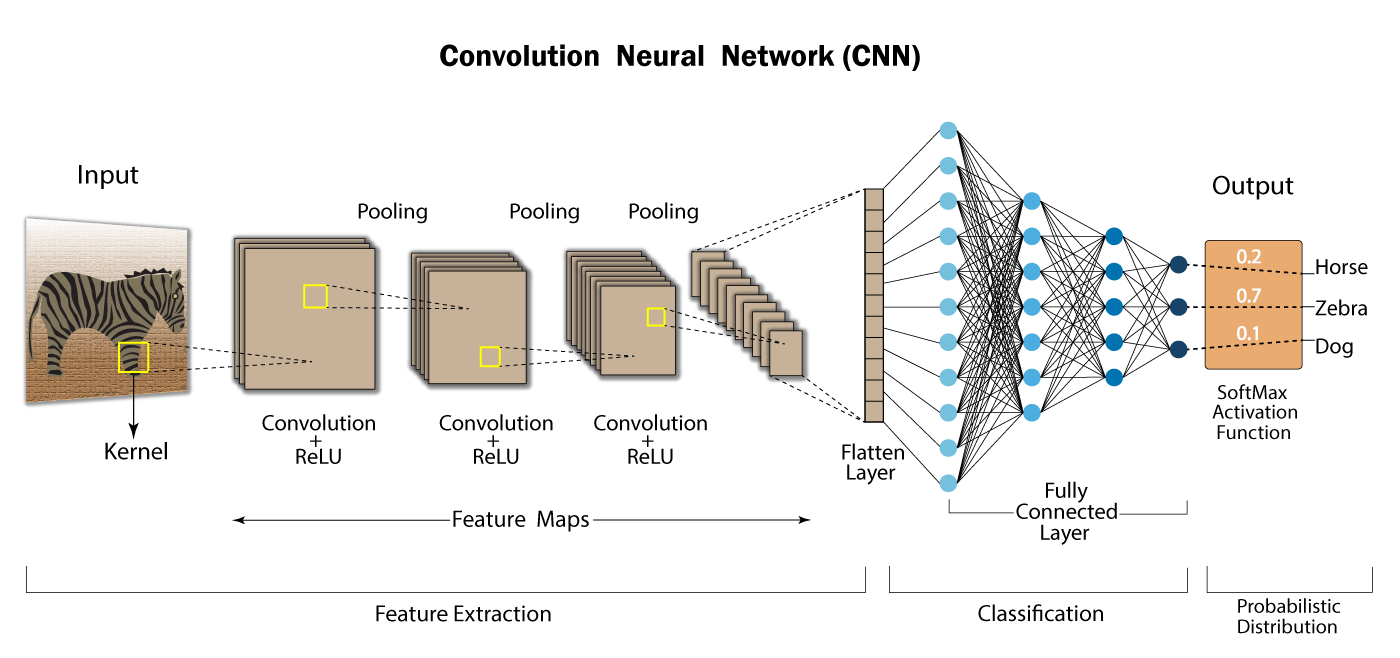
\includegraphics[width=0.9\textwidth]{images/estado_del_arte/cnn_example.png}
   \caption[Ejemplo de una CNN simple]{Ejemplo de una CNN simple. Extraído de \cite{devbreachCNN}.}
   \label{fig:cnn_example}
\end{figure}


Tras comprender la arquitectura interna de las \gls{cnn}, el siguiente paso es el entrenamiento. Este proceso se basa fundamentalmente en el uso de un conjunto de datos etiquetado, que actúa como la verdad fundamental (\textit{ground truth}). Este conjunto contiene una colección de imágenes junto con sus correspondientes etiquetas o anotaciones, que la red utilizará para aprender.

El objetivo principal del entrenamiento es ajustar los parámetros internos de la \gls{cnn} (pesos y sesgos) para minimizar una función de pérdida predefinida. Esta función mide la discrepancia o el error entre las predicciones generadas por la red y las etiquetas reales proporcionadas en los datos de entrenamiento.

El proceso de ajuste se realiza de forma iterativa mediante un algoritmo de optimización. El Descenso de Gradiente Estocástico (SGD) y sus variantes, como Adam o RMSprop, son opciones comunes. Estos algoritmos utilizan el cálculo de gradientes para determinar cómo modificar los pesos y sesgos para reducir el error.

El mecanismo central de este ajuste implica dos fases: la propagación hacia adelante (\textit{forward propagation}) y la retropropagación (\textit{backpropagation}). Durante la propagación hacia adelante, los datos de entrada atraviesan las capas de la red para generar una salida. Esta salida se compara con la etiqueta real mediante la función de pérdida. En la retropropagación, el algoritmo calcula el gradiente del error con respecto a los pesos y sesgos, utilizando la regla de la cadena. Estos gradientes guían la actualización de los parámetros.

Típicamente, todo el conjunto de datos de entrenamiento se procesa varias veces en ciclos conocidos como épocas. Este refinamiento iterativo continúa hasta que el rendimiento de la red, evaluado en un conjunto de datos de validación separado (que no se utiliza para el entrenamiento directo), alcanza un nivel satisfactorio. La validación es crucial para asegurar que el modelo generaliza bien a datos no vistos previamente.

Además, para prevenir el sobreajuste (\textit{overfitting}) —donde el modelo aprende demasiado bien los datos de entrenamiento pero falla en generalizar— se emplean técnicas de regularización. El \textit{dropout} es una técnica común que desactiva aleatoriamente un porcentaje de neuronas durante cada iteración de entrenamiento, forzando a la red a aprender representaciones más robustas. La normalización por lotes (\textit{batch normalization}), explicada previamente, también actúa como regularizador y ayuda a estabilizar el entrenamiento.

En escenarios prácticos, desarrollar y entrenar una \gls{cnn} desde cero puede ser computacionalmente costoso y requerir grandes cantidades de datos etiquetados.

Por lo tanto, una estrategia común y muy eficaz consiste en aprovechar modelos preentrenados. Arquitecturas como VGG16, ResNet50 y MobileNetV2, que han sido entrenadas previamente en conjuntos de datos de referencia masivos como ImageNet (que contiene millones de imágenes en miles de categorías) o COCO (centrado en la detección y segmentación de objetos), sirven como puntos de partida potentes. Estos modelos ya han aprendido características jerárquicas ricas a partir de datos visuales diversos.

Mediante una técnica conocida como \textit{transfer learning} o aprendizaje por transferencia, estos modelos preentrenados pueden adaptarse eficientemente a tareas nuevas y específicas, incluso con conjuntos de datos personalizados más pequeños. El aprendizaje por transferencia generalmente implica tomar las capas de extracción de características del modelo preentrenado (la base convolucional) y ajustarlas (\textit{fine-tuning}) o añadir nuevas capas de clasificación adaptadas a la tarea objetivo.

Este enfoque acelera significativamente el proceso de entrenamiento para la nueva tarea y, a menudo, conduce a un mejor rendimiento en comparación con el entrenamiento desde cero, ya que transfiere eficazmente el conocimiento visual general adquirido durante el entrenamiento inicial a gran escala.





\subsection{Detectores de dos etapas} \label{sec:two_stage_detectors}
Los detectores de dos etapas, funcionan mediante un proceso secuencial: primero generan propuestas de regiones (region proposals) que podrían contener objetos y posteriormente clasifican estas regiones. Este enfoque favorece la precisión, aunque generalmente a costa de un mayor tiempo de procesamiento.

La primera arquitectura exitosa de detección de objetos basada en deep learning fue R-CNN (Regions with CNN features) \cite{girshick2014richfeaturehierarchiesaccurate}. Este modelo introdujo un enfoque de dos etapas que revolucionó el campo. En su primera fase, R-CNN utiliza un algoritmo de búsqueda selectiva (Selective Search) para generar aproximadamente 2,000 propuestas de regiones que podrían contener objetos. Este algoritmo de búsqueda selectiva divide la imágen en nodos y aristas, e iterativamente agrupa estas regiones en función del color, textura, tamaño y forma hasta que se obtienen las propuestas finales. En la figura \ref{fig:selective_search} se muestra un ejemplo del resultado del algoritmo de búsqueda selectiva.

\begin{figure}[H]
   \centering
   \begin{subfigure}[b]{0.45\textwidth}
      \centering
      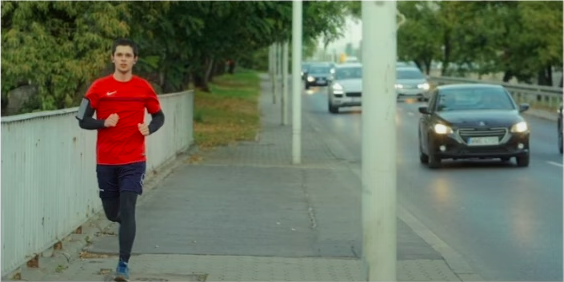
\includegraphics[width=\textwidth]{images/estado_del_arte/selective_search_original.png}
      \caption{Imagen original.}
      \label{fig:selective_search_original}
   \end{subfigure}
   \hfill
   \begin{subfigure}[b]{0.45\textwidth}
      \centering
      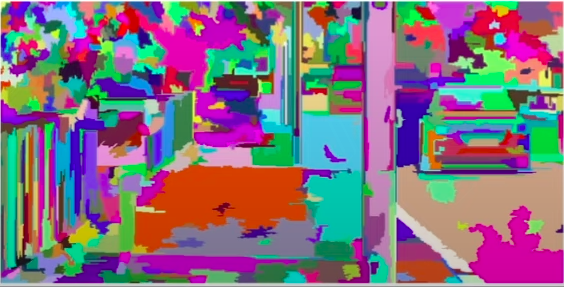
\includegraphics[width=\textwidth]{images/estado_del_arte/selective_search_result.png}
      \caption{Resultado de búsqueda selectiva.}     
      \label{fig:selective_search_result}
   \end{subfigure}
   \caption[Proceso de búsqueda selectiva aplicado a una imagen]{Proceso de búsqueda selectiva aplicado a una imagen. Extraído de \cite{explainningAI}.}
   \label{fig:selective_search}
\end{figure}

En la segunda fase, cada región propuesta es redimensionada y procesada individualmente por una \gls{cnn} para extraer características de alto nivel. Estas características alimentan posteriormente a un clasificador SVM (Support Vector Machine) para determinar la categoría del objeto y a un regresor lineal para mejorar la localización del cuadro delimitador. Como se ilustra en la Figura~\ref{fig:r-cnn}, este enfoque fue innovador pero computacionalmente costoso, ya que requiere procesar cada propuesta de región de manera independiente.

\begin{figure}[H]
   \centering
   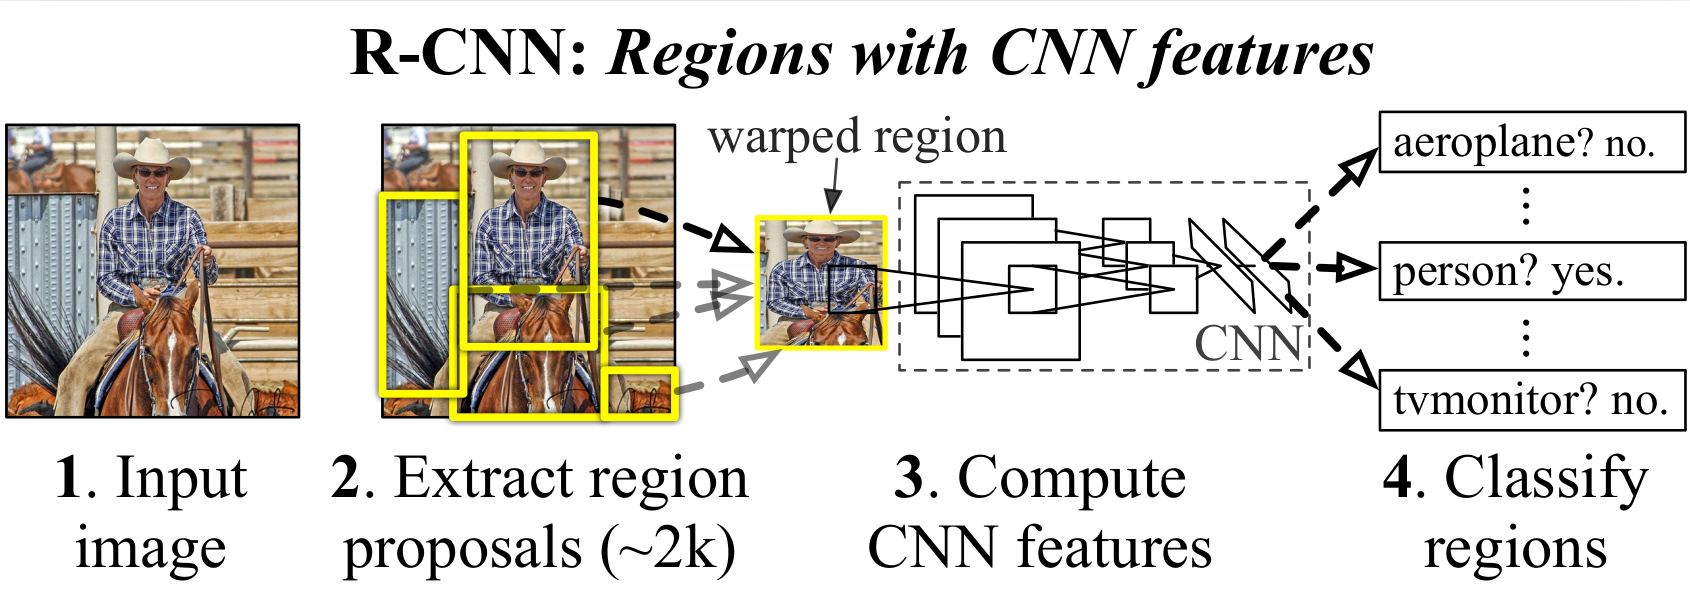
\includegraphics[width=0.6\textwidth]{images/estado_del_arte/R-CNN.png}
   \caption[Arquitectura de R-CNN]{Arquitectura de R-CNN. Extraído de \cite[fig. 1, p. ~1]{girshick2014richfeaturehierarchiesaccurate}.}
   \label{fig:r-cnn}
\end{figure}

\subsection{Detectores de una etapa}\label{sec:one_stage_detectors}
%https://www.ultralytics.com/es/glossary/one-stage-object-detectors Explicación de los detectores de 1 etapa por Ultralytics
%https://www.ultralytics.com/glossary/backbone Explicación de la parte de backbone en los detectores de 1 etapa por Ultralytics
%https://www.ultralytics.com/glossary/anchor-free-detectors Explicación de los detectores anchor-free por Ultralytics
%https://sharkyun.medium.com/computer-vision-object-detection-one-stage-vs-two-stage-b05dbff88195 Explicación simple de las diferencias entre los detectores de 2 etapas frente a los de 1 etapa

En contraste con los detectores de dos etapas, los detectores de una etapa (one-stage detectors) adoptan un enfoque más directo y eficiente. Estos detectores realizan la localización y clasificación de objetos simultáneamente en una sola pasada a través de la red, sin necesidad de un paso intermedio de generación de propuestas.

La arquitectura de los detectores de una etapa procesa la imagen completa una única vez, típicamente mediante una red troncal o \textit{backbone} (generalmente una \gls{cnn}) para la extracción de características. Estas características son posteriormente procesadas por componentes intermedios (\textit{neck}) y alimentadas a una cabeza de detección (\textit{detection head}) que predice simultáneamente las coordenadas de los cuadros delimitadores (\textit{bounding boxes}) y las probabilidades de clase.
Esta arquitectura de una etapa prioriza la velocidad de inferencia, resultando idónea para aplicaciones en tiempo real donde la latencia es un factor crítico, aunque pueda suponer una ligera concesión en la precisión máxima. Modelos representativos de este enfoque incluyen \gls{ssd} (Single Shot MultiBox Detector)\cite{Liu_2016} y \gls{yolo} (You Only Look Once)\cite{redmon2016lookonceunifiedrealtime}. Estos han demostrado un equilibrio eficaz entre rapidez y exactitud, permitiendo la detección en tiempo real incluso en dispositivos con recursos computacionales limitados.

\gls{yolo} se destaca como una de las arquitecturas de detección de objetos más populares y efectivas. Concebida específicamente para la detección en tiempo real, \gls{yolo} introdujo un enfoque unificado que procesa la imagen completa en una sola pasada, realizando la localización y clasificación de forma simultánea. Esta metodología ha sido fundamental para su adopción en aplicaciones que requieren alta velocidad de procesamiento.

\gls{yolo} en su primera versión procesa la imagen completa de una vez. Divide la imagen en una cuadrícula de $S \times S$ celdas. Cada celda es responsable de detectar los objetos cuyo centro se encuentre dentro de ella. Para cada celda, \gls{yolo} predice $B$ cuadros delimitadores (bounding boxes) y puntuaciones de confianza para esos cuadros. La puntuación de confianza indica la probabilidad de que haya un objeto en el cuadro y la precisión de la predicción del cuadro. Al mismo tiempo, predice las probabilidades de clase para cada objeto detectado en la celda.

\begin{figure}[H]
   \centering
   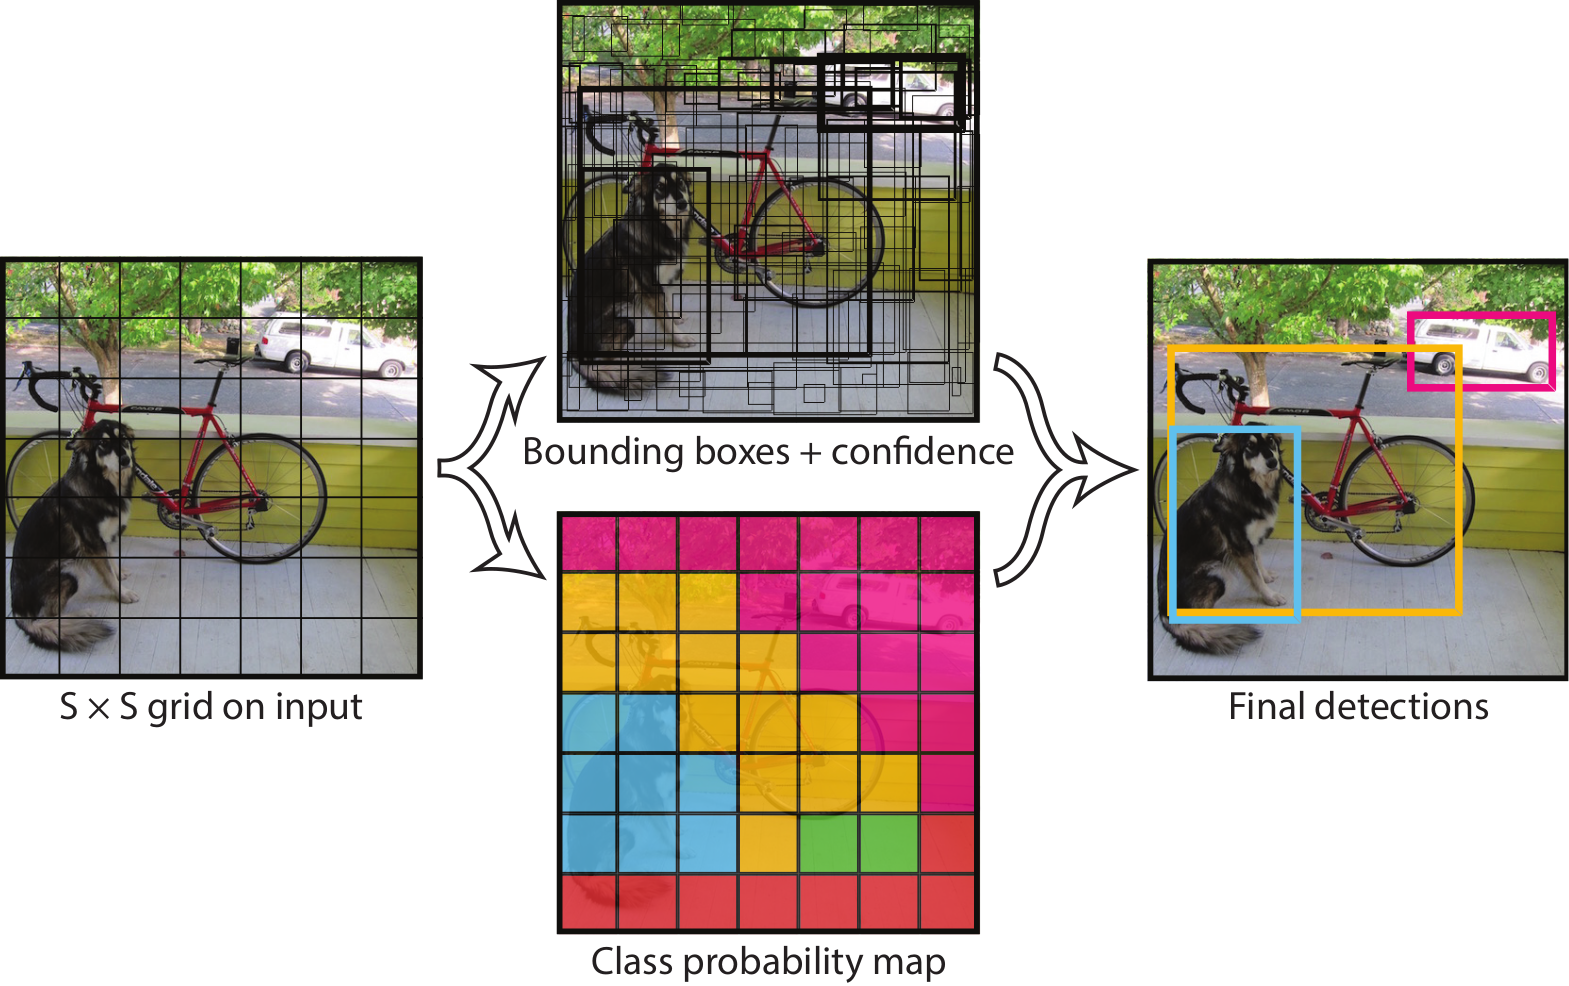
\includegraphics[width=0.8\textwidth]{images/estado_del_arte/yolo_detections_example.png}
   \caption[Ejemplo de detección de objetos utilizando YOLO]{Ejemplo de detección de objetos utilizando YOLO. Extraído de \cite[fig. 2, p. ~2]{redmon2016lookonceunifiedrealtime}.}
   \label{fig:yolo_detections_example}
\end{figure}

Como se ilustra en la Figura~\ref{fig:yolo_detections_example}, \gls{yolo} modela la detección como un problema de regresión. Las predicciones del modelo se codifican como una matriz de 3 dimensiones de  $S \times S \times (B * 5 + C)$, donde el factor $5$ corresponde a las coordenadas $x$, $y$, ancho, alto y la puntuación de confianza para cada cuadro delimitador, mientras que $C$ representa el número de clases posibles. Por ejemplo, si se utilizan $B=2$ cuadros delimitadores (por cada celda, es decir, cada celda realiza 2 predicciones) y $C=20$ clases, el tensor de salida tendrá dimensiones $S \times S \times (2 * 5 + 20)$. 

Una vez generadas las predicciones, \gls{yolo} implementa un post-procesamiento mediante \gls{nms} para eliminar detecciones redundantes y conservar únicamente las más precisas. El algoritmo \gls{nms} funciona de la siguiente manera:

\begin{enumerate}
   \item \textbf{Ordenamiento por Confianza:} Las cajas delimitadoras detectadas se ordenan por su puntuación de confianza, de mayor a menor.
   \item \textbf{Selección de la Detección Más Confiable:} Se selecciona la caja delimitadora con la puntuación de confianza más alta y se añade a la lista de detecciones finales.
   \item \textbf{Cálculo de la Intersección sobre Unión (IoU):} Se calcula la \gls{iou} entre la caja delimitadora seleccionada y todas las demás cajas delimitadoras restantes.
   \item \textbf{Eliminación de Detecciones Redundantes:} Se eliminan todas las cajas delimitadoras con una \gls{iou} superior a un umbral predefinido con la caja delimitadora seleccionada.
   \item \textbf{Iteración:} Se repiten los pasos 2-4 hasta que no queden más cajas delimitadoras por procesar.
\end{enumerate}

En resumen, \gls{nms} evalúa la superposición entre las cajas y elimina aquellas que exceden un cierto umbral con la caja de mayor confianza, asegurando que solo las detecciones más precisas y no redundantes se conserven, mejorando la calidad general de las detecciones.

Este enfoque unificado permite que \gls{yolo} procese imágenes a velocidades significativamente mayores que los detectores de dos etapas, mientras mantiene una precisión competitiva, lo que lo hace ideal para aplicaciones en tiempo real como las que se abordan en este trabajo.

\begin{figure}[H]
   \centering
   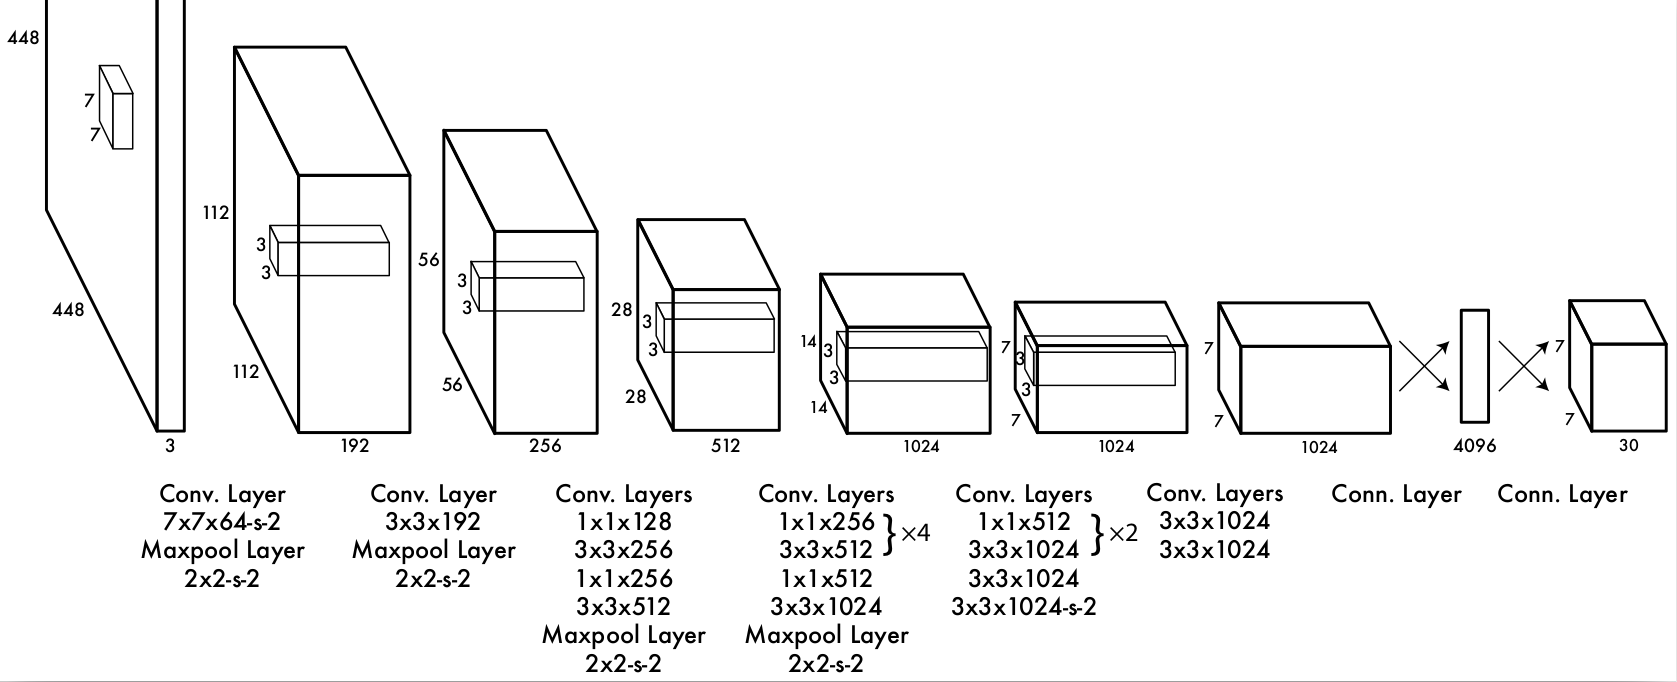
\includegraphics[width=0.8\textwidth]{images/estado_del_arte/yolo_architecture.png}
   \caption[Arquitectura de YOLO]{Arquitectura de YOLO. Extraído de \cite[fig. 3, p. ~3]{redmon2016lookonceunifiedrealtime}.}
   \label{fig:yolo_architecture}
\end{figure}

En la Figura~\ref{fig:yolo_architecture} se presenta la arquitectura del modelo primigenio de \gls{yolo} \cite{redmon2016lookonceunifiedrealtime}. Esta arquitectura se basa en una red neuronal convolucional que extrae características de la imagen de entrada y las procesa a través de varias capas para generar las predicciones finales. A lo largo de los años, se han desarrollado múltiples versiones y mejoras de \gls{yolo}, cada una optimizando aspectos como la precisión, la velocidad y la capacidad de detección de objetos pequeños o densamente agrupados.

En este proyecto, se han seleccionado diversas versiones de YOLOV5 \cite{yolov5_ultralytics}, YOLOV8 \cite{yolov8_ultralytics} y YOLO11 \cite{yolo11_ultralytics}. Estas representan mejoras y optimizaciones sobre arquitecturas \gls{yolo} anteriores. Los modelos mencionados forman parte de la librería Ultralytics \cite{Jocher_Ultralytics_YOLO_2023}, que proporciona una implementación eficaz y sencilla de varias variantes de \gls{yolo}. Las aportaciones de Ultralytics a la comunidad de visión artificial son notables, ya que sus herramientas y recursos facilitan el ciclo de vida completo (entrenamiento, evaluación, implementación) de los modelos \gls{yolo}.

\subsection{Métricas de evaluación de modelos de detección de objetos} \label{sec:metricas_evaluacion}

Para evaluar el rendimiento de los modelos de detección de objetos, se utilizan métricas específicas que permiten cuantificar la precisión y efectividad del sistema. Entre las métricas más comunes se encuentran:

\begin{itemize}
   \item \textbf{Precisión}: Mide la proporción de verdaderos positivos (TP) respecto al total de predicciones positivas realizadas por el modelo. Se calcula como:
   \[
   \text{Precision} = \frac{TP}{TP + FP}
   \]
   donde $FP$ representa los falsos positivos. Una alta precisión indica que el modelo realiza pocas predicciones incorrectas.

   \item \textbf{Recall}: Mide la proporción de verdaderos positivos respecto al total de objetos relevantes en la imagen. Se calcula como:
   \[
   \text{Recall} = \frac{TP}{TP + FN}
   \]
   donde $FN$ representa los falsos negativos. Un alto recall indica que el modelo es capaz de detectar la mayoría de los objetos relevantes, aunque pueda incluir algunas predicciones incorrectas.

   \item \textbf{IoU (Intersection over Union)}: Mide la superposición entre el cuadro delimitador predicho y el cuadro delimitador real. Se calcula como:
   \[
   \text{IoU} = \frac{\text{Area de interseccion}}{\text{Area de union}}
   \]

   Una IoU alta indica que el modelo ha localizado correctamente el objeto. Generalmente, se considera que una IoU superior a 0.5 indica una detección correcta.

   \item \textbf{mAP (mean Average Precision)}: Es una métrica que combina precisión y recall, promediando la precisión a diferentes niveles de recall. Se utiliza para evaluar el rendimiento general del modelo en múltiples clases. 
   
   El cálculo del mAP se realiza en varios pasos: primero, para cada clase se calcula la curva PR (Precision-Recall) y se obtiene el Average Precision (AP), que representa el área bajo esta curva. Luego, el mAP se obtiene como la media de todos los AP de las diferentes clases. En detección de objetos, el mAP suele incorporar diferentes umbrales de IoU (Intersection over Union), expresándose como mAP@IoU=0.5 o mAP@IoU=0.5:0.95. Esta métrica es especialmente útil cuando las clases están desequilibradas, ya que da igual importancia a clases minoritarias y mayoritarias. Un valor de mAP cercano a 1 indica un modelo con alta precisión y recall en todas las clases.

   \item \textbf{Latencia}: Mide el tiempo que tarda el modelo en procesar una imagen y generar una predicción se mide en milisegundos (ms) y un valor bajo indica que el modelo es capaz de realizar inferencias rápidamente.
   
   \item \textbf{FPS (Frames Per Second)}: Mide la velocidad de procesamiento del modelo, indicando cuántas imágenes puede procesar por segundo; un alto valor de FPS indica que el modelo es capaz de realizar inferencias rápidamente.
   \item \textbf{F1 Score}: Es la media armónica entre precisión y recall, proporcionando un balance entre ambos. Se utiliza para evaluar el rendimiento del modelo en situaciones donde hay un desbalance entre clases. Se calcula como:
   \[
   \text{F1 Score} = 2 \cdot \frac{\text{Precision} \cdot \text{Recall}}{\text{Precision} + \text{Recall}}
   \]

   Un F1 Score alto indica que el modelo tiene un buen equilibrio entre precisión y recall, lo que es especialmente importante en aplicaciones donde tanto la detección correcta como la minimización de falsos positivos son críticas.

   \item \textbf{Loss (Pérdida)}: Es una medida de la discrepancia entre las predicciones del modelo y las etiquetas reales. Durante el entrenamiento, el objetivo es minimizar esta pérdida. Existen diferentes tipos de funciones de pérdida, como la pérdida de clasificación (Cross-Entropy Loss) y la pérdida de localización (Smooth L1 Loss), que se combinan para evaluar el rendimiento del modelo.

\end{itemize}


\section{Aceleradores de procesamiento gráfico} \label{sec:hardware}
Un aspecto fundamental para el despliegue eficiente de modelos de inteligencia artificial es el hardware utilizado para su ejecución. A continuación, se analizan los principales aspectos de los aceleradores de procesamiento gráfico y su importancia en aplicaciones de visión artificial.

\subsection{Limitaciones del hardware tradicional} \label{sec:limitaciones_hardware}

La Dennard Scaling\cite{dennard1974design}, formulada por Robert Dennard en 1974, establecía que a medida que los transistores se reducían de tamaño, su consumo de energía por unidad de área se mantenía constante. Esto significaba que, al reducir el tamaño de los transistores a la mitad, su área se reducía a un cuarto, pero su consumo de energía por unidad de área permanecía igual. Como resultado, el consumo total de energía se reducía a la mitad, permitiendo aumentar la frecuencia de reloj y el número de transistores sin incrementar significativamente el consumo total de energía. Este principio fue fundamental para el avance exponencial en el rendimiento de los procesadores durante décadas. Sin embargo, a partir de 2005, la Dennard Scaling dejó de cumplirse debido a varios factores físicos fundamentales. A escalas nanométricas, los efectos cuánticos y las fugas de corriente se volvieron significativos, impidiendo que el consumo de energía por unidad de área se mantuviera constante.

Por otro lado, la ley de Moore\cite{moore1965cramming}, formulada por Gordon Moore en 1965, predecía que el número de transistores en un chip se duplicaría aproximadamente cada año, predicción que posteriormente se ajustó a cada dos años. Durante décadas, esta ley se cumplió con notable precisión, permitiendo un crecimiento exponencial en la capacidad de procesamiento. Sin embargo, a medida que los transistores se acercan a escalas atómicas (actualmente en torno a los 3-5 nanómetros), los límites físicos y los desafíos de fabricación han ralentizado significativamente este ritmo de avance. Los costes de investigación y desarrollo para mantener esta tendencia se han disparado, y los beneficios en términos de rendimiento por transistor se han reducido.

\begin{figure}[H]
   \centering
   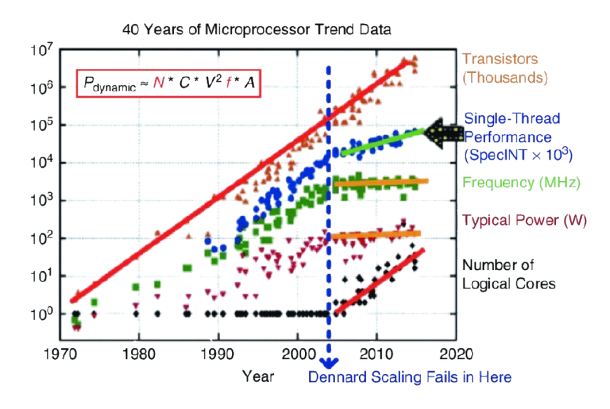
\includegraphics[width=0.8\textwidth]{images/estado_del_arte/dennard_scaling.png}
   \caption[Evolución histórica de las características de los microprocesadores (1970--2020)]{Evolución histórica de las características de los microprocesadores (1970--2020). Extraído de~\cite[p.~8]{ConteRebootingComputing}.}
   \label{fig:dennard_scaling}
\end{figure}

En la Figura~\ref{fig:dennard_scaling} se ilustra claramente el impacto combinado del fin de la Dennard Scaling y el estancamiento de la ley de Moore. La gráfica muestra cinco métricas fundamentales en escala logarítmica: el número de transistores (triángulos naranja) que sigue la ley de Moore, el rendimiento de un solo hilo (círculos azules), la frecuencia de reloj (cuadrados verdes), el consumo de potencia (triángulos invertidos morados) y el número de núcleos lógicos (rombos negros). La ecuación de potencia dinámica ($P_{dynamic} \approx N * C * V^2 * f * A$) explica la relación entre el número de transistores ($N$), la capacitancia ($C$), el voltaje ($V$), la frecuencia ($f$) y el factor de actividad ($A$).

El punto de inflexión en 2005, marcado como \textit{Dennard Scaling Fails in Here}, marca el momento en que la industria tuvo que cambiar radicalmente su estrategia. La frecuencia de reloj se estancó en torno a los 3-4 GHz, el rendimiento por núcleo comenzó a crecer más lentamente, y como respuesta, se adoptaron dos estrategias principales: el aumento del número de núcleos y la estabilización del consumo de potencia alrededor de los 100W. Este fenómeno ha llevado a la industria a buscar alternativas como las arquitecturas de dominio específico para continuar mejorando el rendimiento de los sistemas computacionales.

\subsection{Arquitectura y funcionamiento de las GPUs} \label{sec:arquitectura_gpus}

Para superar las limitaciones de las \glspl{cpu} en tareas específicas, se emplean arquitecturas hardware especializadas. Entre ellas, las \glspl{fpga} ofrecen flexibilidad al ser reconfigurables post-fabricación, aunque su programación es compleja. En el extremo de la especialización se encuentran los \glspl{asic}, diseñados a medida para una única función, logrando máxima eficiencia a costa de un alto coste de diseño y nula reprogramabilidad; un ejemplo son las \glspl{tpu} de Google, optimizadas para aprendizaje automático.

Las \glspl{gpu}, por su parte, son arquitecturas orientadas al paralelismo masivo. Su diseño \textit{many-core}, con miles de núcleos de procesamiento más simples, las hace idóneas para cargas de trabajo intensivas y paralelizables, como las operaciones matriciales del aprendizaje profundo. Dada esta capacidad, las \glspl{gpu} son fundamentales en este proyecto.

El modelo de programación de las \glspl{gpu} está basado en la ejecución masiva de hilos, organizados en bloques y rejillas (\textit{blocks} y \textit{grids}), según la terminología de CUDA, el modelo de programación desarrollado por NVIDIA. Cada hilo ejecuta la misma función, conocida como \textit{kernel}, pero opera sobre diferentes fragmentos de datos. Este enfoque, conocido como SIMT (Single Instruction, Multiple Threads), permite aprovechar al máximo el paralelismo inherente a muchas aplicaciones de inteligencia artificial, como el entrenamiento y la inferencia de redes neuronales.

\begin{figure}[H]
   \centering
   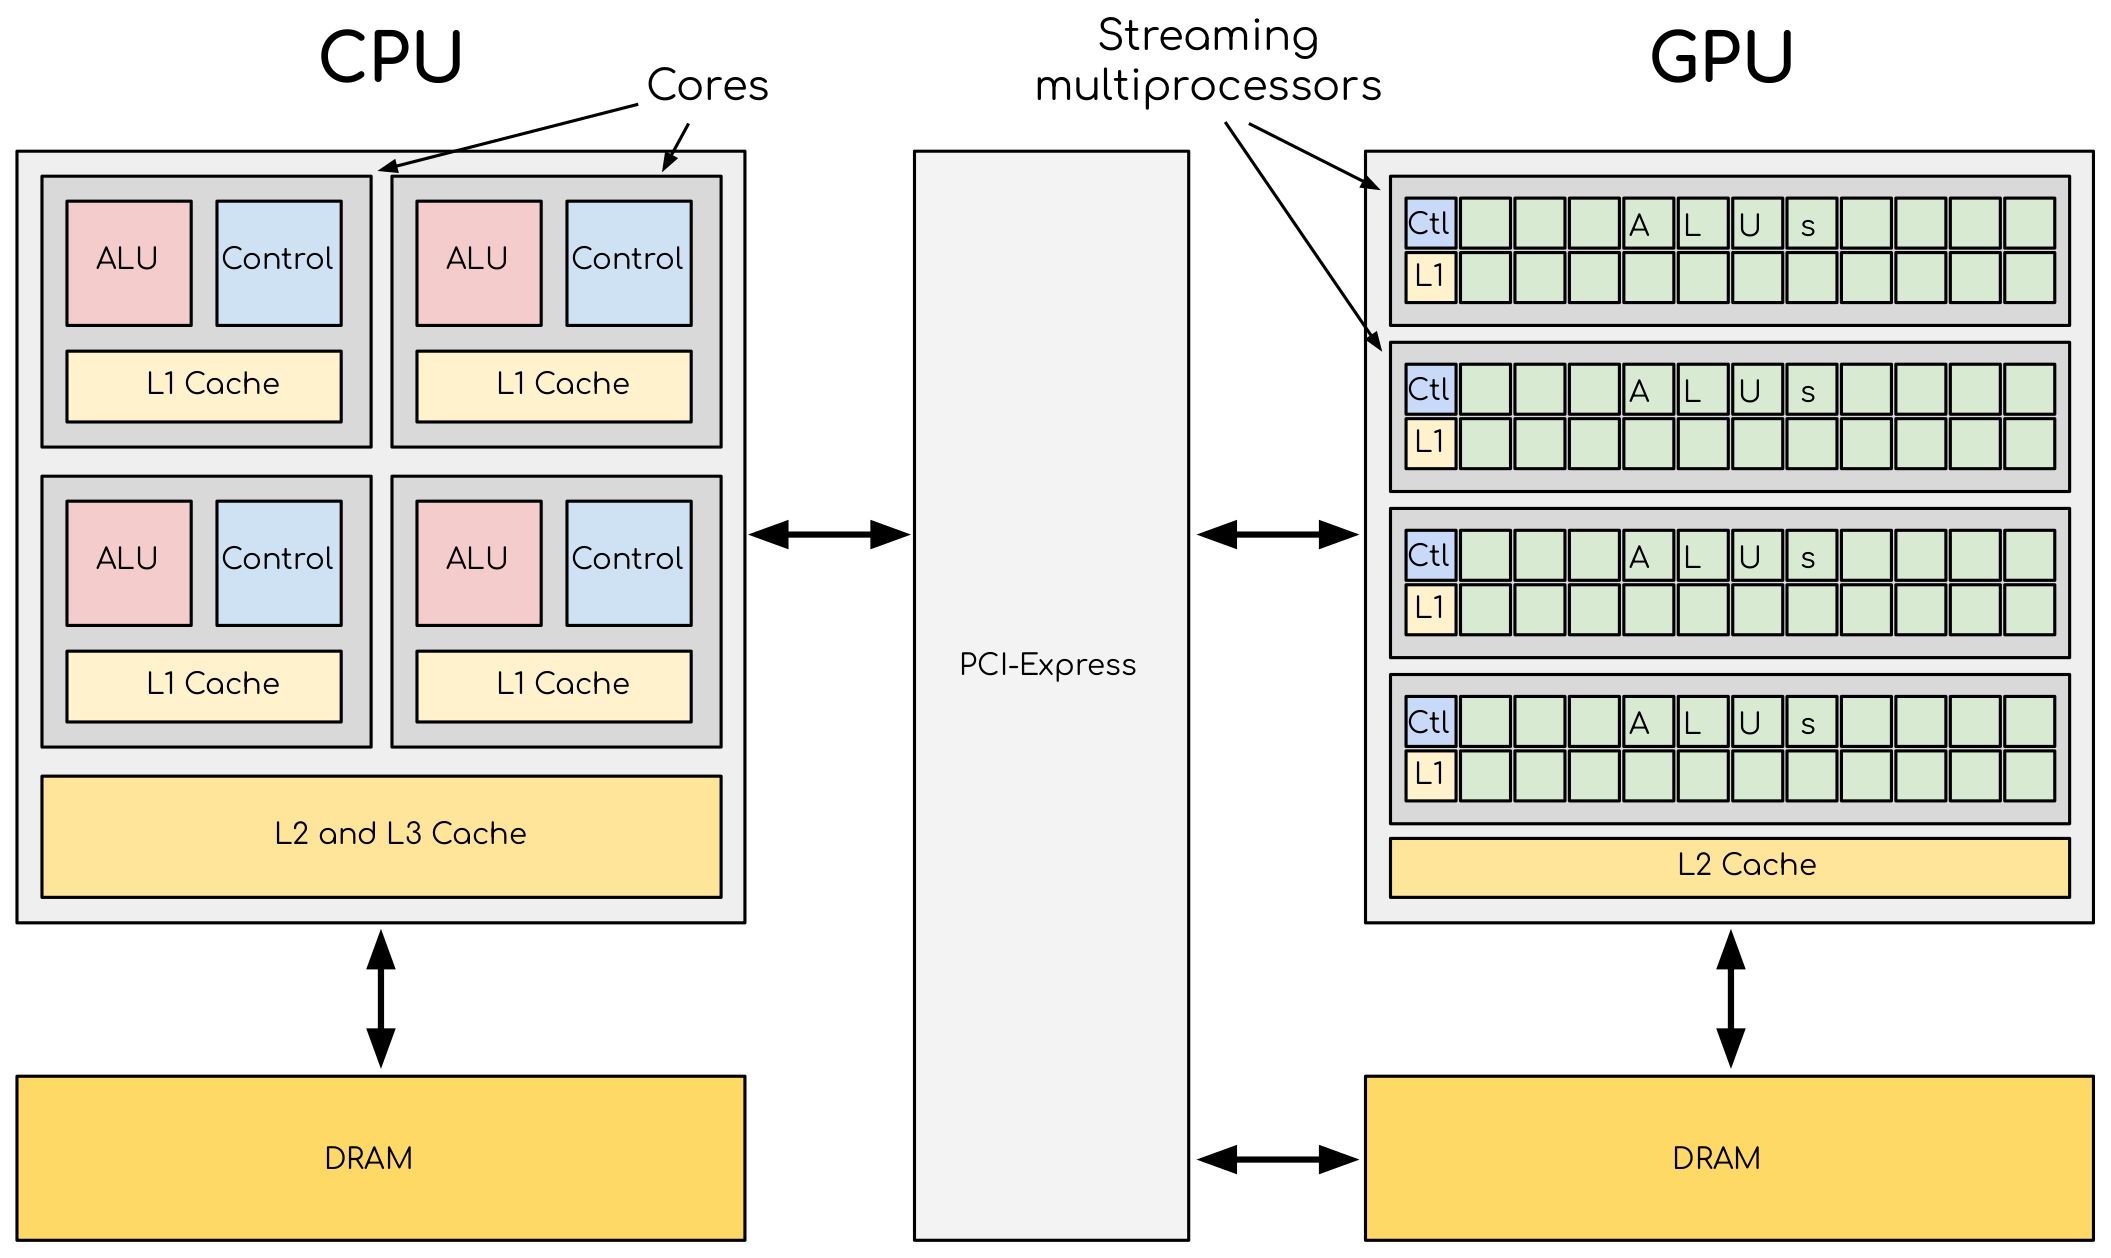
\includegraphics[width=0.8\textwidth]{images/estado_del_arte/cpu_vs_gpu.png}
   \caption[Comparativa de arquitecturas CPU y GPU]{Comparativa de arquitecturas CPU y GPU. Extraído de \cite{enccs_gpu_ecosystem}.}
   \label{fig:cpu_vs_gpu}
\end{figure}
La figura \ref{fig:cpu_vs_gpu} ilustra las diferencias arquitectónicas entre CPU y GPU. Las CPUs constan de un número reducido de núcleos (generalmente entre 4 y 64) optimizados para un alto rendimiento secuencial, donde cada núcleo dispone típicamente de caché y unidad de control privadas. En cambio, las \glspl{gpu} se basan en una arquitectura \textit{many-core}, integrando miles de núcleos más simples diseñados para el paralelismo masivo, aunque con menor rendimiento individual por núcleo. Estos núcleos de \glspl{gpu} suelen compartir recursos como la caché y las unidades de control, lo que posibilita empaquetar una mayor cantidad de unidades de procesamiento en el mismo chip y, consecuentemente, alcanzar una mayor densidad de cómputo.


NVIDIA ha sido una figura central en la evolución de la aceleración de IA, realizando contribuciones clave que han modelado el campo. Fue pionera en la computación de propósito general en \gls{gpu} con la introducción de CUDA en 2006. Esta plataforma permitió utilizar la masiva capacidad de procesamiento paralelo de las \gls{gpu} para tareas computacionales generales, extendiendo su uso más allá de los gráficos tradicionales. La programación de \gls{gpu} se realiza utilizando lenguajes y APIs especializadas como CUDA y OpenCL, que otorgan al desarrollador un control explícito sobre la distribución de datos y tareas entre los miles de núcleos disponibles.

El desarrollo eficaz en este paradigma requiere identificar y explotar el paralelismo inherente a los algoritmos, así como gestionar eficientemente la compleja jerarquía de memoria de la \gls{gpu}. Es crucial considerar la latencia significativamente mayor del acceso a la memoria global en comparación con memorias más rápidas pero de menor capacidad, como la memoria compartida local a un bloque de hilos.

Dada la complejidad de esta programación a bajo nivel, NVIDIA ha desarrollado un ecosistema de software robusto y optimizado para facilitar el desarrollo en IA. Este incluye bibliotecas fundamentales como cuDNN, específica para acelerar primitivas de redes neuronales profundas, y cuBLAS, para operaciones de álgebra lineal básica, ambas esenciales para el rendimiento. Además, es común recurrir a frameworks de alto nivel como PyTorch y TensorFlow. Estas librerías abstraen muchos detalles de la implementación en \gls{gpu}, utilizando las bibliotecas de NVIDIA subyacentes y simplificando enormemente el desarrollo de aplicaciones de inteligencia artificial.

En el frente del hardware, la compañía ha impulsado continuamente la innovación con el desarrollo de componentes especializados como los Tensor Cores, introducidos en la arquitectura Volta. Estos núcleos están diseñados específicamente para acelerar las operaciones matriciales intensivas (como multiplicaciones de matrices mixtas) que son omnipresentes en el entrenamiento e inferencia de modelos de IA. Como resultado de estas continuas innovaciones en hardware y la creación de un ecosistema de software integral, NVIDIA ha logrado establecer estándares de facto para la aceleración de IA, consolidándose como la plataforma preferida en una amplia gama de entornos, desde grandes centros de datos hasta sistemas embebidos con recursos limitados.


\subsection{Serie Jetson: Dispositivos de IA de bajo consumo} \label{sec:jetson}
La serie Jetson de NVIDIA constituye una familia de módulos computacionales diseñados específicamente para habilitar la inteligencia artificial y el aprendizaje profundo en dispositivos de borde (edge devices). Estos sistemas compactos y de bajo consumo son fundamentales para aplicaciones que requieren procesamiento local de datos con alta capacidad de cómputo.

El enfoque principal de la serie Jetson es la computación en el borde (edge computing), un paradigma que acerca el procesamiento de datos y la inteligencia artificial a la fuente donde se generan. Esto resulta crucial en aplicaciones donde la latencia, el ancho de banda limitado o la privacidad son factores críticos, ya que evita la necesidad de enviar grandes volúmenes de datos a la nube para su análisis. Los dispositivos Jetson están optimizados para operar bajo restricciones significativas de energía, tamaño y coste, características típicas de los entornos embebidos y de borde.

Cada módulo Jetson se basa en una arquitectura System-on-Chip (SoC), que integra múltiples componentes de procesamiento en un único circuito integrado. Esto incluye núcleos de CPU basados en la arquitectura ARM y potentes núcleos de \gls{gpu} NVIDIA con arquitecturas modernas. Además, algunos modelos de gama alta, como los Jetson AGX Orin y AGX Xavier utilizados en este trabajo, incorporan aceleradores de hardware dedicados conocidos como Deep Learning Accelerators (DLAs). Estas unidades especializadas están diseñadas para ejecutar operaciones de inferencia de redes neuronales de manera altamente eficiente en términos de rendimiento y consumo energético, liberando así la \gls{gpu} y la CPU para otras tareas. Esta integración heterogénea permite una alta eficiencia computacional y energética, reduce la huella física del sistema y simplifica el diseño de la placa portadora, resultando en soluciones más compactas y eficientes.

Un pilar fundamental del diseño de la serie Jetson es la optimización de la eficiencia energética. Estos dispositivos están diseñados para ofrecer un alto rendimiento computacional por cada vatio de energía consumido (TOPS/W), esencial para aplicaciones embebidas con fuentes de alimentación limitadas o restricciones térmicas. La capacidad de configurar diferentes perfiles de energía permite ajustar dinámicamente el equilibrio entre rendimiento y consumo.

Más allá del hardware, el valor de la plataforma Jetson reside en su ecosistema de software integral, proporcionado a través del NVIDIA JetPack SDK. Este paquete incluye el sistema operativo Linux optimizado (L4T), controladores, bibliotecas aceleradas por \gls{gpu} como CUDA, cuDNN y TensorRT, además de herramientas de desarrollo y documentación. Esta plataforma unificada simplifica el ciclo de desarrollo, desde la creación y entrenamiento de modelos hasta su optimización y despliegue en los dispositivos Jetson, acelerando la innovación.

\begin{table}[H]
   \centering
   \resizebox{\textwidth}{!}{%
   \begin{tabular}{l | c | c | c | c | c | c}
      \toprule
      Modelo & AI Performance & GPU & GPU Max Freq. & CPU & Memoria & DLAs \\
      Jetson AGX Orin & 275 TOPS & 2048-core Ampere, 64 Tensor Cores & 1.3 GHz & 12-core Cortex-A78AE, 3MB L2 + 6MB L3, 2.2 GHz & 64GB LPDDR5, 204.8GB/s & 2x NVDLA v2 \\ 
      Jetson Orin Nano & 67 TOPS & 1024-core Ampere, 32 Tensor Cores & 1020 MHz & 6-core Cortex-A78AE, 1.5MB L2 + 4MB L3, 1.7 GHz & 8GB LPDDR5, 102 GB/s & - \\ 
      Jetson AGX Xavier & 32 TOPS & 512-core Volta, 64 Tensor Cores & 1377 MHz & 8-core Carmel v8.2, 8MB L2 + 4MB L3, 2.2 GHz & 32GB LPDDR4x, 136.5GB/s & 2x NVDLA v1 \\
      \bottomrule
   \end{tabular}
   }
   \caption{Comparativa técnica entre diferentes modelos NVIDIA Jetson.}
   \label{tab:jetson_comparison}
\end{table}

La tabla \ref{tab:jetson_comparison}\cite{nvidia_jetson_modules} presenta una comparativa técnica entre diferentes modelos de la serie Jetson disponibles para la realización de este trabajo, incluyendo la presencia y tipo de DLAs. Cada modelo está diseñado para satisfacer diferentes necesidades y requisitos de rendimiento, lo que permite a los desarrolladores seleccionar el módulo más adecuado para su aplicación específica. Para este trabajo, se han utilizado los tres modelos de la tabla y se han comparado sus resultados.


\begin{figure}[H]
   \centering
   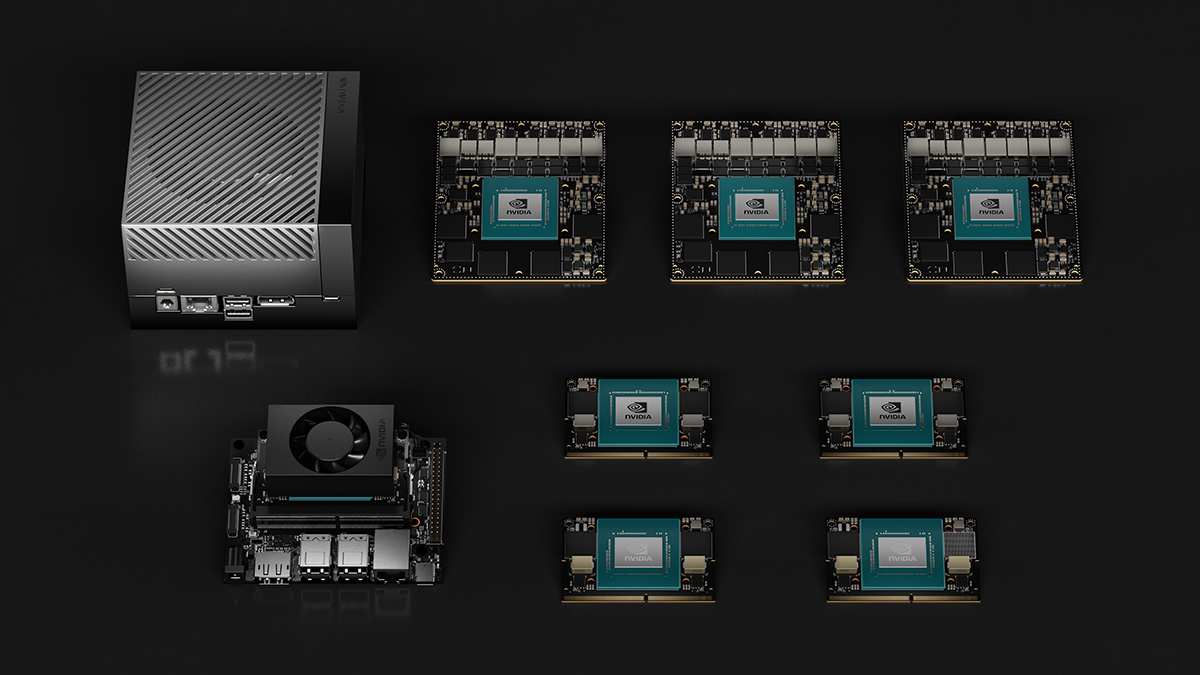
\includegraphics[width=0.8\textwidth]{images/estado_del_arte/jetson_family.png}
   \caption{Módulos Jetson de NVIDIA.}
   \label{fig:jetson_modules}
\end{figure}

\subsection{TensorRT} \label{sec:tensorrt}
NVIDIA TensorRT es un kit de desarrollo de software (SDK) integral diseñado específicamente para la optimización de modelos de aprendizaje profundo y la consecución de una inferencia de muy alto rendimiento en la amplia gama de hardware de NVIDIA, desde centros de datos hasta sistemas embebidos como la serie Jetson. Actúa como un potente compilador y motor de ejecución en tiempo real que transforma modelos previamente entrenados en versiones altamente eficientes, optimizadas para el despliegue en producción.

El objetivo principal de TensorRT es cerrar la brecha entre los frameworks de entrenamiento (como TensorFlow o PyTorch), que priorizan la flexibilidad y la facilidad de desarrollo, y los requisitos estrictos de las aplicaciones de inferencia en el mundo real, que demandan baja latencia, alto rendimiento (throughput) y eficiencia energética. Para lograr esto, TensorRT aplica una serie de optimizaciones sofisticadas durante una fase de compilación offline:

\begin{itemize}
   \item \textbf{Optimización del Grafo Computacional:} TensorRT analiza la estructura del modelo y realiza transformaciones significativas para mejorar la eficiencia. Esto incluye:
      \begin{itemize}
         \item \textit{Fusión de Capas (Layer Fusion):} Combina múltiples capas secuenciales (fusión vertical) o paralelas (fusión horizontal) en un único kernel optimizado. Por ejemplo, una secuencia de convolución, sesgo (bias) y activación (ReLU) puede fusionarse en una sola operación, reduciendo la sobrecarga de lanzamiento de kernels y el movimiento de datos en memoria.
         \item \textit{Eliminación de Capas:} Identifica y elimina capas que no son necesarias para la inferencia, como las capas de dropout.
         \item \textit{Fusión de Tensores (Tensor Fusion):} Combina operaciones que acceden a los mismos tensores para mejorar la localidad de los datos.
      \end{itemize}
   \item \textbf{Calibración y Cuantización de Precisión:} TensorRT ofrece un soporte robusto para reducir la precisión numérica de los pesos y activaciones del modelo. Puede convertir modelos de precisión completa (FP32) a precisiones más bajas como FP16 (media precisión), INT8 (enteros de 8 bits), o incluso formatos más recientes como FP8 o FP4 en hardware compatible. Esta reducción disminuye drásticamente el tamaño del modelo, el ancho de banda de memoria requerido y acelera el cómputo (especialmente en hardware con soporte nativo como los Tensor Cores), a menudo con una pérdida mínima o nula de precisión.
   \item \textbf{Selección Automática de Kernels (Kernel Auto-Tuning):} Durante la fase de construcción, TensorRT evalúa múltiples implementaciones (kernels) para cada operación en el hardware de destino específico y selecciona la más rápida disponible, considerando factores como el tamaño de los tensores y la precisión utilizada.
   \item \textbf{Gestión Dinámica de Memoria (Dynamic Tensor Memory):} Optimiza la asignación de memoria para los tensores intermedios, reutilizando la memoria siempre que sea posible para minimizar la huella de memoria global.
   \item \textbf{Ejecución Multi-Stream:} Facilita la ejecución concurrente de múltiples flujos de inferencia en la misma GPU, mejorando el rendimiento general del sistema.
\end{itemize}

\begin{figure}[H]
   \centering
   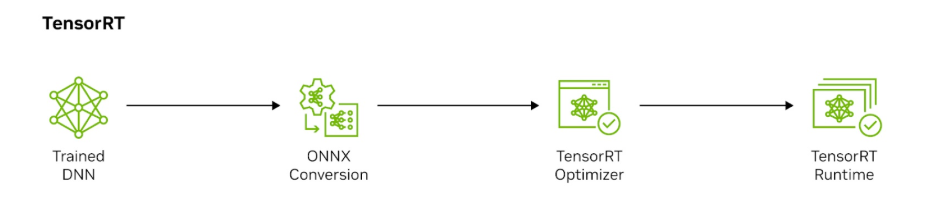
\includegraphics[width=0.8\textwidth]{images/estado_del_arte/TensorRT_pipeline.png}
   \caption{Ejemplo de flujo de trabajo de optimización con TensorRT.}
   \label{fig:tensorrt_architecture}
\end{figure}

El proceso típico de uso de TensorRT, como se ilustra esquemáticamente en la Figura~\ref{fig:tensorrt_architecture}, implica tomar un modelo entrenado (generalmente exportado a un formato intermedio como \gls{onnx}), utilizar el ``constructor'' (builder) de TensorRT para aplicar las optimizaciones y generar un ``motor'' (engine) de inferencia serializado y optimizado. Este motor es específico para el modelo, la precisión deseada y la plataforma hardware de destino (p. ej., un Jetson Orin Nano específico). Finalmente, el motor se carga en el ``tiempo de ejecución'' (runtime) de TensorRT para realizar inferencias rápidas y eficientes.

TensorRT se integra de forma nativa con los principales frameworks de aprendizaje profundo (TensorFlow, PyTorch) y soporta el formato de intercambio \gls{onnx}, lo que facilita la importación de modelos desde prácticamente cualquier framework de entrenamiento. Su capacidad para reducir significativamente la latencia y aumentar el rendimiento lo convierte en una herramienta esencial para desplegar modelos de IA en aplicaciones sensibles al tiempo real y en dispositivos con recursos limitados como los de la serie Jetson.



\section{Seguimiento de objetos en tiempo real} \label{sec:mot}
En esta sección se presentarán los conceptos básicos del seguimiento de objetos en tiempo real, se explicará el problema del seguimiento de objetos múltiples (MOT) y se presentarán los algoritmos más relevantes en este campo.

\subsection{Introducción al seguimiento de objetos} \label{sec:introduccion_seguimiento_objetos}
El seguimiento de objetos es un proceso que complementa la salida de los modelos de detección. Mientras que un modelo de detección opera sobre cada fotograma de forma independiente, identificando y localizando objetos como si fueran imágenes estáticas, el \gls{mot} actúa sobre estas detecciones para establecer una correspondencia temporal. La función esencial del \gls{mot} es asignar un identificador único a cada objeto detectado en un fotograma y mantener dicho identificador de manera consistente a lo largo de la secuencia de vídeo. Esto permite reconstruir las trayectorias de los objetos y analizar su comportamiento dinámico en la escena.

Para realizar este seguimiento, el \gls{mot} se basa en la información temporal y espacial de las detecciones. Utiliza técnicas de predicción y asociación para determinar la continuidad de los objetos a lo largo del tiempo, teniendo en cuenta factores como la posición, velocidad y apariencia de los objetos. El algoritmo utilizado para el seguimiento puede variar en complejidad, desde enfoques simples que utilizan filtros de Kalman para predecir la posición futura de un objeto, hasta métodos más avanzados que incorporan redes neuronales profundas para aprender características de apariencia y mejorar la robustez del seguimiento.


El filtro de Kalman es un algoritmo de estimación recursivo fundamental en el seguimiento de objetos. Funciona como un estimador óptimo para sistemas dinámicos lineales, permitiendo predecir el estado futuro de un objeto (como su posición y velocidad) a partir de una serie de mediciones ruidosas o incompletas a lo largo del tiempo. Su proceso se basa en dos etapas cíclicas:
\begin{itemize}
   \item \textbf{Predicción:} Utiliza un modelo dinámico del movimiento esperado del objeto para estimar su estado en el siguiente instante de tiempo.
   \item \textbf{Actualización:} Incorpora la nueva medición (detección) obtenida en ese instante para corregir la predicción inicial, ponderando la información del modelo y la medición según su incertidumbre asociada.
\end{itemize}
Este ciclo permite al filtro refinar continuamente la estimación del estado del objeto, suavizar las trayectorias y manejar eficazmente el ruido inherente a las mediciones del detector. Es una herramienta clave para mantener la identidad de los objetos entre fotogramas, especialmente cuando las detecciones son intermitentes o imprecisas.



\begin{figure}[H]
   \centering
   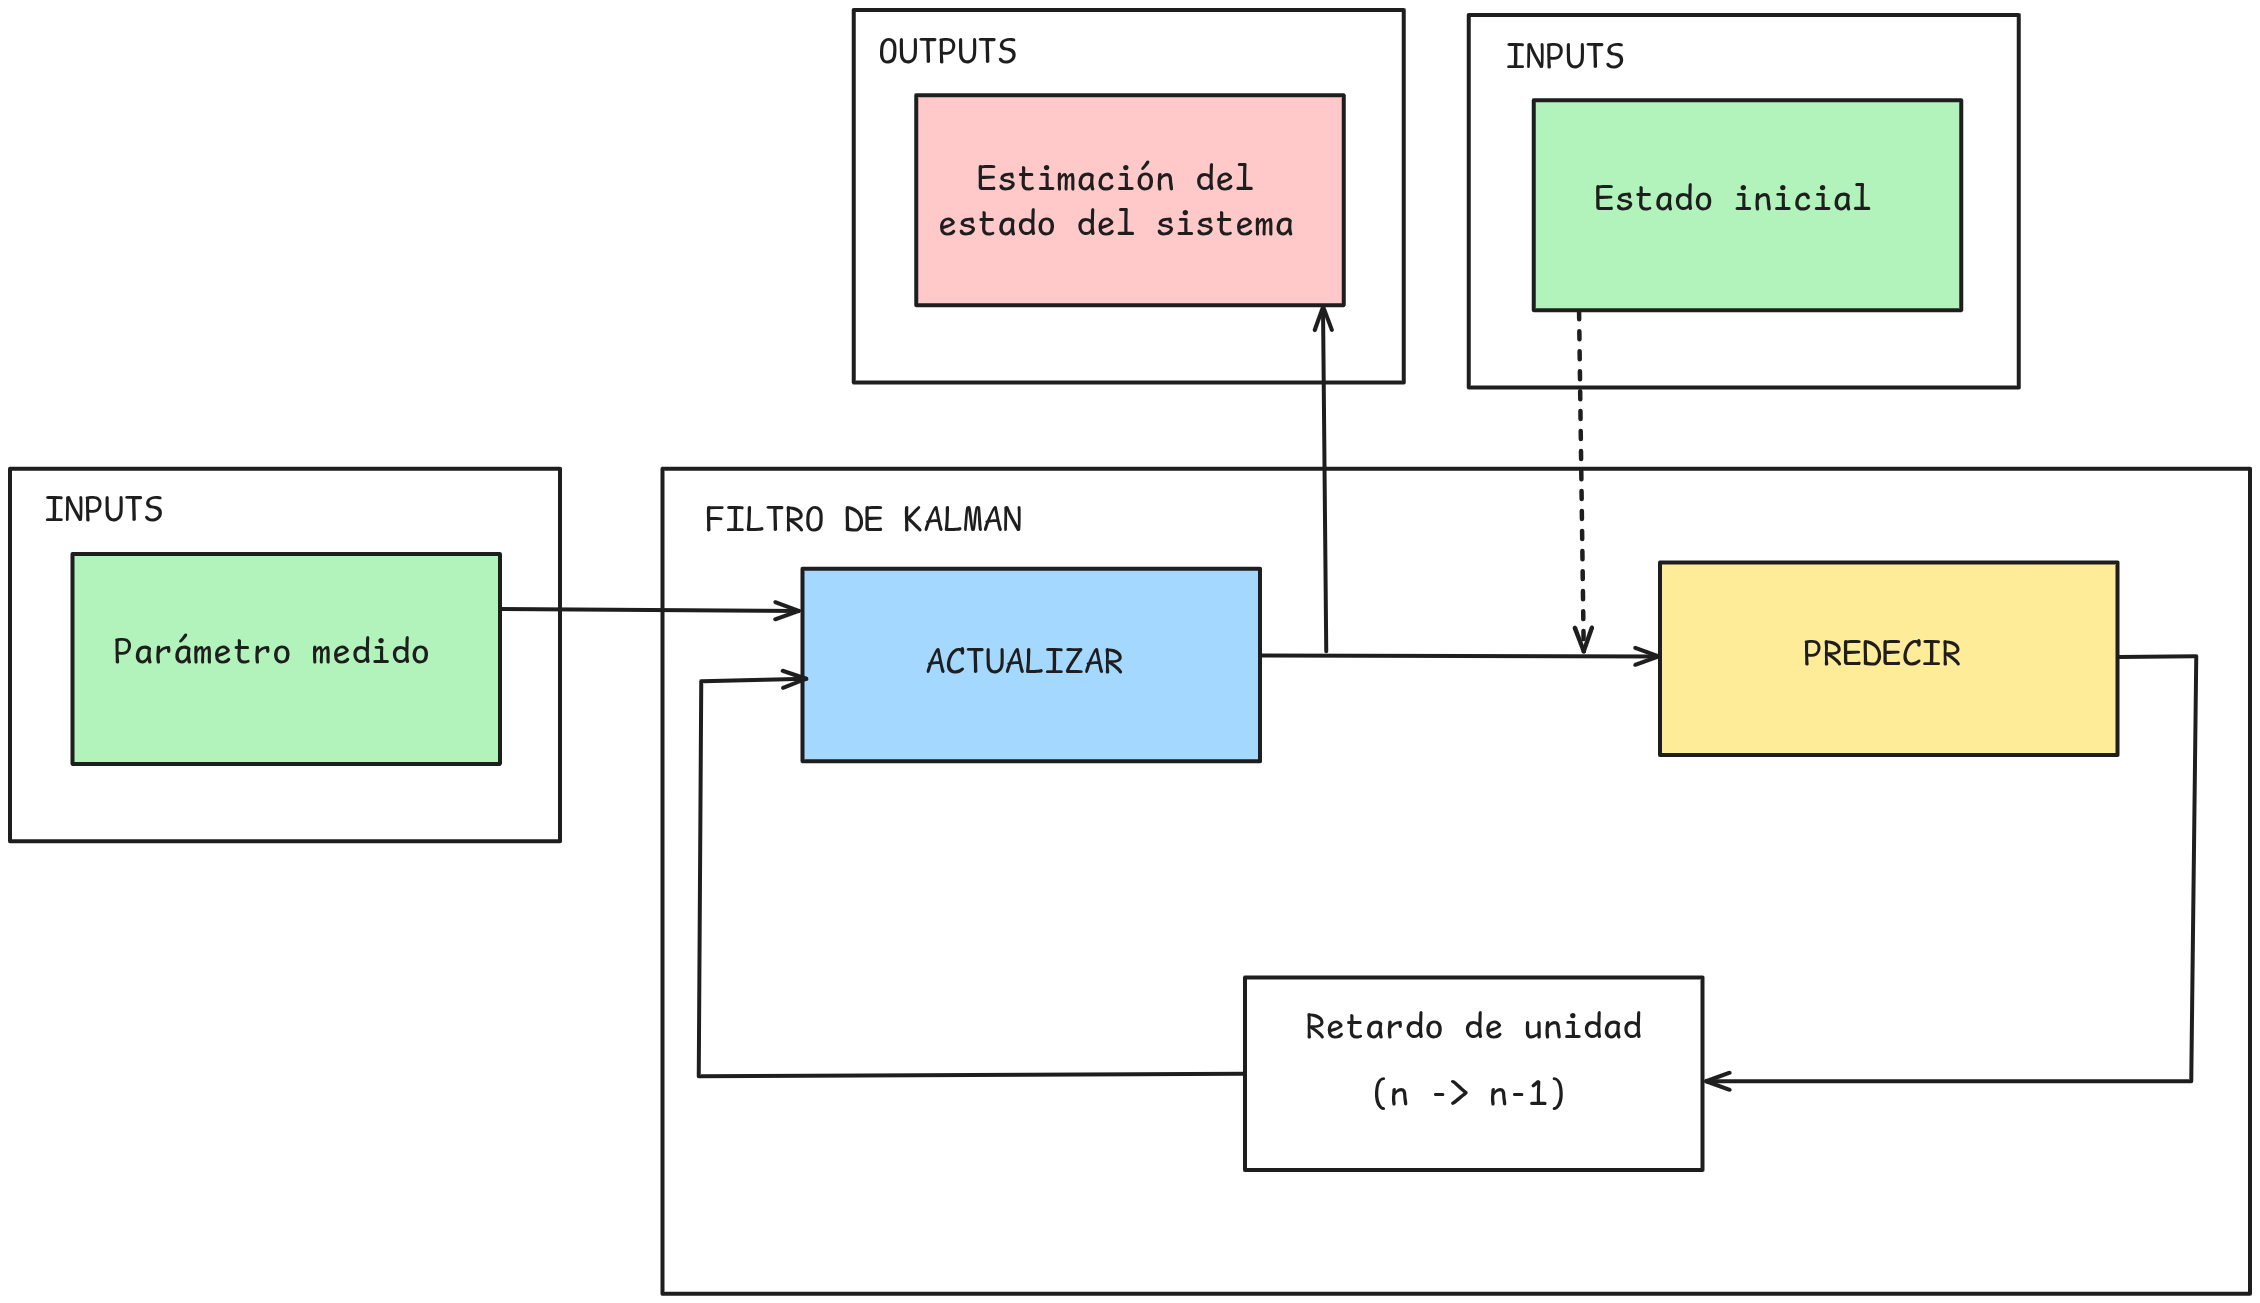
\includegraphics[width=0.8\textwidth]{images/estado_del_arte/filtro_de_kalman.png}
   \caption{Diagrama de flujo del filtro de Kalman.}
   \label{fig:filtro_de_kalman}
\end{figure}

La Figura ~\ref{fig:filtro_de_kalman} representa el funcionamiento de un filtro de Kalman, un algoritmo muy utilizado para estimar el estado de un sistema dinámico en presencia de ruido e incertidumbre. A continuación se explica cada bloque:

\begin{itemize}
   \item \textbf{INPUTS: Parámetro medido}
   Este bloque representa las mediciones que se obtienen del sistema. Estas mediciones contienen errores (ruido), por lo que no se usan directamente, sino que se pasan al filtro para su procesamiento.

   \item \textbf{INPUTS: Estado inicial}
   Proporciona una estimación inicial del estado del sistema y su incertidumbre asociada. Esta información se utiliza para arrancar el filtro de Kalman.

   \item \textbf{ACTUALIZAR}
   Este es uno de los dos pasos principales del filtro de Kalman. Combina la predicción previa con la medición actual para actualizar la estimación del estado del sistema y ajusta la incertidumbre de esa estimación.

   \item \textbf{PREDECIR}
   El otro paso clave del filtro utiliza el modelo del sistema para predecir el siguiente estado y su incertidumbre, basándose en la estimación anterior y considerando el retardo de una unidad.

   \item \textbf{Retardo de unidad (\(n \rightarrow n{-}1\))}
   Este bloque representa el almacenamiento del estado estimado en el instante anterior para ser utilizado en la siguiente predicción.

   \item \textbf{OUTPUTS: Estimación del estado del sistema}
   Este es el resultado final del filtro: una estimación refinada del estado actual del sistema, que es más precisa que la simple medición directa.
\end{itemize}

En conjunto, el filtro de Kalman realiza un ciclo continuo de predicción y corrección, usando tanto el modelo del sistema como las mediciones reales, para obtener una estimación óptima del estado.



% \begin{itemize}
%    \item \textbf{Introducción al Seguimiento de Objetos Múltiples (MOT):} Definición del problema, importancia y aplicaciones principales.
%    \item \textbf{Desafíos del MOT:} Se discutirán las dificultades inherentes al seguimiento, como oclusiones, cambios de apariencia, interacciones entre objetos, entradas y salidas de la escena, y errores de detección.
%    \item \textbf{Paradigma Tracking-by-Detection:} Explicación del enfoque dominante en MOT, que consiste en detectar objetos en cada fotograma y luego asociar estas detecciones a lo largo del tiempo para formar trayectorias.
%    \item \textbf{Filtro de Kalman:} Descripción de sus fundamentos matemáticos como estimador óptimo para sistemas lineales y su aplicación para predecir la posición futura de los objetos y suavizar las trayectorias, manejando la incertidumbre en las mediciones.
%    \item \textbf{Asociación de Datos:} Técnicas para vincular las detecciones actuales con las trayectorias existentes, como el algoritmo Húngaro basado en métricas de similitud (IoU, apariencia).
%    \item \textbf{Algoritmos Clásicos:}
%       \begin{itemize}
%          \item \textbf{SORT (Simple Online and Realtime Tracking):} Enfoque basado principalmente en el Filtro de Kalman y la métrica IoU para la asociación, destacando por su simplicidad y velocidad.
%          \item \textbf{DeepSORT (Deep Simple Online and Realtime Tracking):} Extensión de SORT que incorpora características de apariencia extraídas mediante redes profundas para mejorar la robustez frente a oclusiones prolongadas.
%       \end{itemize}
%    \item \textbf{Algoritmos Modernos - BYTETrack:} Presentación de BYTETrack, que mejora la gestión de detecciones de baja confianza para manejar mejor las oclusiones y reducir la fragmentación de trayectorias, separando las detecciones de alta y baja confianza en el proceso de asociación.
%    \item \textbf{Métricas de Evaluación para MOT:} Introducción a las métricas estándar para evaluar el rendimiento de los algoritmos de seguimiento, como MOTA (Multiple Object Tracking Accuracy), MOTP (Multiple Object Tracking Precision), IDF1, HOTA (Higher Order Tracking Accuracy), entre otras.
% \end{itemize}


\subsection{BYTETrack}\label{sec:bytetrack}

BYTETrack \cite{zhang2022bytetrackmultiobjecttrackingassociating} es un algoritmo avanzado de Seguimiento de Objetos Múltiples (MOT) que se inscribe dentro del paradigma de seguimiento por detección (\textit{tracking-by-detection}). Este paradigma consiste en detectar objetos en cada fotograma de forma independiente y luego asociar estas detecciones a lo largo del tiempo para construir trayectorias coherentes. La innovación fundamental de BYTETrack reside en su novedoso método de asociación de datos, denominado BYTE, que aborda explícitamente un problema común en MOT: el manejo de detecciones con baja puntuación de confianza.

Mientras que la mayoría de los algoritmos de seguimiento descartan las detecciones por debajo de un cierto umbral de confianza para evitar la introducción de falsos positivos, BYTETrack reconoce que estas detecciones de baja confianza a menudo corresponden a objetos reales que están parcialmente ocluidos o cuya apariencia ha cambiado temporalmente. Descartarlas puede llevar a la pérdida de trayectorias y a una menor precisión general del seguimiento. Esta estrategia de asociación en dos pasos permite a BYTETrack recuperar objetos reales incluso cuando la confianza del detector disminuye debido a oclusiones o desenfoque, manteniendo la continuidad de las trayectorias. Al separar claramente las detecciones de alta y baja confianza y utilizarlas de manera diferenciada en el proceso de asociación, BYTETrack logra una notable mejora en la robustez del seguimiento, reduce significativamente la fragmentación de las trayectorias (medida por métricas como IDF1) y maneja eficazmente las variaciones en la calidad de las detecciones, todo ello manteniendo una alta eficiencia computacional.

\begin{figure}[H]
   \centering
   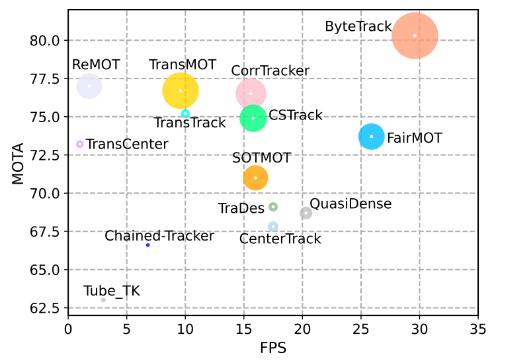
\includegraphics[width=0.5\textwidth]{images/estado_del_arte/BYTETrack_MOTA.png}
   \caption[Comparativa de rendimiento de BYTETrack con otros algoritmos de seguimiento]{Comparativa de rendimiento de BYTETrack con otros algoritmos de seguimiento. Extraído de \cite[fig. 1, p.~1]{zhang2022bytetrackmultiobjecttrackingassociating}.}
   \label{fig:bytetrack_mota}
\end{figure}

La Figura \ref{fig:bytetrack_mota} presenta una comparativa de rendimiento que evidencia la superioridad de BYTETrack frente a otros algoritmos de seguimiento, según los resultados publicados en \cite{zhang2022bytetrackmultiobjecttrackingassociating}. Como se observa, BYTETrack no solo alcanza una mayor precisión, medida por la métrica MOTA (Multiple Object Tracking Accuracy), sino que también demuestra una velocidad de procesamiento superior. Estas características lo posicionan como una solución particularmente eficaz y atractiva para aplicaciones que demandan seguimiento de objetos en tiempo real.

\begin{figure}[H]

   \centering
   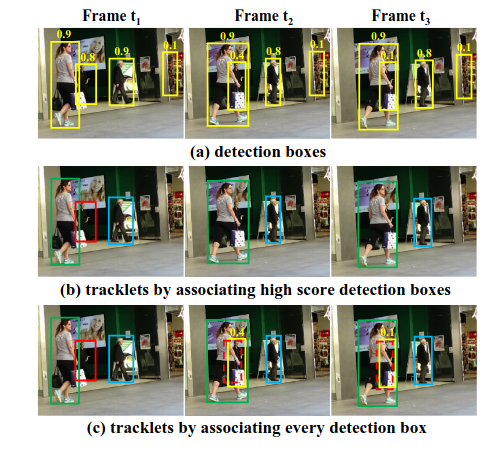
\includegraphics[width=0.5\textwidth]{images/estado_del_arte/BYTETrack_deteccion.png}
   \caption[Ejemplo de detección y seguimiento de objetos utilizando BYTETrack]{Ejemplo de detección y seguimiento de objetos utilizando BYTETrack. Extraído de \cite[fig. 2, p.~2]{zhang2022bytetrackmultiobjecttrackingassociating}.}
   \label{fig:bytetrack_deteccion}
\end{figure}

La Figura \ref{fig:bytetrack_deteccion} ilustra el proceso de BYTETrack a través de tres fotogramas consecutivos ($\tau_1$, $\tau_2$, $\tau_3$) de una secuencia de vídeo. En (a), se observan las detecciones iniciales que superan un umbral de confianza (p. ej., 0.5). La sección (b) muestra las trayectorias generadas al asociar exclusivamente las detecciones de alta confianza. Por el contrario, (c) presenta el resultado final de BYTETrack, que integra también las detecciones de baja confianza en el proceso de asociación. Esta comparación evidencia cómo la estrategia de BYTETrack permite mantener la continuidad de las trayectorias frente a desafíos como oclusiones parciales y variaciones en la confianza de las detecciones, logrando así una representación más precisa y robusta del movimiento de los objetos en el tiempo.



El funcionamiento del algoritmo BYTETrack es el siguiente:

\textbf{Input:} Una secuencia de vídeo $V$, un detector de objetos $Det$, y un umbral de confianza de detección $\tau$.

\textbf{Output:} Las trayectorias $\mathcal{T}$ de los objetos detectados en el vídeo.

\begin{enumerate}
   \item \textbf{Inicialización:} Se inicializa el conjunto de trayectorias $\mathcal{T}$ como vacío.
   \item \textbf{Procesamiento por fotograma:} Para cada fotograma $f_k$ en la secuencia de vídeo $V$:
   { % Start a group to keep the redefinition local
   \renewcommand{\theenumii}{\theenumi.\arabic{enumii}} % Change numbering to 1.1, 1.2, etc.
   \renewcommand{\labelenumii}{\theenumii.} % Add trailing dot to the label
   \begin{enumerate}
      \item \textbf{Detección:} Se utiliza el detector $Det$ para obtener las cajas delimitadoras y sus puntuaciones de confianza para el fotograma $f_k$, resultando en un conjunto de detecciones $\mathcal{D}_k$.
      \item \textbf{Separación de detecciones:} Se inicializan dos conjuntos vacíos: $\mathcal{D}_{high}$ para detecciones de alta confianza y $\mathcal{D}_{low}$ para detecciones de baja confianza. Se itera sobre cada detección $d$ en $\mathcal{D}_k$:
      \begin{itemize}
         \item Si la puntuación $d.score$ es mayor que el umbral $\tau$, la detección $d$ se añade a $\mathcal{D}_{high}$.
         \item En caso contrario, la detección $d$ se añade a $\mathcal{D}_{low}$.
      \end{itemize}
      \item \textbf{Predicción de trayectorias:} Para cada trayectoria existente $t$ en $\mathcal{T}$, se predice su nueva ubicación utilizando un Filtro de Kalman.
      \item \textbf{Primera asociación:} Se asocian las trayectorias $\mathcal{T}$ con las detecciones de alta confianza $\mathcal{D}_{high}$ utilizando el \textit{Hungarian alogorithm}\cite{kuhn1955hungarian} con la métrica de similitud IoU (Intersection over Union). Las detecciones no asociadas se guardan en $\mathcal{D}_{remain}$ y las trayectorias no asociadas en $\mathcal{T}_{remain}$.
      \item \textbf{Segunda asociación:} Se asocian las trayectorias restantes $\mathcal{T}_{remain}$ con las detecciones de baja confianza $\mathcal{D}_{low}$ utilizando otra métrica de similitud (Similarity\#2, usualmente IoU). Las trayectorias que siguen sin asociarse se guardan en $\mathcal{T}_{re-remain}$. Solo se asocian detecciones de baja confianza a trayectorias que no pudieron ser asociadas con detecciones de alta confianza.
      \item \textbf{Eliminación de trayectorias no asociadas:} Se eliminan de $\mathcal{T}$ las trayectorias que quedaron en $\mathcal{T}_{re-remain}$ (aquellas que no se pudieron asociar ni en la primera ni en la segunda etapa) si han permanecido sin asociar durante un número determinado de fotogramas (definido por el parámetro track\_buffer).
      \item \textbf{Inicialización de nuevas trayectorias:} Se itera sobre las detecciones de alta confianza que no fueron asociadas ($\mathcal{D}_{remain}$). Cada una de estas detecciones se considera el inicio de una nueva trayectoria y se añade al conjunto $\mathcal{T}$.
   \end{enumerate}
   } % End the group
   \item \textbf{Retorno:} Una vez procesados todos los fotogramas, se devuelve el conjunto final de trayectorias $\mathcal{T}$.
\end{enumerate}


Con todo esto, BYTETrack logra un seguimiento robusto y preciso de múltiples objetos en movimiento, incluso en condiciones desafiantes como oclusiones parciales y cambios de apariencia. Su enfoque innovador para manejar detecciones de baja confianza lo distingue de otros algoritmos de seguimiento y lo convierte en una opción atractiva para aplicaciones en tiempo real.


\subsection{Métricas de evaluación en MOT} \label{sec:metricas_mot}

Las métricas de evaluación son fundamentales para medir el rendimiento de los algoritmos de seguimiento de objetos múltiples (MOT). Estas métricas permiten cuantificar la precisión y la robustez del seguimiento, facilitando la comparación entre diferentes enfoques y configuraciones.

En el contexto de MOT, los errores pueden clasificarse en tres categorías principales:

\begin{itemize}
   \item \textbf{Errores de detección:} Ocurren cuando el sistema predice detecciones que no existen en la verdad de referencia, o cuando falla en predecir detecciones que sí están presentes en la verdad fundamental. Estos corresponden a los Falsos Positivos (FP) y Falsos Negativos (FN) respectivamente.
   
   \item \textbf{Errores de asociación:} Se producen cuando el sistema asigna el mismo ID de predicción (prID) a dos detecciones que tienen diferentes IDs en la verdad de referencia (gtID), o cuando asigna diferentes prIDs a dos detecciones que deberían tener el mismo gtID. El caso más común es el Cambio de Identidad (IDSW - IDentity SWitch).
   
   \item \textbf{Errores de localización:} Ocurren cuando las detecciones predichas (prDets) no están perfectamente alineadas espacialmente con las detecciones de la verdad de referencia (gtDets). La calidad de esta alineación se mide típicamente con la métrica IoU (Intersection over Union).
\end{itemize}

A continuación se presentan las métricas más relevantes en este campo, que cuantifican estos errores de diversas maneras:

\begin{itemize}
   \item \textbf{MOTA (Multiple Object Tracking Accuracy):} Es una de las métricas más consolidadas y ampliamente utilizadas para evaluar el rendimiento general de un algoritmo MOT. MOTA agrega tres tipos de errores principales que pueden ocurrir durante el seguimiento:
   \begin{itemize}
     \item Falsos Negativos (FN): Objetos reales presentes en la escena que el algoritmo de seguimiento no detecta o no sigue.
     \item Falsos Positivos (FP): Detecciones o trayectorias generadas por el algoritmo de seguimiento que no corresponden a ningún objeto real.
     \item Cambios de Identidad (IDSW - IDentity SWitches): Ocurren cuando un objeto que ya está siendo seguido se le asigna incorrectamente un nuevo identificador, o cuando se intercambian los identificadores entre dos objetos seguidos.
   \end{itemize}
   La fórmula es:
   \begin{equation}
   MOTA = 1 - \frac{\sum_{t} (FN_t + FP_t + IDSW_t)}{\sum_{t} GT_t}
   \end{equation}
   donde \(FN_t\), \(FP_t\), e \(IDSW_t\) son el número de falsos negativos, falsos positivos y cambios de identidad en el fotograma \(t\), respectivamente. \(GT_t\) es el número total de objetos reales (verdad de referencia) en el fotograma \(t\). El sumatorio se realiza sobre todos los fotogramas de la secuencia.
   Un valor de MOTA más alto indica un mejor rendimiento, con un máximo teórico de 1 (o 100\%). Sin embargo, MOTA puede ser negativo si el número de errores supera el número de objetos reales. Aunque es una métrica integral, tiende a dar más peso a la precisión de la detección que a la consistencia de la identidad a largo plazo.

   \item \textbf{MOTP (Multiple Object Tracking Precision):} Esta métrica evalúa la precisión de la localización de los objetos a lo largo del tiempo. Se calcula como la media de las distancias entre las cajas delimitadoras predichas y las cajas delimitadoras reales (verdad de referencia) para todas las asociaciones correctas. Matemáticamente, se expresa como:
   \begin{equation}
   MOTP = \frac{\sum_{t,i} d_{t,i}}{\sum_{t} c_t}
   \end{equation}
   donde $d_{t,i}$ es la distancia (generalmente IoU) entre la predicción y la verdad de referencia para el objeto $i$ en el fotograma $t$, y $c_t$ es el número total de asociaciones correctas en el fotograma $t$. Un valor de MOTP más alto indica una mayor precisión en la localización de los objetos. A diferencia de MOTA, MOTP no penaliza los errores de identidad, sino que se centra exclusivamente en qué tan precisas son las localizaciones de los objetos cuando se asocian correctamente.

   \item \textbf{IDF1 (ID F1 Score):} Esta métrica se centra específicamente en la capacidad del algoritmo de seguimiento para mantener correctamente la identidad de los objetos a lo largo del tiempo. Es la media armónica de la Precisión de ID (IDP) y el Recall de ID (IDR).
   \begin{itemize}
     \item IDP (ID Precision): Proporción de detecciones correctamente asignadas a una trayectoria (ID) respecto al total de detecciones asignadas.
     \item IDR (ID Recall): Proporción de objetos reales correctamente identificados y seguidos a lo largo de su trayectoria respecto al total de objetos reales.
   \end{itemize}
   La fórmula es:
   \begin{equation}
   IDF1 = \frac{2 \cdot IDTP}{2 \cdot IDTP + IDFP + IDFN}
   \end{equation}
   donde \(IDTP\) (ID True Positives) son los verdaderos positivos en términos de asignación de identidad correcta a lo largo de las trayectorias, \(IDFP\) (ID False Positives) son las asignaciones de identidad incorrectas, y \(IDFN\) (ID False Negatives) son las identidades de objetos reales que no fueron correctamente mantenidas. Un valor de IDF1 más alto (hasta 1 o 100\%) indica una mejor consistencia en el seguimiento de la identidad. Es particularmente útil para evaluar el rendimiento en escenarios con oclusiones prolongadas o interacciones complejas entre objetos.

   \item \textbf{HOTA (Higher Order Tracking Accuracy):} Es una métrica más reciente diseñada para proporcionar una evaluación más equilibrada y completa del rendimiento del MOT. HOTA descompone explícitamente el rendimiento en precisión de detección, precisión de asociación y precisión de localización. Se calcula como la media geométrica de la Precisión de Detección (DetA) y la Precisión de Asociación (AssA), donde cada una de estas componentes considera la precisión de localización (IoU).
   \begin{equation}
   HOTA = \sqrt{DetA \cdot AssA}
   \end{equation}
   \begin{itemize}
     \item DetA (Detection Accuracy): Mide qué tan bien se detectan los objetos, promediado sobre diferentes umbrales de IoU.
     \item AssA (Association Accuracy): Mide qué tan bien se asocian las detecciones correctas para formar trayectorias consistentes, también promediado sobre umbrales de IoU.
   \end{itemize}
   HOTA varía entre 0 y 1 (o 0\% y 100\%), donde valores más altos indican un mejor rendimiento. Se considera que HOTA ofrece una visión más matizada que MOTA, ya que penaliza de forma más equilibrada los diferentes tipos de errores y es sensible a la calidad de la localización.


\end{itemize}

% \section{Slicing Aided Hyper Inference}
% Explicación de la técnica de Slicing Aided Hyper Inference, como se utiliza para mejorar la precisión de los modelos de detección de objetos y como se aplica en este trabajo.




\chapter{Diseño e implementación de la solución}\label{chap:diseno_e_implementacion}

En este capítulo se abordará en profundidad el diseño y la implementación del sistema de visión artificial propuesto. Se iniciará con un análisis detallado del problema a resolver, definiendo los desafíos inherentes a la detección y seguimiento de objetos en movimiento y los requisitos específicos del sistema, como la operación en tiempo real. A continuación, se describirá el proceso de entrenamiento de los modelos de detección de objetos, la metodología para la creación y anotación del conjunto de datos de canicas, y los parámetros de entrenamiento utilizados. Posteriormente, se presentará una descripción global del sistema, detallando su arquitectura modular y el flujo de datos entre sus componentes. Se profundizará en el diseño específico de cada una de las etapas que conforman el sistema: la captura de imágenes, la inferencia del modelo de detección, el seguimiento de los objetos mediante el algoritmo BYTETrack y la escritura de los resultados. Finalmente, se explorarán y justificarán las diversas estrategias de segmentación del sistema (secuencial, basada en hilos, basada en procesos, y optimizaciones con memoria compartida o aceleración por hardware específico) que se han considerado e implementado con el objetivo de optimizar el rendimiento y la eficiencia del procesamiento en la plataforma NVIDIA Jetson.



\section{Análisis del problema}\label{sec:analisis_problema}

El desafío central abordado en este trabajo consiste en el desarrollo y la implementación de un sistema de visión artificial capaz de realizar el seguimiento de múltiples objetos en movimiento en tiempo real y poder detectar sus posibles defectos. Este sistema se fundamenta en la utilización de la plataforma de hardware NVIDIA Jetson, reconocida por su capacidad para ejecutar tareas de inteligencia artificial de manera eficiente en términos energéticos y computacionales. La tarea principal del sistema es procesar una secuencia de vídeo, identificar los objetos presentes en cada fotograma mediante un modelo de detección de objetos basado en redes neuronales profundas, y posteriormente, aplicar un algoritmo de seguimiento para mantener la identidad de cada objeto a lo largo del tiempo, reconstruyendo así sus trayectorias.

Un requisito fundamental y crítico para la viabilidad del sistema es su capacidad para operar en tiempo real. Esto impone una restricción estricta sobre la velocidad de procesamiento: el tiempo total necesario para analizar un fotograma individual, incluyendo tanto la detección como el seguimiento de los objetos, debe ser inferior al intervalo de tiempo que transcurre entre fotogramas consecutivos en la secuencia de vídeo. Por ejemplo, para un vídeo a 30 fotogramas por segundo, el procesamiento completo de cada fotograma debe completarse en menos de 33.3 milisegundos. Cumplir con esta exigencia es particularmente desafiante dadas las limitaciones inherentes de los dispositivos embebidos como los de la serie Jetson, que, aunque potentes, disponen de recursos computacionales y memoria significativamente menores en comparación con sistemas de escritorio o servidores.

Dada la dificultad de acceder a un entorno industrial real para llevar a cabo las pruebas experimentales —como podría ser una línea de producción activa en una fábrica de conservas, una planta de ensamblaje de componentes electrónicos o una instalación de procesamiento de alimentos—, se optó por utilizar un entorno simulado controlado. Este entorno sustituye los objetos industriales por elementos más manejables y disponibles, específicamente, canicas de diversos colores. Estas canicas, al moverse sobre una superficie o cinta transportadora improvisada, simulan el flujo de objetos que se encontraría en una línea de producción. La utilización de este entorno simulado ofrece ventajas significativas para la fase de desarrollo y evaluación: permite realizar pruebas de manera sistemática y repetible, facilita la variación controlada de parámetros (como la velocidad de los objetos, la iluminación o la densidad de objetos) y posibilita la obtención de datos cuantitativos precisos sobre el rendimiento del sistema en diferentes condiciones. Aunque este entorno simplifica la complejidad del mundo real, los resultados y las conclusiones obtenidas proporcionan una base sólida y pueden ser extrapolados, con las debidas consideraciones, para predecir el comportamiento y la eficacia del sistema en escenarios industriales auténticos.

\begin{figure}[H]
   \centering
   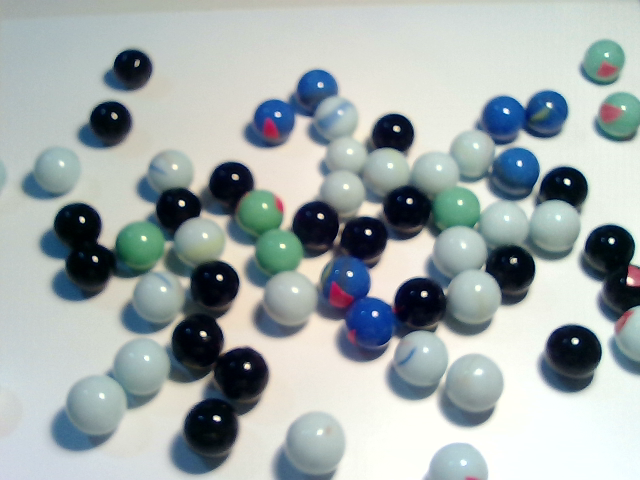
\includegraphics[width=0.6\textwidth]{images/diseno_e_implementacion/ejemplo_canicas.png}
   \caption{Ejemplo de entorno simulado con canicas.}
   \label{fig:entorno_simulado}
\end{figure}

Para las pruebas experimentales, se configuró un entorno simulado como el ilustrado en la Figura \ref{fig:entorno_simulado}. Este entorno utiliza canicas de cuatro colores distintos (blanco, negro, azul y verde). Con el objetivo de simular la detección de anomalías, se consideraron tanto canicas sin defectos como canicas con defectos para cada uno de los colores. Como defecto, se añadió una mancha de un color diferente al de la canica, presentando diversas formas. Esta distinción duplica el número total de clases que el sistema debe identificar, alcanzando un total de ocho categorías (cuatro colores sin defecto y cuatro colores con defecto).


\section{Entrenamiento de los modelos} \label{sec:entrenamiento_modelo}

La selección y el entrenamiento de los modelos de detección de objetos constituyen una fase crítica en el desarrollo del sistema propuesto, ya que de ello dependen directamente la precisión y la robustez del sistema final.
Tras un análisis comparativo, se optó por los detectores de una etapa frente a los de dos etapas, dada su superior eficiencia para aplicaciones que exigen procesamiento en tiempo real. Dentro de esta categoría, se seleccionó la familia de modelos YOLO. Esta elección se fundamenta en su reconocido equilibrio entre velocidad de inferencia y precisión, así como en la disponibilidad de un robusto ecosistema de herramientas que facilitan tanto el entrenamiento como el despliegue. Alternativas como SSD, si bien competentes, no ofrecían el mismo conjunto de ventajas en términos de comunidad de soporte y facilidad de integración para los fines de este proyecto.

Como modelos pertenecientes a la familia de arquitecturas YOLO, se han seleccionado diversas variantes para una evaluación exhaustiva: YOLOv5 (específicamente las versiones 'n' y 'm'), YOLOv8 (también en sus variantes 'n' y 's') y YOLO11 (en sus versiones 'n', 's', 'm' y 'l'). Esta elección se basa en varios factores clave. En primer lugar, estas familias de modelos YOLO son conocidas por su excelente equilibrio entre velocidad de inferencia y precisión de detección, lo que las hace particularmente adecuadas para aplicaciones que requieren procesamiento en tiempo real, como es el caso de este proyecto. En segundo lugar, estos modelos, especialmente a través de la implementación proporcionada por la biblioteca Ultralytics, ofrecen una gran flexibilidad en términos de escalabilidad (con las múltiples variantes mencionadas que difieren en tamaño y complejidad) y facilidad de uso para el entrenamiento, la validación y el despliegue.

Una vez seleccionado los modelos, el siguiente paso crítico es la creación y preparación del conjunto de datos (dataset). Este conjunto de datos es la base sobre la cual los modelos aprenderán a identificar y localizar los objetos de interés (en este caso, las canicas de diferentes colores y con/sin defectos). La calidad y representatividad del dataset tienen un impacto directo y significativo en el rendimiento final de los modelos. Un dataset bien construido debe incluir una variedad suficiente de ejemplos que cubran las diferentes condiciones que el sistema podría encontrar en el entorno real, como variaciones en la iluminación, ángulos de visión, oclusiones parciales y la diversidad intrínseca de los objetos mismos. El proceso de creación del dataset implica la captura de imágenes o vídeos del entorno simulado, seguido de una meticulosa fase de etiquetado (anotación), donde se marcan manualmente las cajas delimitadoras (bounding boxes) alrededor de cada objeto de interés y se les asigna la etiqueta de clase correspondiente (p. ej., 'canica\_azul\_defecto'). Este proceso, aunque laborioso, es indispensable para proporcionar a los modelos la "verdad fundamental" (ground truth) necesaria para su aprendizaje supervisado.

Para el etiquetado de las imágenes, se utilizó la herramienta CVAT\cite{CVAT_ai_Corporation_Computer_Vision_Annotation_2023} (Computer Vision Annotation Tool) de código abierto, que permite realizar anotaciones precisas y eficientes en imágenes, como se muestra en la Figura~\ref{fig:cvat_anotacion}. Permite la creación de diferentes tipos de anotaciones, como cajas delimitadoras, polígonos y puntos clave ademas de la exportación de los datos anotados en varios formatos compatibles con diferentes frameworks de aprendizaje profundo. En este caso, se optó por el formato YOLO, que es ampliamente utilizado y compatible con la implementación de Ultralytics.

\begin{figure}[H]
   \centering
   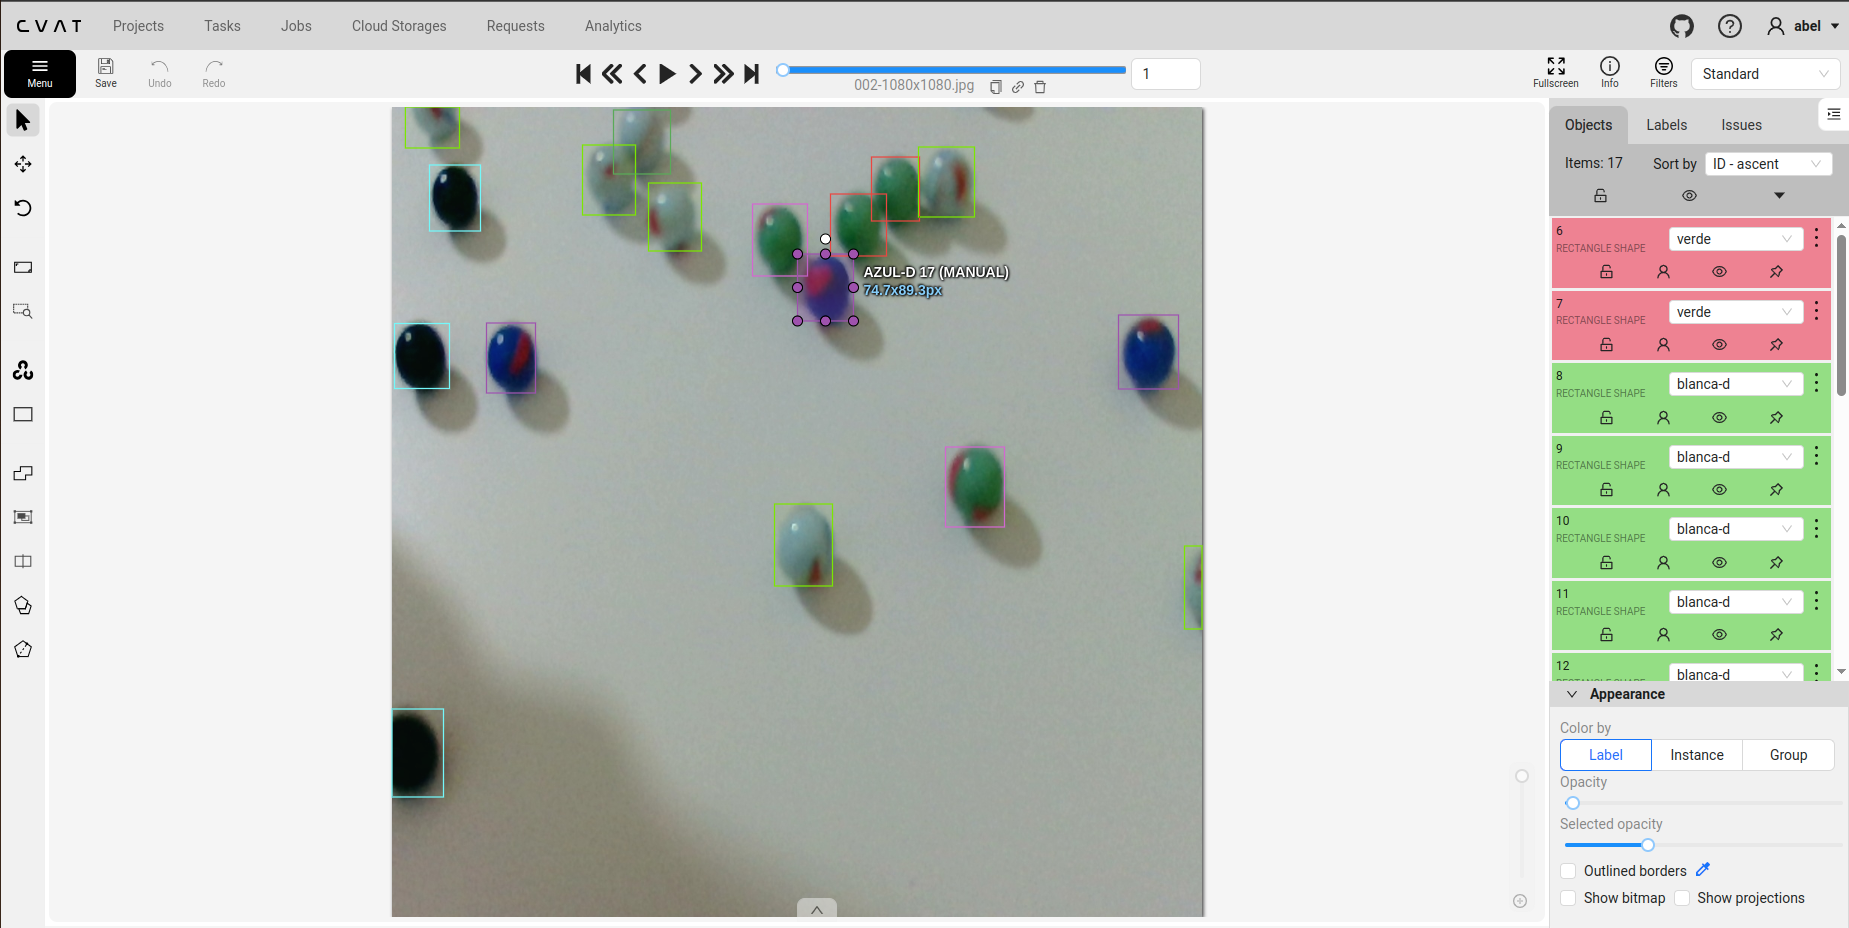
\includegraphics[width=0.8\textwidth]{images/diseno_e_implementacion/ejemplo_CVAT.png}
   \caption{Ejemplo de anotación de imágenes utilizando CVAT.}
   \label{fig:cvat_anotacion}
\end{figure}


Este formato sigue una estructura de texto simple, donde cada línea representa una anotación para un objeto en la imagen. Cada línea contiene cinco valores: el índice de la clase (0 para canica blanca, 1 para canica negra, 2 para canica azul, 3 para canica verde, 4 para canica blanca con defecto, 5 para canica negra con defecto, 6 para canica azul con defecto y 7 para canica verde con defecto), seguido de las coordenadas normalizadas del centro de la caja delimitadora (x, y) y su ancho y alto (w, h), todos ellos en relación a las dimensiones de la imagen.

Volviendo al dataset, se capturaron un total de 600 imágenes, de las cuales el 80\% se utilizaron para el entrenamiento, el 10\% para la validación y el 10\% restante para el testeo del modelo. Esta división es crucial para garantizar que el modelo no solo aprenda a detectar los objetos en las imágenes de entrenamiento, sino que también generalice bien a nuevas imágenes que no ha visto antes. La validación se utiliza para ajustar los hiperparámetros del modelo y evitar el sobreajuste (overfitting), mientras que el conjunto de testeo proporciona una evaluación final del rendimiento del modelo.


Como se ha mencionado en la sección \ref{sec:one_stage_detectors} y se detalla en la Tabla \ref{tab:yolo_all_variants_comparison}, los modelos YOLO presentan diversas variantes que difieren en tamaño, complejidad, latencia y precisión. Esta tabla comparativa es fundamental para seleccionar el modelo que mejor equilibre la velocidad de procesamiento y la precisión requerida.

Para este trabajo, se han entrenado y evaluado experimentalmente las siguientes variantes: YOLOv5n, YOLOv5m, YOLOv8n, YOLOv8s, YOLO11n, YOLO11s, YOLO11m y YOLO11l.




\begin{table}[H]
   \centering
   \resizebox{\textwidth}{!}{%
   \begin{tabular}{llc|c|ccl} % Familia (l), Variante (l), Tamaño (c) | Parámetros (M) (c) | Lat CPU (c), Lat GPU (c), GPU Tipo (l)
      \toprule
      Familia & Variante & Tamaño (px) & Parámetros (M) & Latencia CPU ONNX (ms) & Latencia GPU (ms) & GPU (para Latencia) \\
      \midrule
      \multirow{2}{*}{YOLOv5} & nu & 640 & 2.6 & 73.6 & 1.06 & \multirow{2}{*}{A100 TensorRT} \\
       & mu & 640 & 25.1 & 233.9 & 1.86 & \\
      \midrule
      \multirow{2}{*}{YOLOv8} & n & 640 & 3.2 & 80.4 & 0.99 & \multirow{2}{*}{A100 TensorRT} \\
       & s & 640 & 11.2 & 128.4 & 1.20 & \\
      \midrule
      \multirow{5}{*}{YOLO11} & n & 640 & 2.6 & 56.1 ± 0.8 & 1.5 ± 0.0 & \multirow{5}{*}{T4 TRT10} \\
       & s & 640 & 9.4 & 90.0 ± 1.2 & 2.5 ± 0.0 & \\
       & m & 640 & 20.1 & 183.2 ± 2.0 & 4.7 ± 0.1 & \\
       & l & 640 & 25.3 & 238.6 ± 1.4 & 6.2 ± 0.1 & \\
       & x & 640 & 56.9 & 462.8 ± 6.7 & 11.3 ± 0.2 & \\
      \bottomrule
   \end{tabular}
   }
   \caption{Análisis comparativo de variantes de YOLO (v5, v8, v11) indicando tamaño, parámetros, latencias CPU/GPU y la GPU específica utilizada para la medición de latencia GPU.}
   \label{tab:yolo_all_variants_comparison}
\end{table}


Para el entrenamiento de los modelos se han seleccionado los siguientes hiperparámetros:
\begin{itemize}
   \item \textbf{Tasa de aprendizaje (learning rate):} Se ha utilizado un valor inicial de 0.01, con un ajuste posterior basado en la tasa de convergencia observada durante el entrenamiento.
   \item \textbf{Número de épocas (epochs):} Se han realizado 30 épocas, para permitir que el modelo aprenda de manera efectiva sin caer en el sobreajuste.
   \item \textbf{Tamaño del lote (batch size):} Se ha establecido en 16, lo que permite un equilibrio entre la velocidad de entrenamiento y la utilización de memoria.
   \item \textbf{Tamaño de imagen (image size):} Se ha utilizado una resolución de 640x640 píxeles, que es un tamaño estándar para los modelos YOLO y proporciona un buen compromiso entre precisión y velocidad.
   \item \textbf{Optimizador:} Se ha utilizado el optimizador AdamW, que es conocido por su eficacia en el entrenamiento de modelos de aprendizaje profundo.
   \item \textbf{Tasa de aumento de datos (data augmentation):} Se han aplicado técnicas de aumento de datos como rotación, cambio de brillo y contraste, y recortes aleatorios para mejorar la generalización del modelo.
   \item \textbf{Device:} Se ha utilizado una Jetson AGX Xavier, que proporciona un entorno de hardware optimizado para el entrenamiento.
\end{itemize}



Los resultados del entrenamiento se han evaluado utilizando el conjunto de validación, y se han registrado métricas como la precisión (precision), la recuperación (recall) y el mAP (mean Average Precision). Estas métricas son fundamentales para entender el rendimiento del modelo y su capacidad para generalizar a nuevos datos.

\begin{table}[H]
   \centering
   \begin{tabular}{l | c | c | c | c | c}
      \toprule
      Modelo & Tiempo (h) & Precisión & Recall & mAP50 & mAP50-95 \\
      \midrule
      YOLOv5nu & 0.128 & 0.898 & 0.922 & 0.939 & 0.759 \\
      YOLOv5mu & 0.333 & 0.952 &  0.928 & 0.955 & 0.790 \\
      YOLOv8n & 0.137 & 0.934 & 0.905 & 0.950 & 0.770 \\
      YOLOv8s & 0.202 & 0.943 & 0.928 & 0.955 & 0.786 \\
      YOLO11n & 0.140 & 0.950 & 0.882 & 0.939 & 0.761 \\
      YOLO11s & 0.192 & 0.941 & 0.936 & 0.963 & 0.796 \\
      YOLO11m & 0.377 & 0.941 & 0.936 & 0.963 & 0.796 \\
      YOLO11l & 0.485 & 0.954 & 0.947 & 0.967 & 0.801 \\
      \bottomrule
   \end{tabular}
   \caption{Comparativa del rendimiento de los modelos YOLOv5, YOLOv8 y YOLO11 en términos de tiempo de entrenamiento, precisión, recall y mAP.}
   \label{tab:modelos_metrics}
\end{table}

La Tabla \ref{tab:modelos_metrics} resume los resultados del entrenamiento para las variantes de YOLOv5, YOLOv8 y YOLO11. Se observa una tendencia general: a medida que aumenta la complejidad del modelo (de las versiones más pequeñas a las más grandes dentro de cada familia), tanto la precisión como el recall experimentan una mejora constante. Esto sugiere que los modelos de mayor tamaño poseen una capacidad superior para aprender representaciones de características más ricas y discriminativas, resultando en una detección de objetos más efectiva. No obstante, esta mejora en el rendimiento se acompaña de un incremento en el tiempo de entrenamiento y la demanda de recursos computacionales, lo que refleja el inherente compromiso entre la capacidad del modelo y la eficiencia del proceso de aprendizaje.

\begin{figure}[H]
   \centering
   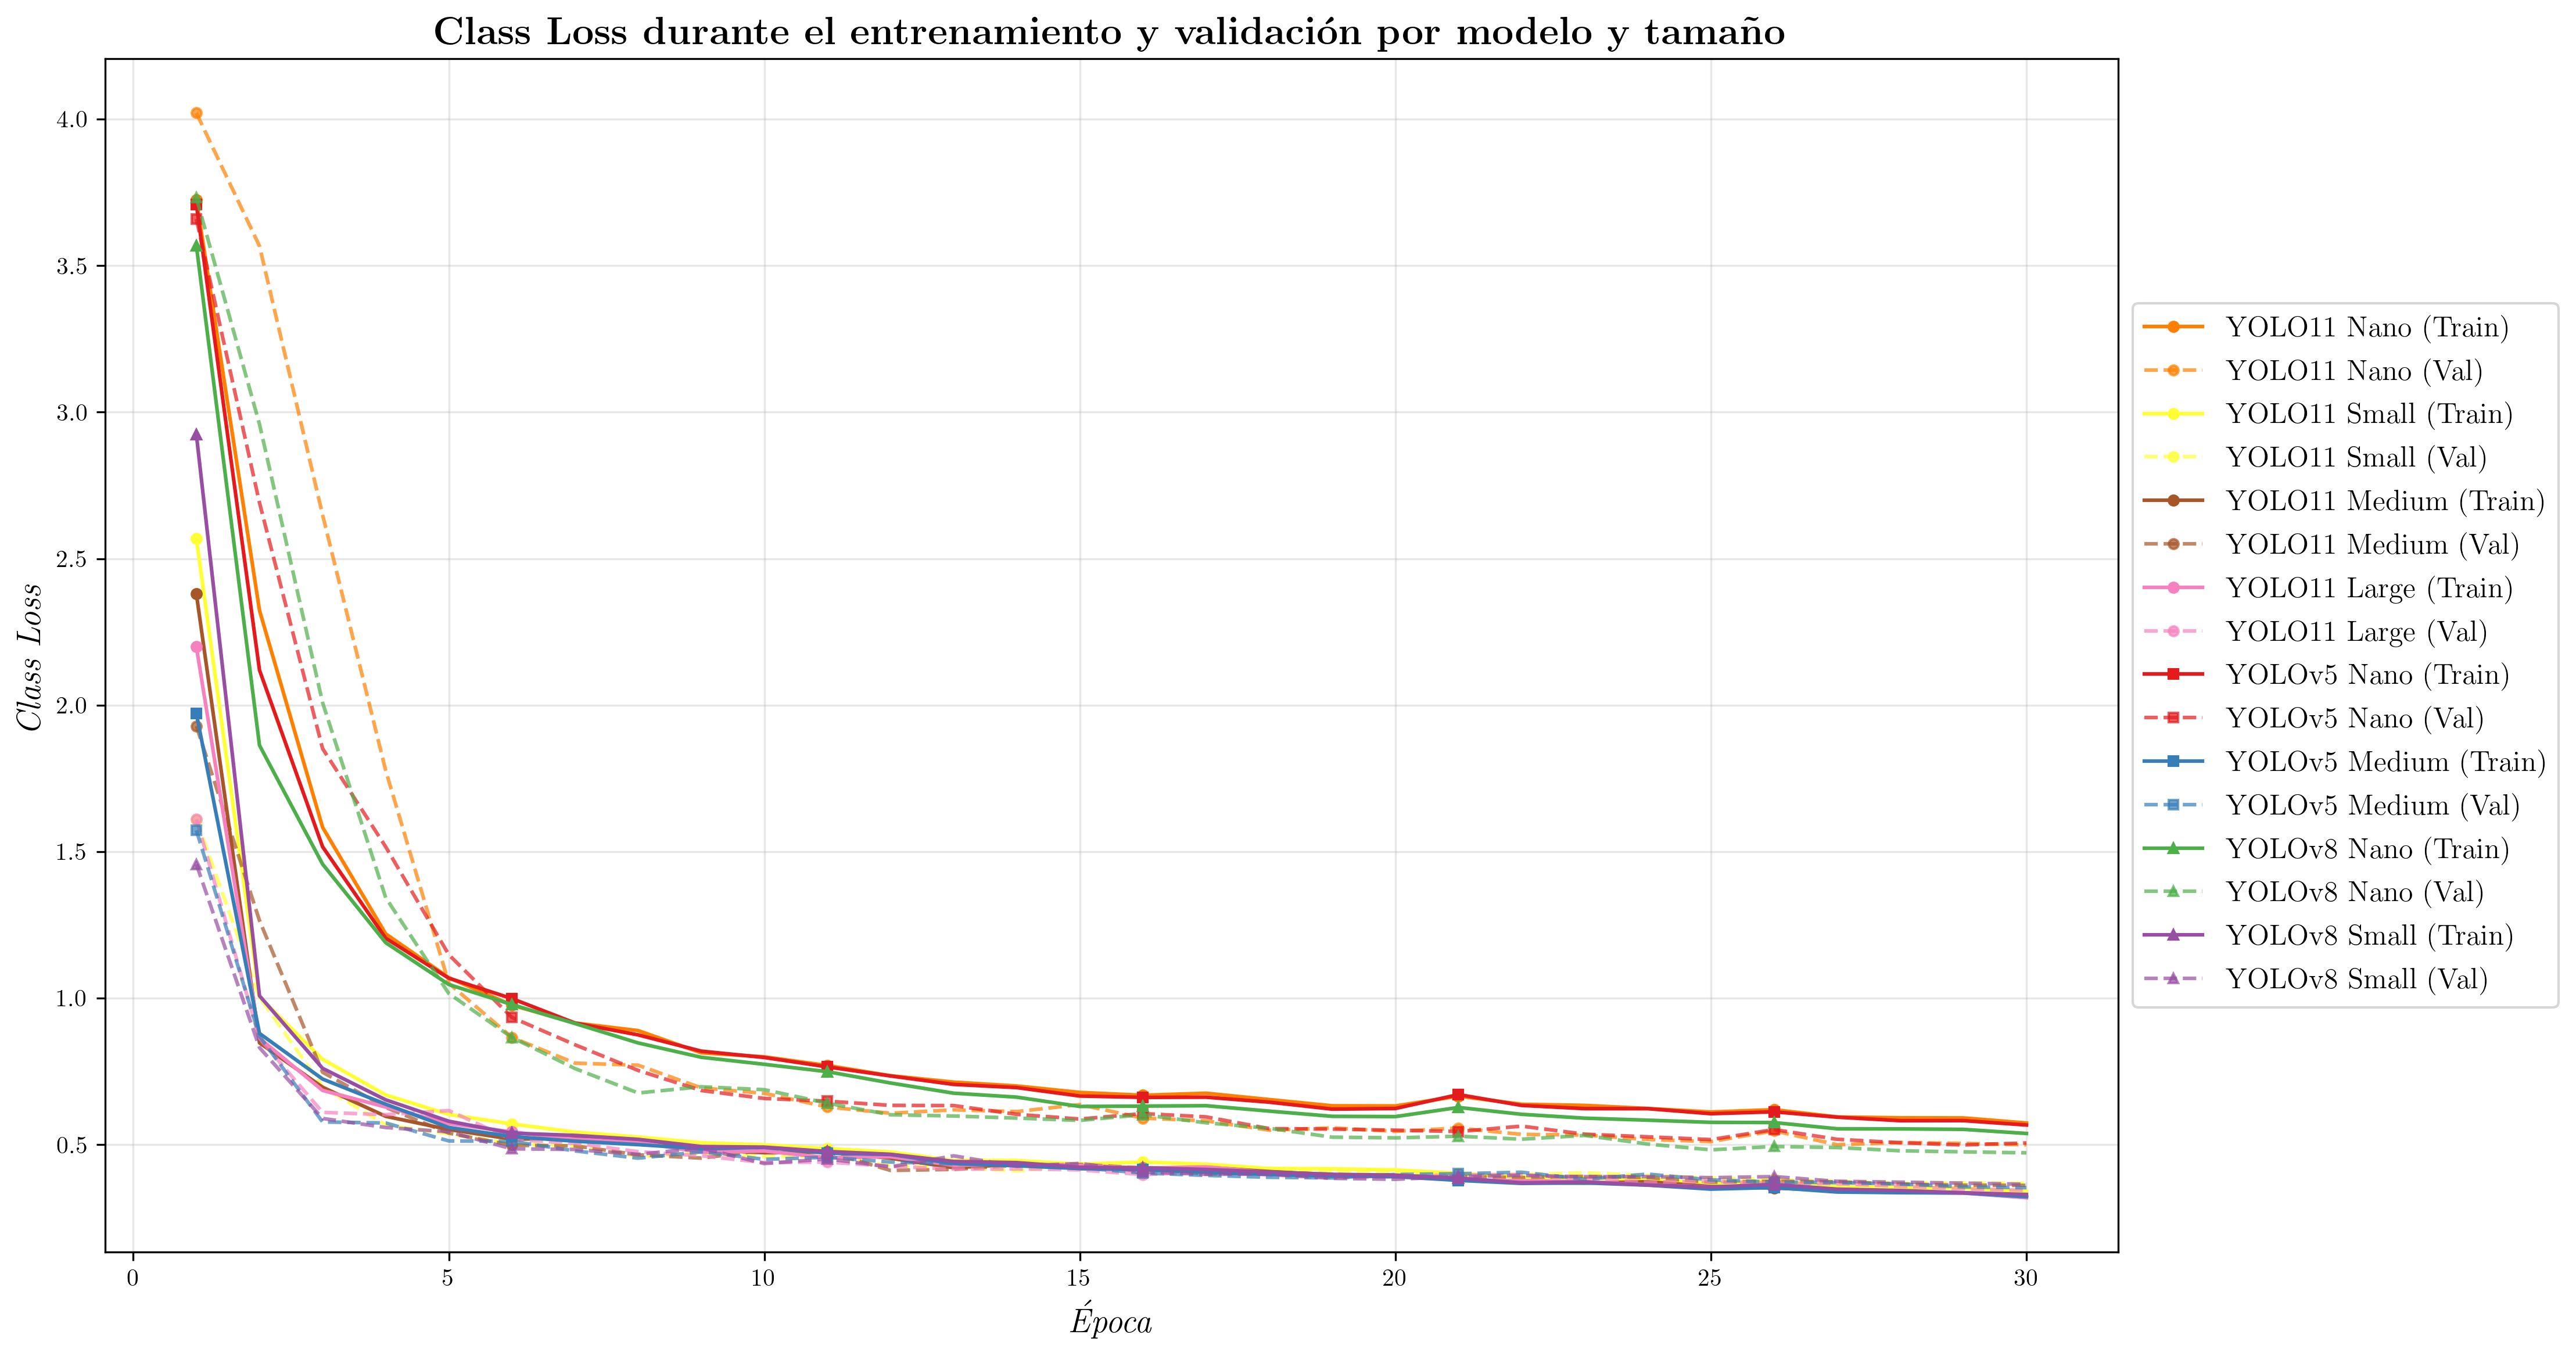
\includegraphics[width=0.8\textwidth]{excels/entrenamiento/loss_plot.png}
   \caption{Curvas de pérdida de entrenamiento y validación para las distintas tallas de modelos YOLOv5, YOLOv8 y YOLO11.}
   \label{fig:loss_curves}
\end{figure}

La Figura \ref{fig:loss_curves} presenta las curvas de pérdida (loss) durante el entrenamiento y la validación para las diferentes variantes de YOLOv5, YOLOv8 y YOLOv11. Estas gráficas evidencian una progresiva disminución de la función de pérdida a lo largo de las épocas, lo cual es un indicador clave de que cada modelo está aprendiendo a generalizar a partir de los datos para la tarea de detección de objetos. Es notable que, en todas las familias, la pérdida de validación sigue una tendencia descendente similar a la de entrenamiento, sugiriendo una buena capacidad de generalización y la ausencia de un sobreajuste significativo. Se aprecia un descenso pronunciado de la pérdida en las épocas iniciales, indicativo de una rápida asimilación de patrones, y conforme avanza el entrenamiento, la tasa de reducción disminuye gradualmente hasta alcanzar una meseta. Este comportamiento es característico en el entrenamiento de modelos de aprendizaje profundo y señala la convergencia hacia un mínimo local en la función de pérdida, donde las mejoras adicionales resultan marginales.



\section{Descripción del sistema} \label{sec:descripcion_sistema}

El sistema está organizado como una serie de etapas de procesamiento secuenciales que trabajan de forma coordinada para lograr la detección y seguimiento de objetos en tiempo real. Como se muestra en la Figura~\ref{fig:sistema_propuesto}, el sistema recibe como entrada imágenes de una cámara y consta de cuatro componentes principales: un módulo de captura de imágenes que obtiene los fotogramas del vídeo, un módulo de inferencia que ejecuta el modelo de detección de objetos, un módulo de seguimiento que implementa el algoritmo BYTETrack para mantener la identidad de los objetos detectados, y un módulo de escritura que gestiona la salida del sistema.
\begin{figure}[H]
   \centering
   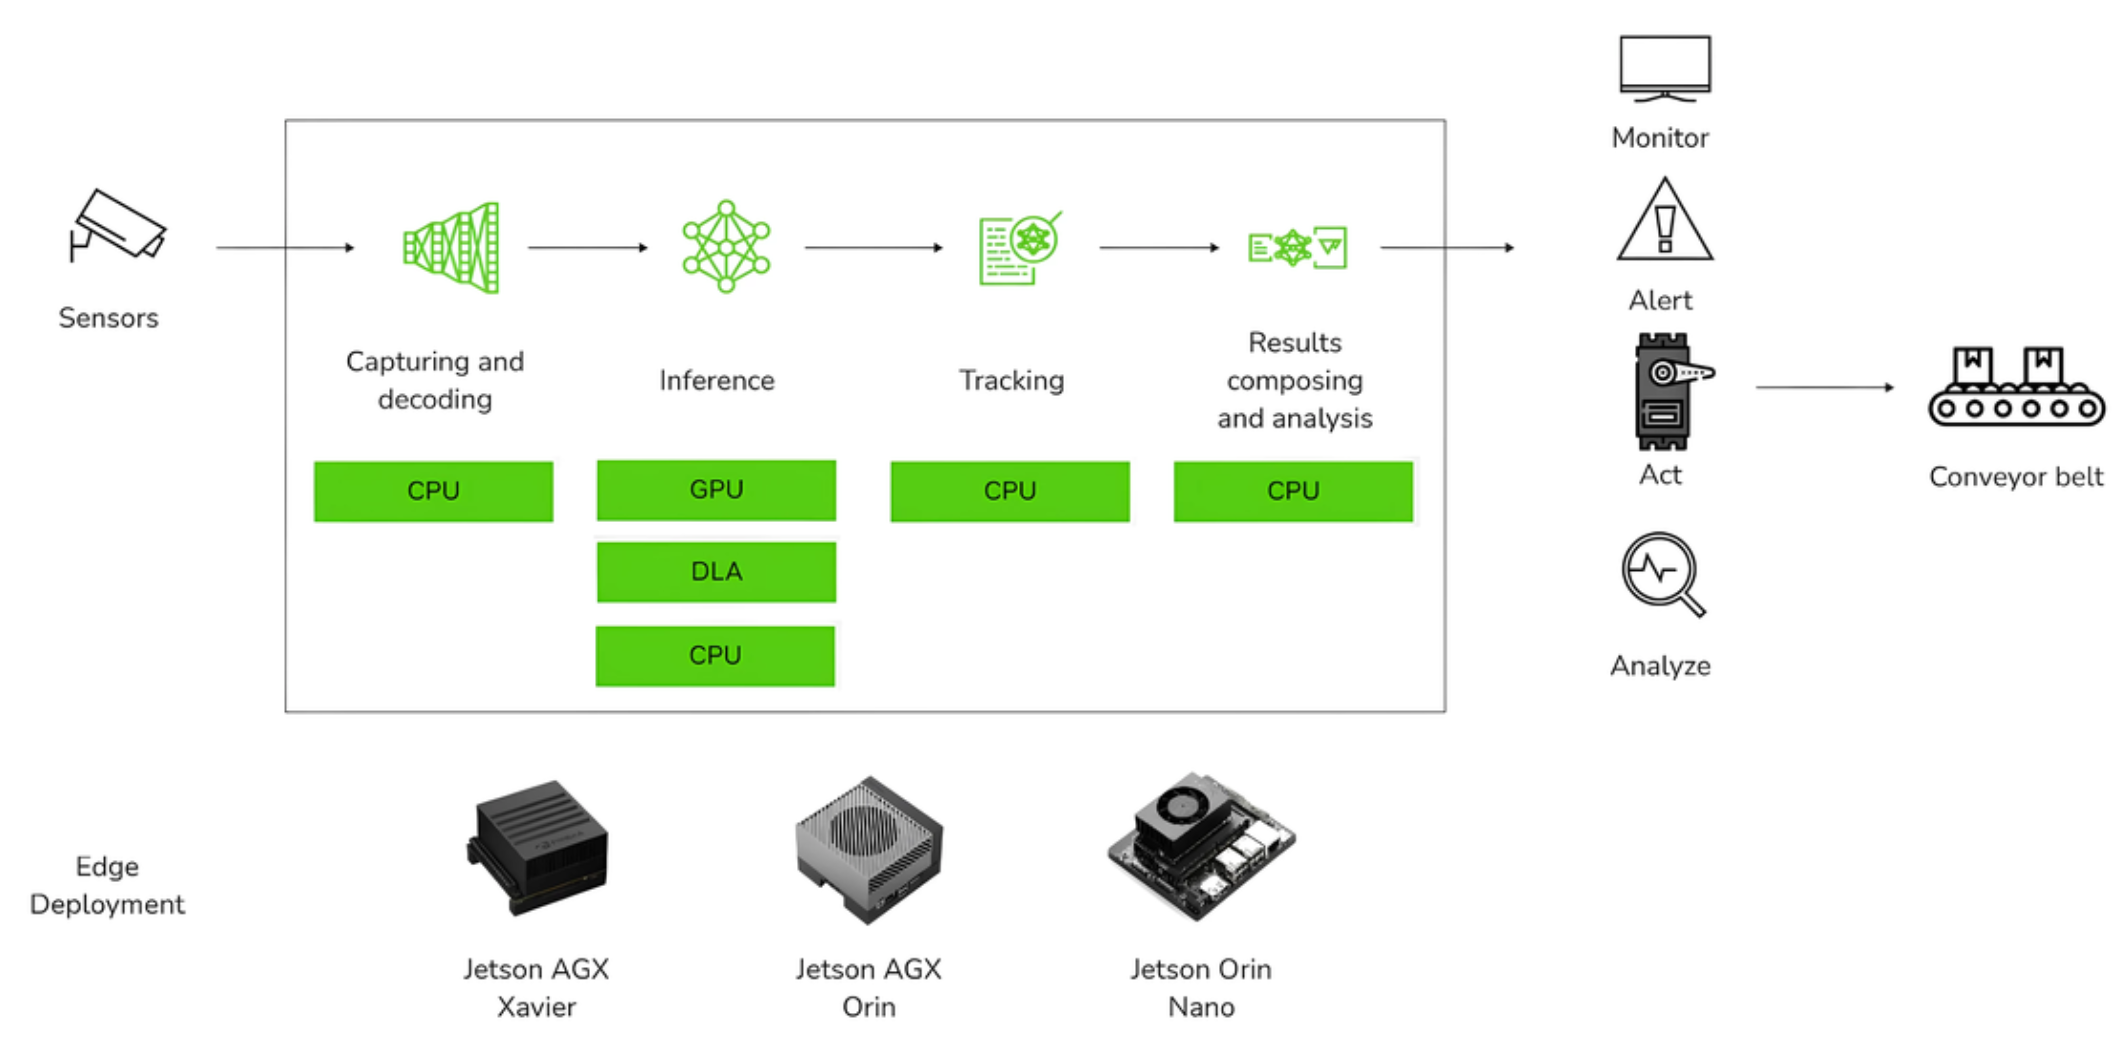
\includegraphics[width=0.95\textwidth]{images/diseno_e_implementacion/figura_TFG_v3.png}
   \caption{Figura del sistema propuesto.}
   \label{fig:sistema_propuesto}
\end{figure}

Los resultados del sistema pueden utilizarse de diversas formas, monitorización en tiempo real a través de visualización de las detecciones, generación de alertas basadas en reglas predefinidas, interacción con sistemas de control automatizado para realizar acciones específicas, y almacenamiento de datos para su posterior análisis y extracción de métricas que permitan optimizar procesos industriales.

La arquitectura del sistema se ha diseñado estratégicamente para maximizar el rendimiento computacional y la eficiencia en el uso de recursos, asegurando una operación coordinada entre sus componentes modulares. Los datos fluyen secuencialmente a través de las distintas etapas, permitiendo un procesamiento continuo y eficaz de la información visual. Esta estructura modular intrínseca no solo simplifica el mantenimiento y las futuras actualizaciones, sino que también dota al sistema de una gran flexibilidad para adaptarse a diferentes requisitos operativos y escenarios de despliegue. Aunque optimizado específicamente para la plataforma NVIDIA Jetson, su diseño modular facilita su potencial portabilidad a otras plataformas hardware de NVIDIA, como GPUs de escritorio o servidores de alto rendimiento, siempre que se cumplan los prerrequisitos de hardware y software.


\section{Diseño de las etapas del sistema} \label{sec:diseno_etapas}
 
El sistema propuesto se compone de cuatro etapas principales, cada una de las cuales desempeña un papel crucial en el procesamiento y análisis de las imágenes capturadas. A continuación, se describen en detalle cada una de estas etapas.

\subsection{Captura de imágenes} \label{sec:captura_imagenes}

La etapa de captura de imágenes es la responsable de adquirir los fotogramas del flujo de vídeo en tiempo real. Sus funciones abarcan la configuración y el control de la cámara, la adquisición de las imágenes y su posible preprocesamiento inicial antes de ser transferidas al módulo de inferencia. Para la implementación de este módulo se ha empleado la biblioteca OpenCV, la cual ofrece una interfaz robusta y eficiente para la interacción con dispositivos de captura y el procesamiento básico de imágenes. La cámara se configura para operar a una resolución y tasa de fotogramas adecuadas a los requisitos de la aplicación. El preprocesamiento puede incluir diversas operaciones, tales como la conversión a escala de grises, la normalización de píxeles o el redimensionamiento, adaptándose a las especificaciones del modelo de detección de objetos utilizado. En el sistema desarrollado, se empleó una cámara de alta definición capaz de alcanzar una resolución máxima de 1920x1080 píxeles y una tasa de 30 fps. Si bien se experimentó con diversas configuraciones de resolución y tasa de fotogramas según las necesidades de cada prueba, la configuración estándar para la mayoría de los experimentos fue de 640x640 píxeles a 30 fps. Esta etapa se ejecuta íntegramente en la CPU.

\subsection{Inferencia} \label{sec:inferencia}
La etapa de inferencia constituye el núcleo computacional del sistema, siendo responsable de ejecutar el modelo de detección de objetos preentrenado sobre cada fotograma adquirido por la etapa de captura. Para esta tarea crucial, se ha seleccionado el modelo \gls{yolo}11, una variante optimizada dentro de la familia \gls{yolo}, reconocida por su equilibrio entre velocidad y precisión en tareas de detección en tiempo real. La implementación se apoya en el framework de Ultralytics \cite{Jocher_Ultralytics_YOLO_2023}, una biblioteca de alto nivel que simplifica significativamente el ciclo de vida de los modelos YOLO, desde el entrenamiento hasta el despliegue y la inferencia, ofreciendo una interfaz robusta y eficiente.

El proceso de inferencia comienza con la adquisición de un fotograma de vídeo, que se convierte en un tensor adecuado para la entrada del modelo. Este tensor es una representación numérica de la imagen, donde cada píxel se traduce en un valor que el modelo puede procesar. La transformación del fotograma a tensor incluye operaciones como la normalización y el redimensionamiento, asegurando que los datos estén en el formato correcto para el modelo YOLO11.
La ejecución de la inferencia propiamente dicha implica cargar el modelo \gls{yolo}11 (potencialmente optimizado mediante NVIDIA TensorRT para maximizar el rendimiento en la plataforma Jetson) y pasarle el tensor de entrada. Aprovechando la aceleración por hardware (\gls{gpu} y/o \gls{dla}s disponibles en los módulos Jetson), el modelo procesa la imagen y genera un conjunto de predicciones. Estas predicciones iniciales suelen ser numerosas y requieren un postprocesamiento para refinar los resultados. Este postprocesamiento, a menudo gestionado internamente por el framework Ultralytics o aplicado explícitamente, incluye la aplicación de un umbral de confianza para descartar detecciones poco fiables y la ejecución del algoritmo de \gls{nms} para eliminar cajas delimitadoras redundantes que correspondan al mismo objeto.

El resultado final de la etapa de inferencia, que se transfiere a la etapa de seguimiento, es una lista estructurada de las detecciones finales para el fotograma actual. Cada detección en esta lista contiene información esencial: las coordenadas de la caja delimitadora que localiza al objeto (comúnmente en formato (x, y, w, h), donde (x, y) representan las coordenadas del centro de la caja, y (w, h) su anchura y altura), una puntuación de confianza que cuantifica la fiabilidad de la detección, y la etiqueta de la clase predicha para el objeto (p. ej., 'canica\_azul', 'canica\_verde\_defecto'). La eficiencia y rapidez de esta etapa son críticas para mantener la capacidad de procesamiento en tiempo real del sistema global.

\subsection{Seguimiento} \label{sec:seguimiento}
La etapa de seguimiento es la encargada de mantener la identidad de los objetos detectados a lo largo del tiempo, asegurando que cada objeto en el flujo de vídeo conserve su etiqueta y trayectoria a pesar de las variaciones en su posición, apariencia o posibles oclusiones. Para lograr esto, se ha utilizado la implementación del algoritmo BYTETrack en el framework de Ultralytics\cite{Jocher_Ultralytics_YOLO_2023}, que se basa en un enfoque de seguimiento por detección explicado en la subsección~\ref{sec:bytetrack}. Este algoritmo se encarga de asociar las detecciones generadas por la etapa de inferencia con las trayectorias existentes, utilizando tanto las detecciones de alta confianza como las de baja confianza para mejorar la robustez del seguimiento.

Para la configuración del algoritmo BYTETrack existen varios parámetros ajustables que permiten optimizar su rendimiento según las características específicas del entorno y los objetos a seguir. Estos parámetros son:
\begin{itemize}
   \item \texttt{track\_high\_thresh}: Umbral de confianza para considerar una detección como de alta confianza (valor típico: 0.6). Las detecciones por encima de este umbral se utilizan en la primera etapa de asociación.
   \item \texttt{track\_low\_thresh}: Umbral de confianza para considerar una detección como de baja confianza (valor típico: 0.15). Las detecciones que se encuentren entre este umbral y \texttt{track\_high\_thresh} se utilizan en la segunda etapa de asociación para recuperar objetos ocluidos.
   \item \texttt{new\_track\_thresh}: Umbral de confianza mínimo para iniciar una nueva trayectoria a partir de una detección de alta confianza no asociada (valor típico: 0.6). Debe ser al menos tan alto como \texttt{track\_high\_thresh}.
   \item track\_buffer: Número máximo de fotogramas que una trayectoria puede permanecer sin asociar antes de ser eliminada. Define la ``edad'' máxima de una pista perdida. Un valor típico es 30 fotogramas.
   \item \texttt{match\_thresh}: Umbral de IoU (Intersection over Union) para la asociación entre las predicciones del Filtro de Kalman y las detecciones (valor típico: 0.8). Si la IoU es mayor que este umbral, se considera una coincidencia potencial.
\end{itemize}

Este algoritmo se basa en un ciclo continuo de predicción y corrección, donde el Filtro de Kalman se utiliza para predecir la posición futura de los objetos y suavizar las trayectorias, manejando la incertidumbre en las mediciones. La asociación de detecciones y trayectorias se realiza mediante un algoritmo de asignación, como el algoritmo Húngaro, que busca minimizar el costo total de la asociación entre las detecciones y las trayectorias existentes. Se ejecuta íntegramente en la CPU debido a la implementación del algoritmo en la biblioteca de Ultralytics.

Tras aplicar la asociación de detecciones y trayectorias, el algoritmo ofrece como salida una lista con el identificador único de cada objeto, su clase, la puntuación de confianza y las coordenadas de la caja delimitadora. Esta información es fundamental para la siguiente etapa del sistema.

\subsection{Escritura de resultados} \label{sec:escritura_resultados}

La etapa de escritura de resultados es responsable de gestionar la salida del sistema, que puede adoptar diversas formas según los requisitos específicos de la aplicación. Esta etapa se encarga de presentar los resultados de manera comprensible y útil, permitiendo su interpretación y análisis posterior. Las principales funciones de esta etapa incluyen la visualización de los resultados en tiempo real, la generación de alertas basadas en reglas predefinidas y el almacenamiento de datos para su posterior análisis. También se encarga de los posibles conexiones a sistemas de control automatizado, permitiendo la interacción con otros sistemas o dispositivos.

\begin{figure}[H]
   \centering
   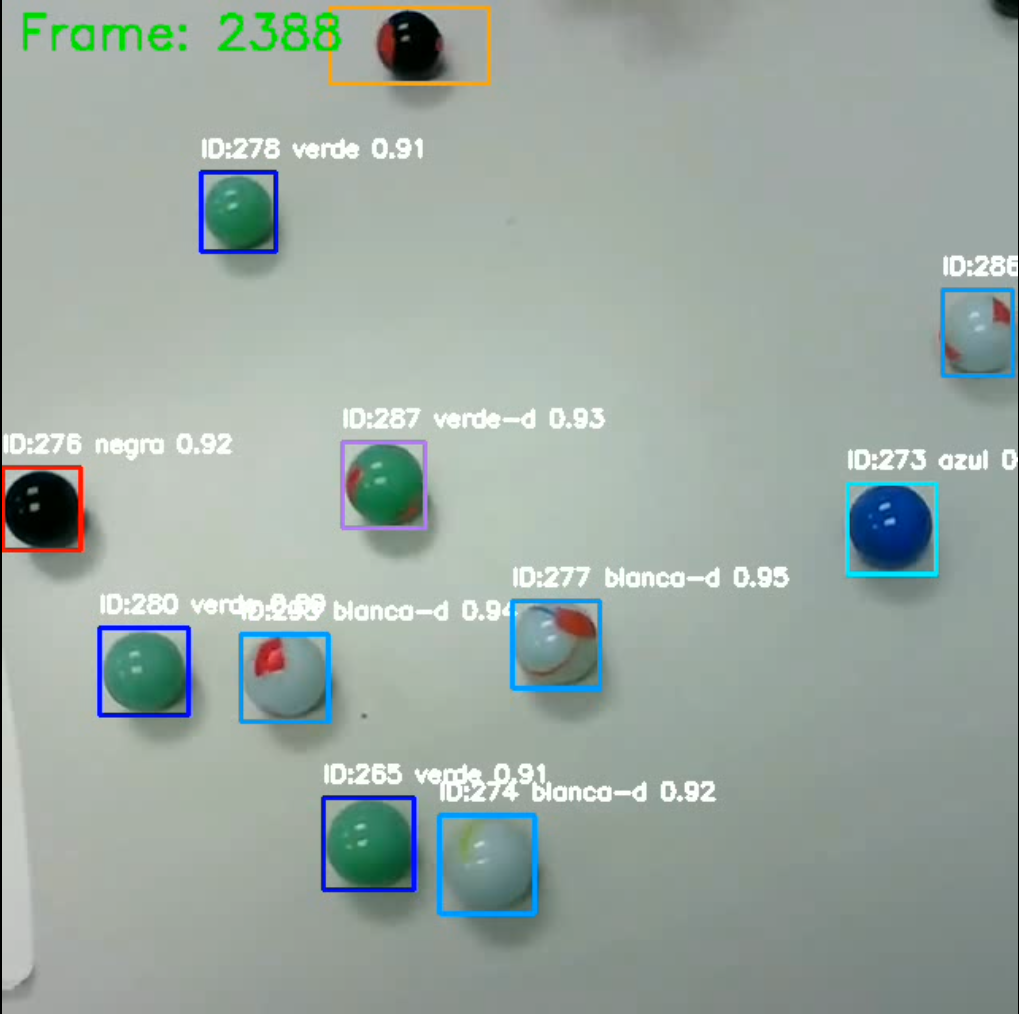
\includegraphics[width=0.5\textwidth]{images/diseno_e_implementacion/ejemplo_canicas_resultado.png}
   \caption{Ejemplo de salida del sistema.}
   \label{fig:resultado_sistema}
\end{figure}

La Figura \ref{fig:resultado_sistema} muestra un ejemplo de la salida del sistema, donde se visualizan las detecciones y trayectorias de los objetos en el flujo de vídeo. Cada objeto detectado está representado por una caja delimitadora que incluye su etiqueta de clase y un identificador único. Esta representación gráfica permite una rápida identificación y seguimiento de los objetos en movimiento, facilitando la monitorización en tiempo real del sistema.

\section{Segmentación de las etapas del sistema} \label{sec:segmentacion_etapas}

Tras la implementación de las etapas del sistema, se ha considerado la posibilidad de segmentar el sistema mediante estas etapas para mejorar el rendimiento y la eficiencia del procesamiento. La segmentación permite distribuir la carga de trabajo entre diferentes unidades de procesamiento, optimizando así el uso de los recursos disponibles en la plataforma.

La segmentación de las etapas del sistema se puede realizar de varias maneras, dependiendo de los requisitos específicos de la aplicación y de los recursos disponibles. A continuación, se describen las diferentes opciones de segmentación que se han consideradom, implementado y evaluado en el sistema propuesto.
    
\subsection{Secuencial} \label{sub:secuencial}

La primera y mas trivial opción es la ejecución secuencial de las etapas del sistema. En este enfoque, cada etapa se ejecuta de forma consecutiva, donde la salida de una etapa se convierte en la entrada de la siguiente. Este método es el más sencillo de implementar y no requiere una configuración adicional para la comunicación entre etapas. Sin embargo, presenta limitaciones significativas en términos de rendimiento y eficiencia, ya que no aprovecha al máximo los recursos disponibles. Si se hace la analogía con un procesador, este enfoque se asemeja a un procesador no segmentado.

\begin{figure}[H]
   \centering
   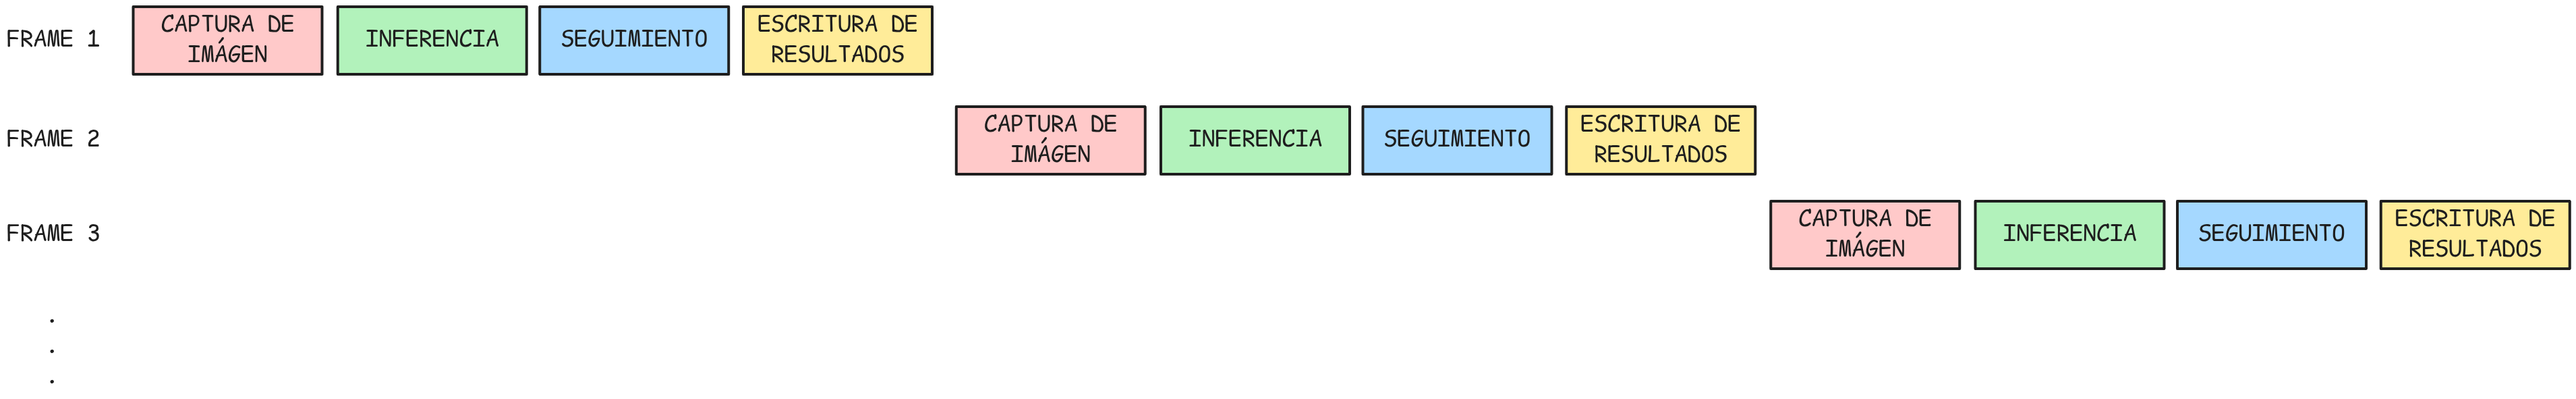
\includegraphics[width=1\textwidth]{images/diseno_e_implementacion/secuencial.png}
   \caption{Diagrama de flujo del sistema sin segmentar.}
   \label{fig:secuencial}
\end{figure}

La Figura \ref{fig:secuencial} ilustra el flujo de datos en un sistema secuencial. En este diagrama, cada etapa del sistema se ejecuta de forma lineal, donde la salida de una etapa se convierte en la entrada de la siguiente. Este enfoque es fácil de entender y de implementar, pero no aprovecha al máximo los recursos disponibles.

\subsection{Segmentación basada en hilos} \label{sub:segmentacion_hilos}

La segunda opción es la segmentación del sistema en diferentes hilos. En este enfoque, cada etapa principal del sistema (captura, inferencia, seguimiento, escritura) se ejecuta en un hilo (\textit{thread}) independiente. A diferencia del enfoque secuencial donde cada etapa debe esperar a que la anterior finalice, la segmentación por hilos permite que las etapas operen de forma concurrente, solapando sus ejecuciones. Esto puede mejorar significativamente el rendimiento (throughput) y reducir la latencia, ya que mientras una etapa espera por una operación (p. ej., E/S de la cámara), otra etapa puede estar procesando datos (p. ej., inferencia en GPU o seguimiento en CPU). Los hilos operan dentro del mismo proceso, compartiendo el mismo espacio de memoria. La comunicación y transferencia de datos (fotogramas, detecciones) entre estas etapas/hilos se gestiona mediante colas de mensajes (\textit{Queue}) de la librería estándar de Python, que aseguran una transferencia eficiente y segura entre hilos (\textit{thread-safe}).


En Python, un hilo es una unidad básica de ejecución. Sin embargo, al trabajar con hilos en Python, es crucial entender el impacto del \gls{gil} (Global Interpreter Lock). El \gls{gil} es un mecanismo de bloqueo mutuo (mutex) que protege el acceso al intérprete de Python. Su función principal es permitir que solo un hilo ejecute código de bytes Python (\textit{Python bytecode}) a la vez dentro de un único proceso, incluso si el sistema dispone de múltiples núcleos de CPU. Es decir, en Python, debido al \gls{gil}, dos hilos de un mismo proceso no pueden ejecutar código Python de manera simultánea en núcleos de CPU diferentes. Esta restricción se implementó originalmente para simplificar la gestión de memoria (específicamente, el conteo de referencias) y prevenir condiciones de carrera en el acceso a objetos Python.

La principal consecuencia del \gls{gil} es que impide el verdadero paralelismo para tareas que son intensivas en \gls{cpu} (\textit{CPU-bound}) y están escritas puramente en Python. Aunque se creen múltiples hilos, solo uno podrá ejecutar código Python en un instante dado. En aplicaciones con muchos hilos compitiendo por la \gls{cpu}, el \gls{gil} puede incluso introducir sobrecarga y contención, llevando a un rendimiento inferior al de una ejecución secuencial.

No obstante, el \gls{gil} no bloquea la ejecución en todas las circunstancias. Se libera automáticamente durante operaciones que no ejecutan código Python directamente, como:
\begin{itemize}
   \item Operaciones de entrada/salida (E/S): Lectura/escritura de archivos, operaciones de red, interacción con dispositivos como cámaras.
   \item Llamadas a código nativo compilado: Cuando se utilizan bibliotecas como NumPy, SciPy, o las bibliotecas específicas para la ejecución en GPU (como las de CUDA/TensorRT), que realizan el cómputo fuera del intérprete Python.
   \item Llamadas explícitas de espera: Como `time.sleep()`.
\end{itemize}


\begin{figure}[H]
   \centering
   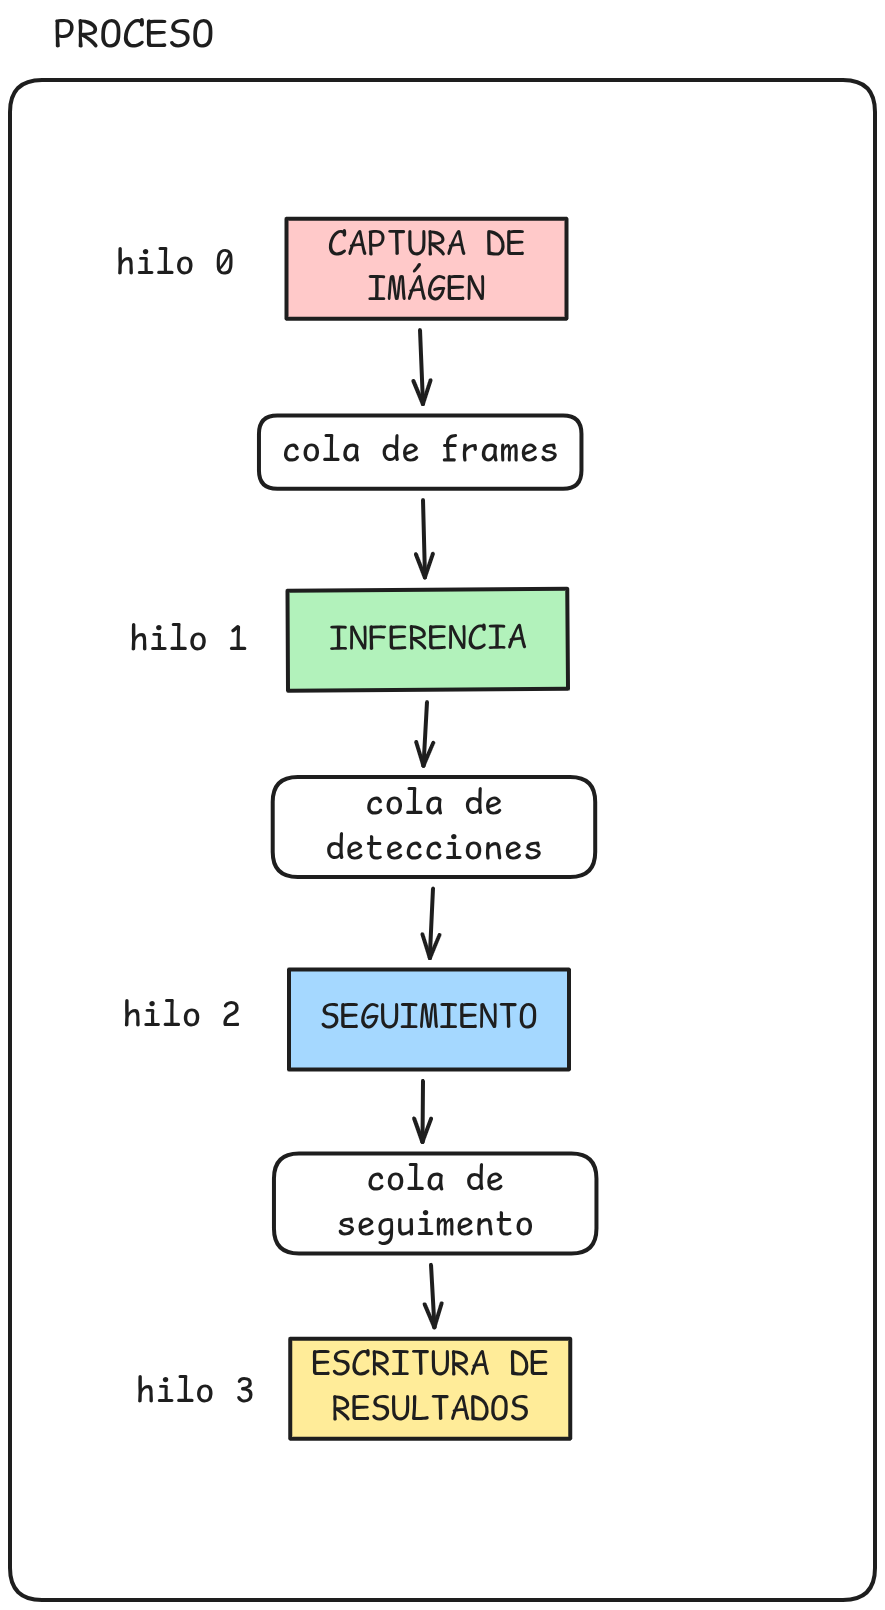
\includegraphics[width=0.3\textwidth]{images/diseno_e_implementacion/segmentacion_hilos.png}
   \caption{Diagrama de flujo del sistema segmentado en hilos.}
   \label{fig:hilos}

\end{figure}

La Figura~\ref{fig:hilos} ilustra este enfoque, donde cada etapa opera en su propio hilo y se comunica mediante colas.

Considerando estas características, la segmentación basada en hilos puede ser beneficiosa para nuestro sistema. La etapa de captura de imágenes es intensiva en E/S. La etapa de inferencia, especialmente cuando se ejecuta en la GPU o DLA utilizando bibliotecas optimizadas como TensorRT, realiza la mayor parte de su trabajo en código nativo, liberando el \gls{gil}. La etapa de escritura también implica operaciones de E/S. Durante los momentos en que estas etapas liberan el \gls{gil}, otros hilos pueden progresar.

Aunque más complejo de implementar que el enfoque secuencial debido a la necesidad de sincronización y comunicación entre hilos, este modelo permite una mejor utilización de los recursos y mejora la capacidad de respuesta y el rendimiento general del sistema al solapar operaciones de E/S y cómputo intensivo (en GPU/DLA) con otras tareas.

\subsection{Segmentación basada en procesos} \label{sub:segmentacion_procesos}

La tercera opción es la segmentación del sistema en diferentes procesos. En este enfoque, cada etapa principal del sistema (captura, inferencia, seguimiento, escritura) se ejecuta en un proceso independiente. La comunicación y transferencia de datos entre estas etapas/procesos se gestiona mediante colas de mensajes (\textit{Queue}). Estas colas provienen del módulo `multiprocessing` de la librería estándar de Python y comparten la misma interfaz que las colas estándar del módulo `queue`, lo que asegura una transferencia eficiente y segura entre procesos (\textit{process-safe}).

La principal ventaja de este enfoque es que cada etapa del sistema se ejecuta en su propio proceso independiente, lo que permite un mejor aprovechamiento de los recursos disponibles. Además, al estar cada etapa en su propio proceso, se evita el problema del \gls{gil} (Global Interpreter Lock) presente en Python. Esto se debe a que cada proceso tiene su propio intérprete de Python y, por lo tanto, su propio \gls{gil} independiente. Como resultado, múltiples procesos pueden ejecutar código Python simultáneamente en diferentes núcleos de CPU, logrando un paralelismo real, a diferencia de los hilos dentro de un mismo proceso. Esto es especialmente beneficioso en sistemas con múltiples núcleos de CPU, donde cada proceso puede ejecutarse en un núcleo diferente, maximizando así el rendimiento del sistema.

\begin{figure}[H]
   \centering
   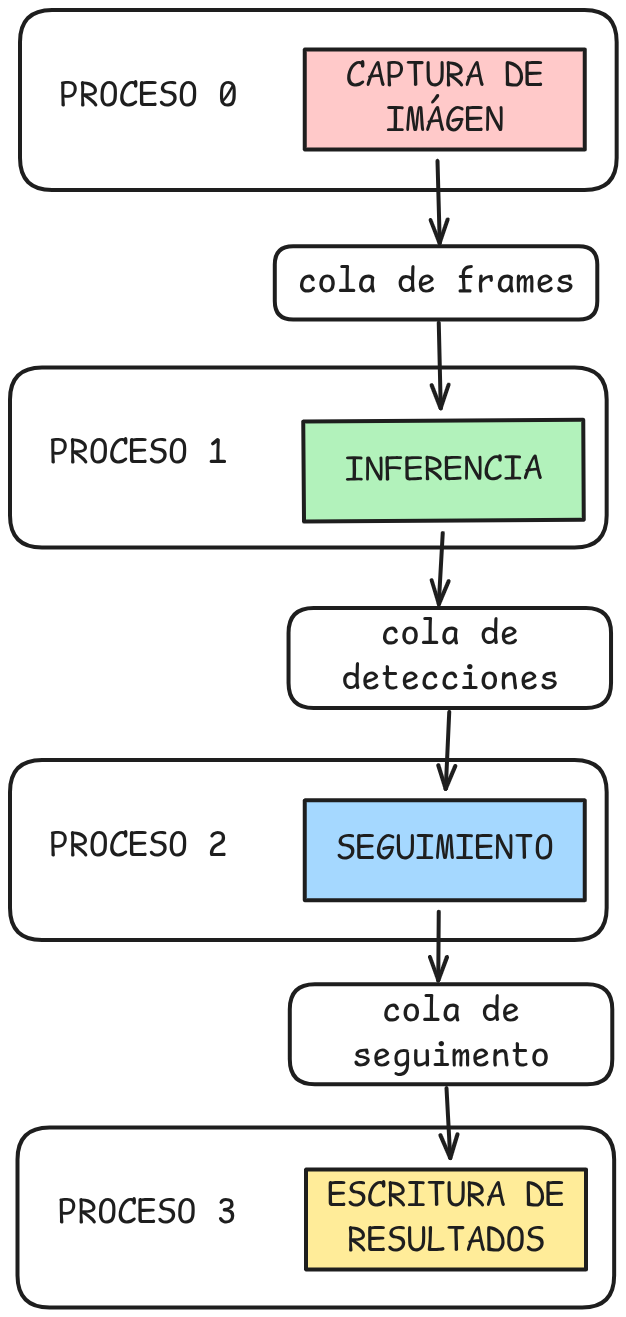
\includegraphics[width=0.3\textwidth]{images/diseno_e_implementacion/segmentacion_procesos.png}
   \caption{Diagrama de flujo del sistema segmentado en procesos.}
   \label{fig:procesos}
\end{figure}

La Figura~\ref{fig:procesos} ilustra este enfoque, donde cada etapa opera en su propio proceso y se comunica mediante colas.

Sin embargo, este enfoque también presenta desventajas. La comunicación entre procesos es más costosa en términos de tiempo y recursos que la comunicación entre hilos dentro de un mismo proceso. Además, la gestión de memoria y el intercambio de datos entre procesos pueden ser más complejos, lo que puede aumentar la dificultad de implementación y mantenimiento del sistema.

\begin{figure}[H]
   \centering
   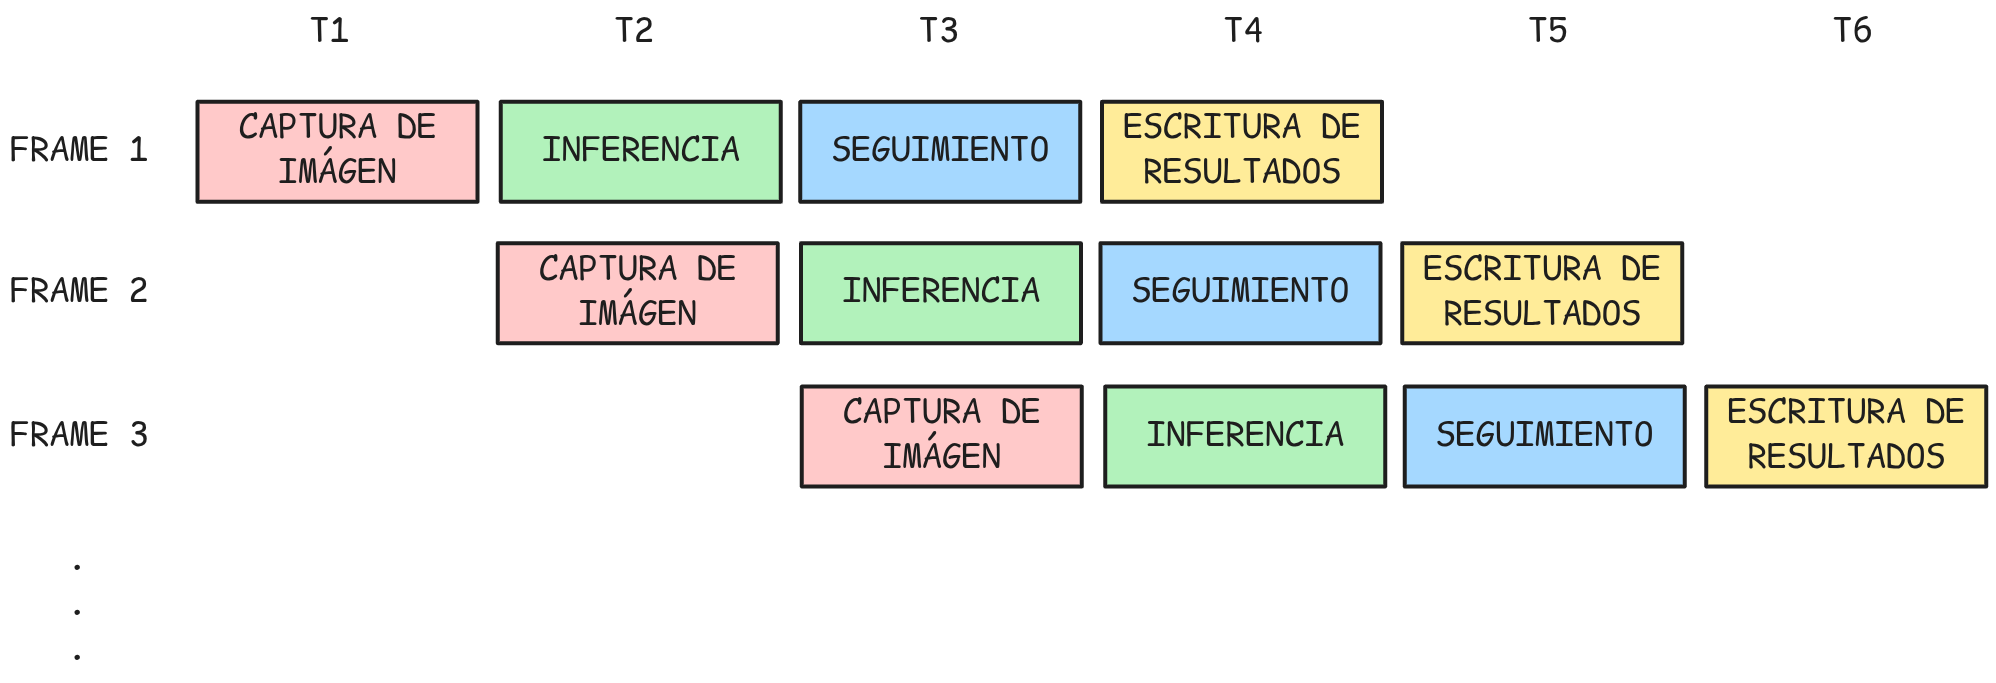
\includegraphics[width=1\textwidth]{images/diseno_e_implementacion/segmentacion.png}
   \caption{Diagrama de flujo del sistema segmentado.}
   \label{fig:segmentacion}
\end{figure}

La Figura \ref{fig:segmentacion} ilustra el flujo de datos en un sistema segmentado mediante procesos independientes, contrastando con el enfoque secuencial mostrado en la Figura \ref{fig:secuencial}. En este diseño segmentado, cada etapa principal (captura, inferencia, seguimiento, escritura) opera en su propio proceso, permitiendo la ejecución concurrente en diferentes núcleos de CPU si están disponibles.

Siguiendo la analogía con la arquitectura de un procesador, este enfoque se asemeja a un procesador segmentado (pipelined), donde diferentes instrucciones se encuentran en distintas fases de ejecución simultáneamente. Sin embargo, existe una diferencia fundamental: mientras que en un procesador segmentado todas las etapas avanzan sincronizadas por un ciclo de reloj común, determinado por la duración de la etapa más lenta, en nuestro sistema las etapas operan de forma asíncrona.

Cada etapa del sistema (captura, inferencia, seguimiento, escritura) tiene una duración variable y no necesariamente igual a las demás. Por ejemplo, la inferencia en la GPU puede ser mucho más rápida o lenta que la captura de imágenes o el seguimiento en la CPU. Las colas de mensajes actúan como buffers intermedios que desacoplan las etapas, permitiendo que cada una procese datos a su propio ritmo. Una etapa más rápida puede producir resultados que se acumulan en la cola de salida, mientras que una etapa más lenta consumirá datos de su cola de entrada cuando estén disponibles, esperando si la cola está vacía.

Esta asincronía, gestionada mediante colas, permite un mayor rendimiento (throughput) en comparación con el modelo estrictamente secuencial (Figura \ref{fig:secuencial}), donde cada etapa debe esperar a que la anterior finalice completamente. No obstante, si una etapa es significativamente más lenta que las demás, puede convertirse en un cuello de botella, haciendo que las colas anteriores se llenen y las posteriores permanezcan vacías, limitando el rendimiento general del sistema al ritmo de la etapa más lenta.


\subsection{Segmentación basada en hardware} \label{sub:segmentacion_hardware}
La cuarta opción es la segmentación basada en hardware. Aprovechando la arquitectura heterogénea de la plataforma NVIDIA Jetson, esta opción de segmentación distribuye las tareas entre las diferentes unidades de procesamiento disponibles. La etapa de inferencia, supuestamente la más exigente computacionalmente, se descarga específicamente a los aceleradores de hardware: la GPU o uno de los Deep Learning Accelerators (DLA0, DLA1) si están presentes en el módulo Jetson. Las demás etapas (captura, seguimiento y escritura) permanecen asignadas a la CPU.

Este enfoque permite una ejecución paralela real, donde la CPU gestiona el flujo de datos y la lógica de seguimiento mientras la GPU y/o las DLAs procesan simultáneamente los fotogramas para la detección de objetos. Para manejar los resultados que llegan de forma asíncrona desde estos aceleradores, a cada fotograma capturado se le asigna un identificador único. Esto garantiza que las detecciones se asocien correctamente con el fotograma original antes de pasar a la etapa de seguimiento, preservando así el orden temporal de la secuencia. La comunicación entre los procesos que se ejecutan en la CPU y aquellos que gestionan la inferencia en los aceleradores se realiza mediante las colas inter-proceso seguras (\textit{process-safe queues}) descritas anteriormente.

\begin{figure}[H]
   \centering
   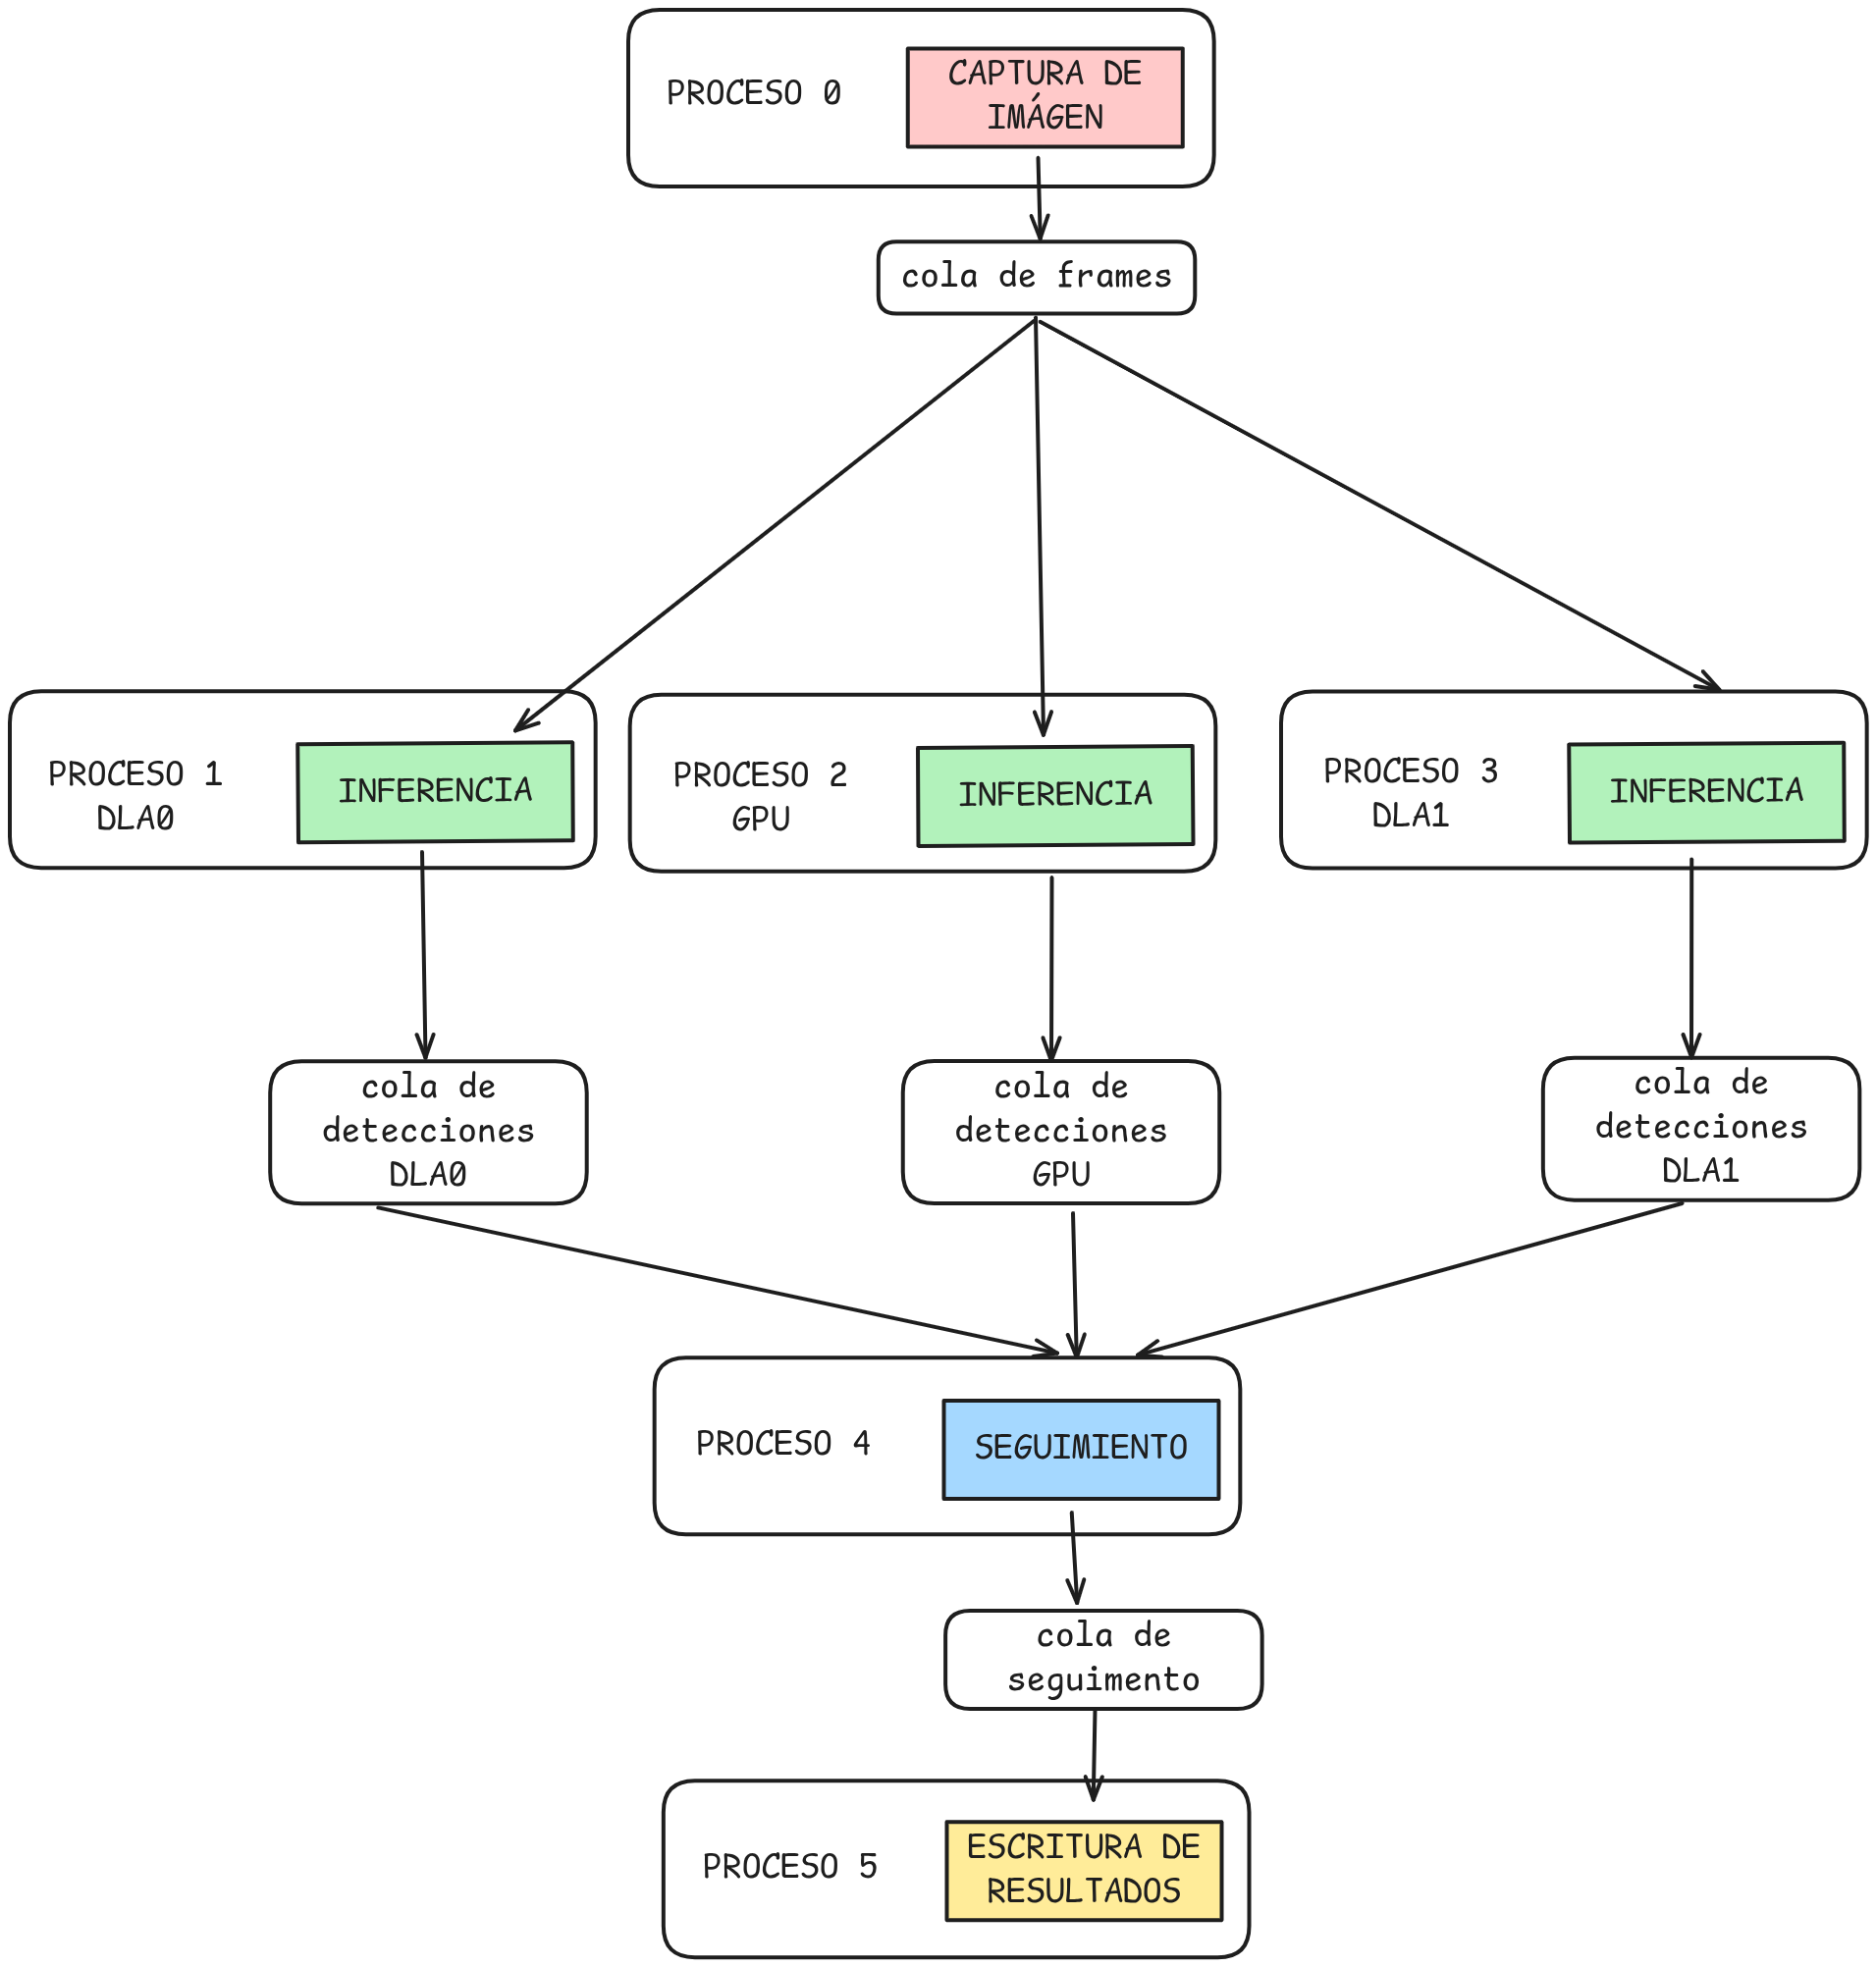
\includegraphics[width=0.6\textwidth]{images/diseno_e_implementacion/segmentacion_multihardware.png}
   \caption{Diagrama de flujo del sistema segmentado en diferentes unidades de procesamiento.}
   \label{fig:segmentacion_multihardware}
\end{figure}

La Figura \ref{fig:segmentacion_multihardware} ilustra cómo la etapa de inferencia puede ejecutarse en paralelo en la GPU o DLA, comunicándose con la etapa de seguimiento (en CPU) a través de colas. Esta distribución optimiza el uso de los recursos especializados, acelerando significativamente el rendimiento general del sistema.


\subsection{Segmentación basada en procesos con memoria compartida} \label{sub:segmentacion_memoria_compartida}


La quinta opción de segmentación emplea procesos independientes como en la sección \ref{sub:segmentacion_procesos}, pero busca optimizar la comunicación entre ellos utilizando memoria compartida como alternativa a las colas estándar del módulo \texttt{multiprocessing}. La transferencia de grandes volúmenes de datos, como los fotogramas de vídeo, puede volverse ineficiente con \texttt{multiprocessing.Queue} debido a la sobrecarga asociada a la serialización (\textit{pickling}) y deserialización de objetos, así como a la posible copia de datos entre los espacios de memoria de los procesos a través de mecanismos subyacentes como pipes.

Para superar estas limitaciones, la biblioteca \texttt{multiprocessing.shared\_memory} de Python permite a múltiples procesos acceder directamente a la misma región de memoria. Un proceso crea un bloque de memoria compartida, y otros procesos pueden adjuntarse a él usando su nombre único. Ambos pueden leer y escribir directamente en el \textit{buffer} de memoria (\texttt{shm.buf}). Este acceso directo elimina los pasos de serialización/deserialización y las copias intermedias, resultando en una latencia mucho menor y un mayor ancho de banda, lo cual es especialmente beneficioso para datos grandes y estructurados como imágenes o \textit{arrays} NumPy.


\begin{figure}[H]
   \centering
   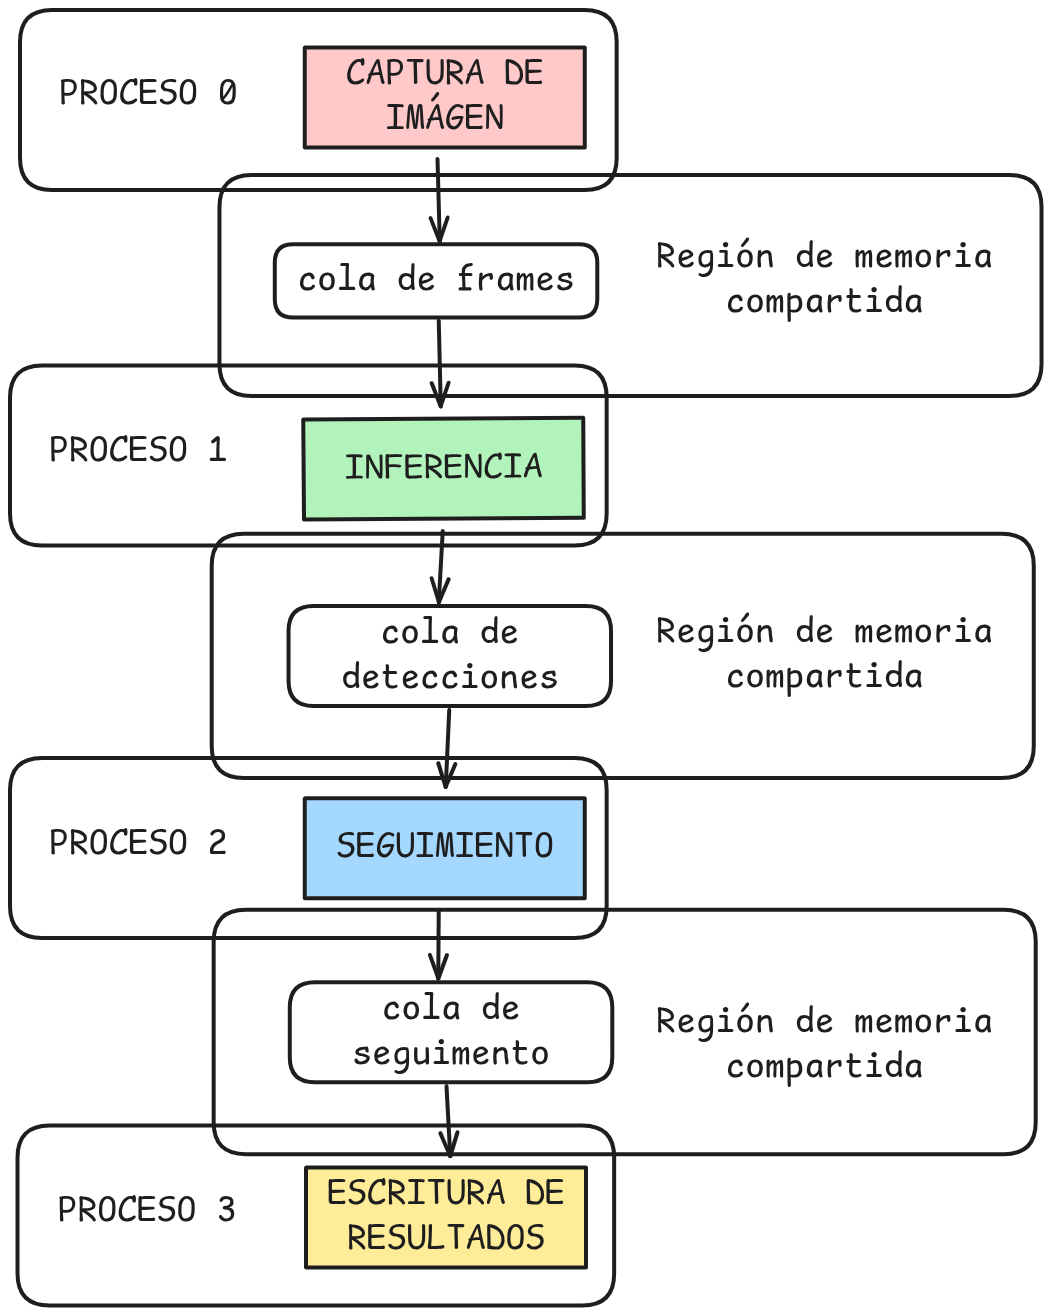
\includegraphics[width=0.5\textwidth]{images/diseno_e_implementacion/segmentacion_procesos_memoria_compartida.png}
   \caption{Diagrama de flujo del sistema segmentado en procesos con memoria compartida.}
   \label{fig:segmentacion_procesos_memoria_compartida}
\end{figure}

La Figura \ref{fig:segmentacion_procesos_memoria_compartida} ilustra este enfoque, donde cada etapa opera en su propio proceso y se comunica mediante memoria compartida. Este método permite una transferencia de datos más eficiente entre procesos, eliminando la necesidad de serialización y deserialización, lo que resulta en una latencia reducida y un mayor rendimiento general del sistema.


Sin embargo, la gestión directa de la memoria compartida requiere una implementación cuidadosa. Para facilitar su uso y gestionar el flujo de datos de manera estructurada, se ha implementado una capa de abstracción: un buffer circular. Este buffer opera sobre un bloque de memoria compartida preasignado y funciona como una cola de capacidad fija. Los datos se escriben en una posición (\textit{tail}) y se leen desde otra (\textit{head}). Cuando los índices alcanzan el final del \textit{buffer}, vuelven al principio, permitiendo un uso continuo del espacio de memoria. La Figura \ref{fig:buffer_circular} ilustra esta estructura conceptual.

\begin{figure}[H]
   \centering
   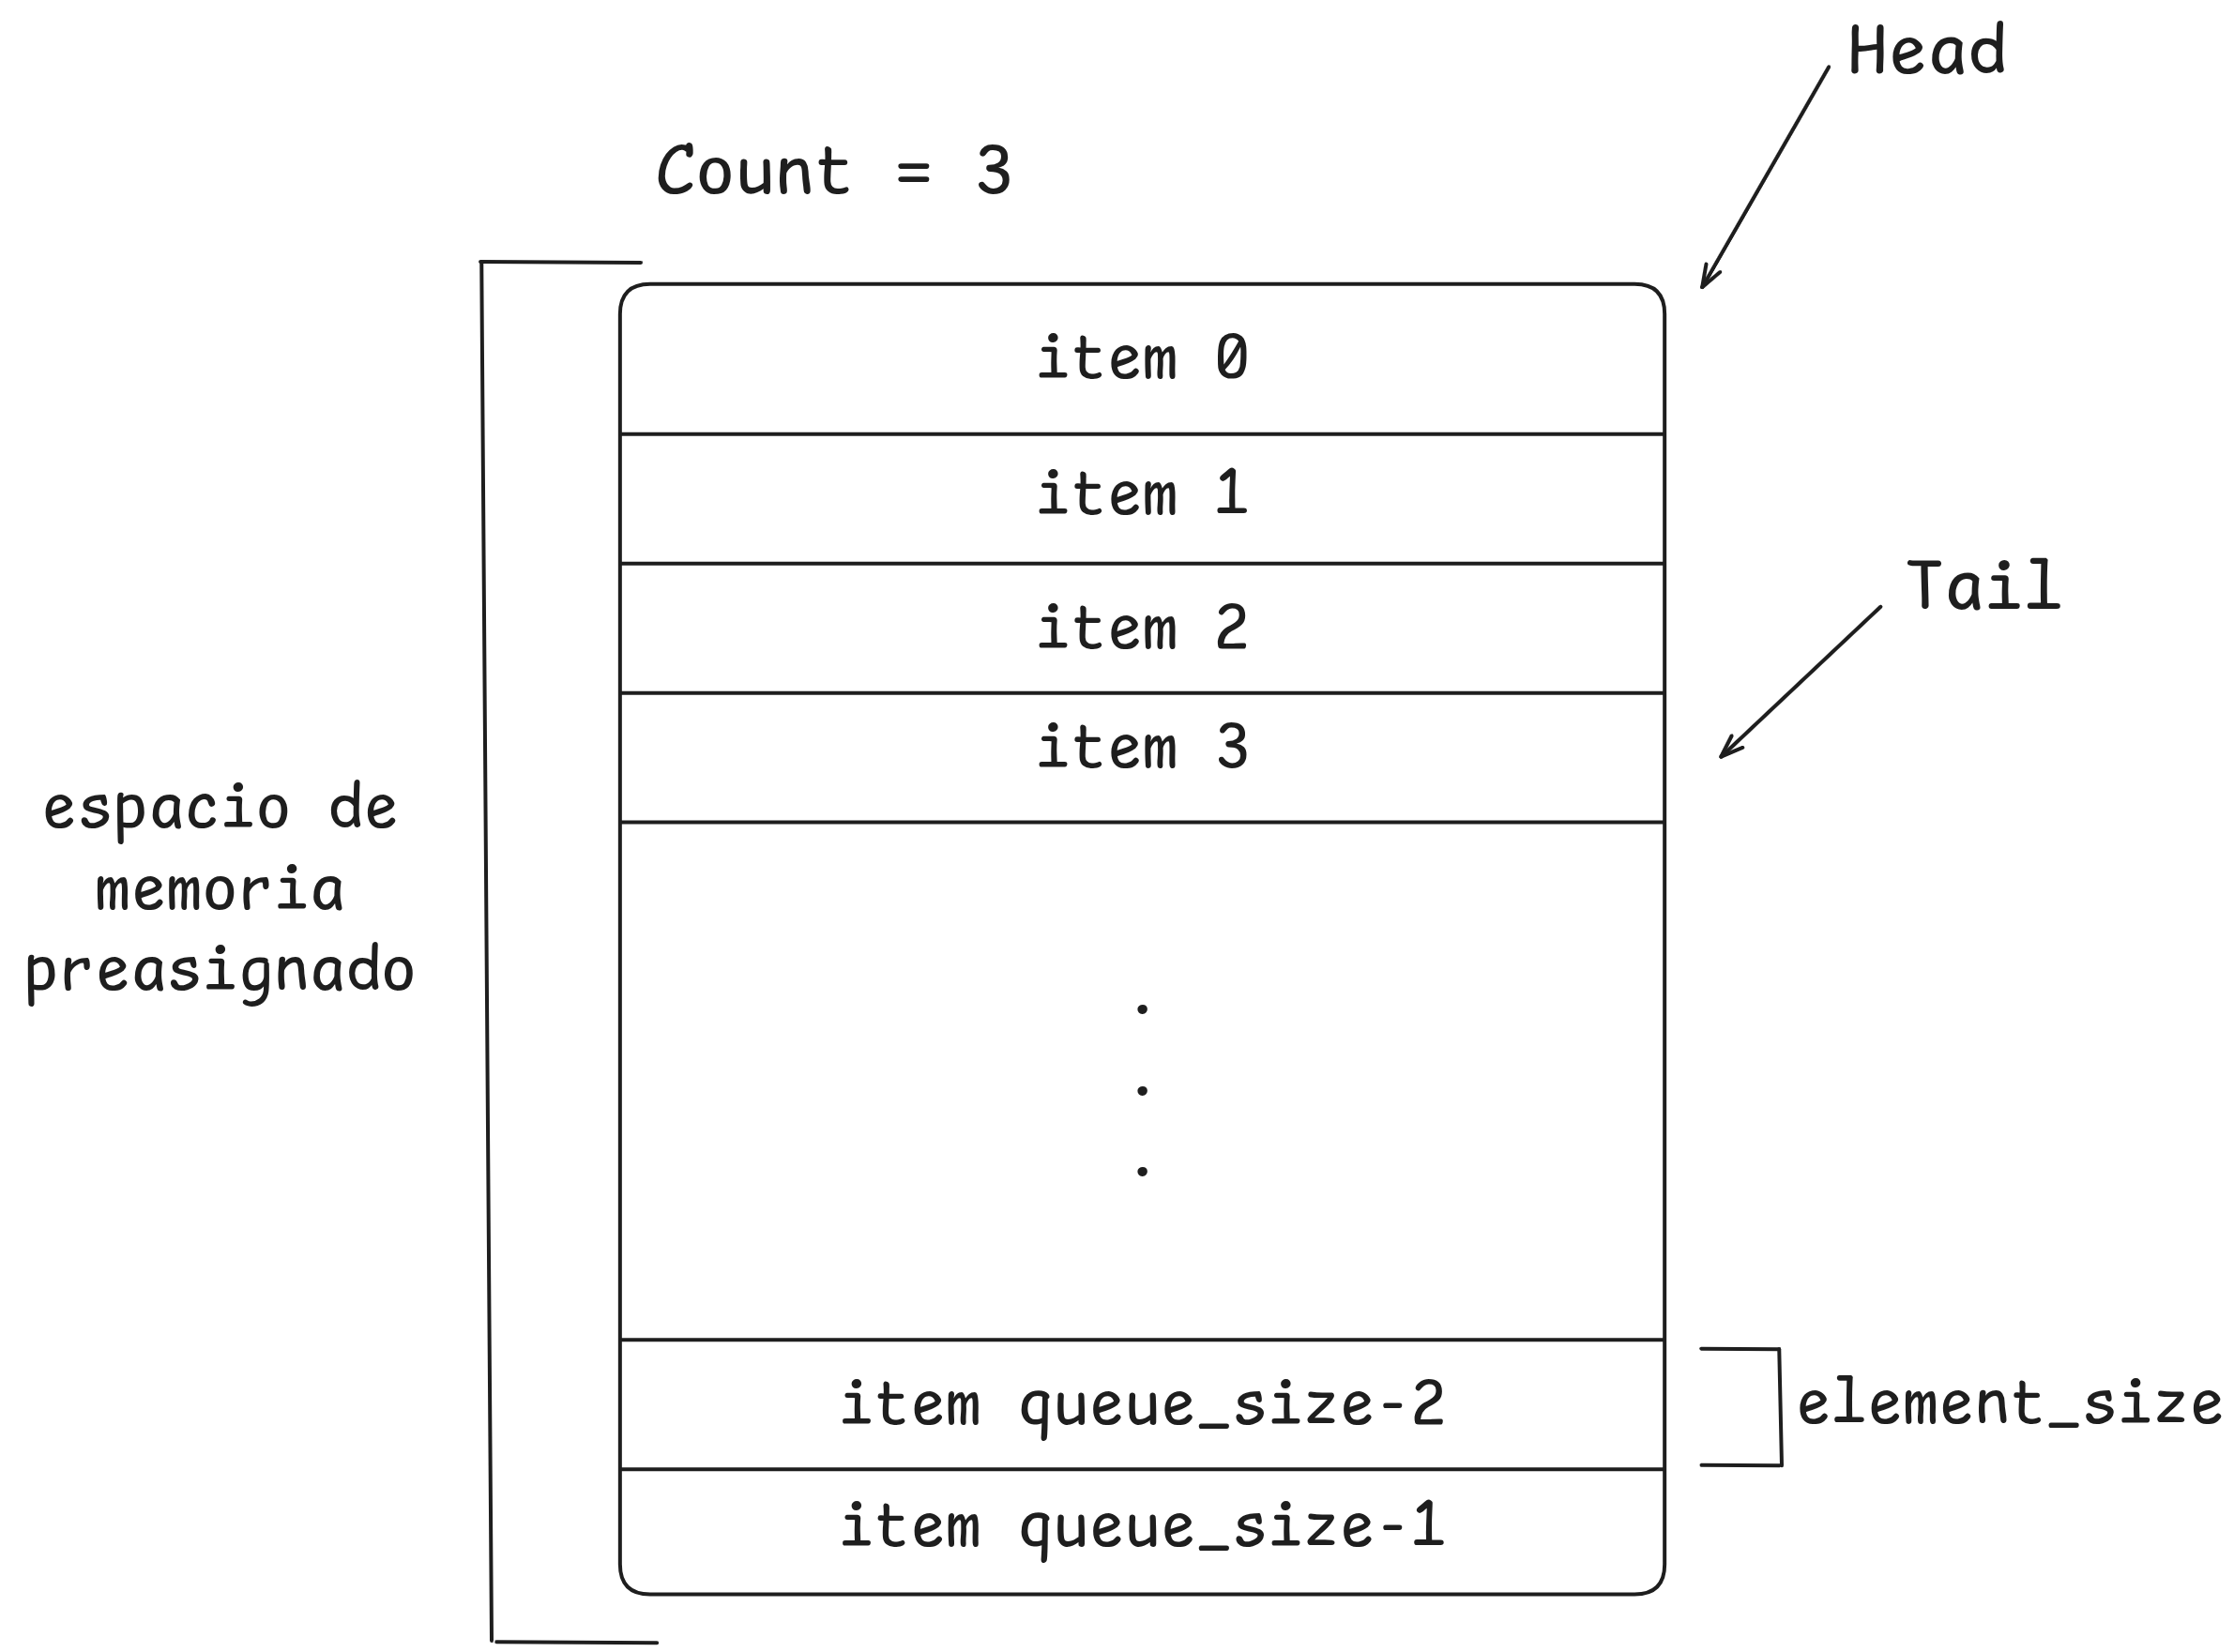
\includegraphics[width=0.6\textwidth]{images/diseno_e_implementacion/buffer_circular.png}
   \caption{Ejemplo de buffer circular.}
   \label{fig:buffer_circular}
\end{figure}

Dado que múltiples procesos acceden concurrentemente a la misma memoria a través del \textit{buffer} circular, es crucial garantizar la coherencia de los datos y prevenir condiciones de carrera. A diferencia de \texttt{multiprocessing.Queue}, que gestiona la sincronización internamente, \texttt{shared\_memory} no la proporciona automáticamente. Por lo tanto, el \textit{buffer} circular implementado integra mecanismos de sincronización explícitos, como bloqueos (\textit{Lock}) y variables de condición (\textit{Semaphore}) del módulo \texttt{multiprocessing}. Estos controlan el acceso: un proceso productor que intente añadir datos a un buffer lleno se bloqueará hasta que un consumidor libere espacio, y viceversa, un consumidor que intente leer de un buffer vacío esperará. Este comportamiento asegura que no se pierdan datos y que las operaciones se realicen de forma segura.

La configuración de cada buffer circular requiere definir estáticamente su capacidad, el tamaño de memoria para cada elemento y un nombre único para la región de memoria compartida. Una limitación clave es la necesidad de preasignar la memoria. Una asignación incorrecta (demasiado grande o demasiado pequeña) puede llevar a desperdicio de recursos o a bloqueos frecuentes que limiten el rendimiento. Por ello, se requiere una calibración experimental para determinar los tamaños óptimos de buffer para cada enlace entre etapas, buscando el equilibrio entre uso eficiente de memoria y fluidez en el procesamiento. Además, el programador debe gestionar manualmente el ciclo de vida del bloque de memoria compartida (creación, cierre con \texttt{close()} y liberación final con \texttt{unlink()}).

En resumen, la segmentación basada en procesos con memoria compartida y un buffer circular busca ofrecer un rendimiento superior para la transferencia de grandes bloques de datos como fotogramas de vídeo, aunque esto implicaría una mayor complejidad en la implementación y gestión de la memoria.


\chapter{Evaluación de la solución} \label{chap:evaluacion_solucion}

En este capítulo se presenta la evaluación del sistema propuesto, analizando su rendimiento y eficiencia en diferentes configuraciones. Se describen las metodologías de evaluación empleadas, las métricas de rendimiento consideradas y los resultados obtenidos en cada caso. El objetivo es proporcionar una visión clara de cómo el sistema se comporta bajo diversas condiciones y configuraciones, permitiendo identificar sus fortalezas y áreas de mejora.

\section{Metodología de evaluación y métricas de rendimiento} \label{sec:metodologia}

Tras el desarrollo de la solución propuesta, se procede a analizar su rendimiento. La evaluación se basa en diferentes vídeos de prueba de 80 segundos (2400 fotogramas) que muestran un flujo de canicas, grabados a 640x640 píxeles y 30 fotogramas por segundo. Estos vídeos sirven como entrada estándar para el sistema, permitiendo medir diversas métricas de rendimiento según la configuración.

Para evaluar el rendimiento del sistema, se han implementado dos metodologías de ejecución:

\begin{enumerate}
   \item \textbf{Ejecución a máxima capacidad:} Los fotogramas se entregan al sistema consecutivamente, tan pronto como el procesamiento del fotograma anterior ha concluido, utilizando colas intermedias que no descartan fotogramas. En este escenario, se mide el tiempo total que el sistema tarda en procesar la secuencia completa, lo que permite evaluar su rendimiento máximo (throughput) y compararlo con la duración real del vídeo.
   \item \textbf{Simulación de entrada en tiempo real:} Los fotogramas del vídeo se suministran al sistema a una tasa fija de 30 fps (un fotograma cada 33.3 ms), emulando la entrada de una cámara. Si el sistema no logra procesar un fotograma dentro de este intervalo, dicho fotograma se descarta. Esta metodología permite cuantificar la capacidad del sistema para operar en tiempo real, midiendo el número de fotogramas procesados y perdidos.
\end{enumerate}

Como métricas de rendimiento, se han considerado las siguientes:
\begin{itemize}
   \item \textbf{Tasa de fotogramas por segundo (FPS):} Número de fotogramas completamente procesados por segundo. Esta métrica es fundamental para evaluar la capacidad del sistema para operar en tiempo real, ya que cuantifica directamente su velocidad de procesamiento. Un valor mayor o igual a 30 FPS generalmente indica que el sistema puede funcionar en tiempo real para vídeos estándar.

      \item \textbf{Tasa de fotogramas perdidos (LFPS):} Número de fotogramas descartados por segundo debido a la incapacidad del sistema para procesarlos dentro del intervalo temporal requerido. Esta métrica refleja la robustez del sistema bajo restricciones de tiempo real y su eficacia para mantener sincronización con la fuente de entrada. Un valor cercano a cero indica un rendimiento óptimo.

      \item \textbf{Potencia media consumida (W):} Potencia eléctrica media requerida por el sistema durante la ejecución, medida en vatios. Se obtiene promediando las lecturas de potencia instantánea registradas por las herramientas de monitorización hardware. Esta métrica es crucial para evaluar la viabilidad del sistema en entornos con restricciones energéticas, especialmente en aplicaciones \textit{embedded} o en el \textit{edge}.

      \item \textbf{Energía consumida (J):} Cantidad total de energía eléctrica utilizada por el sistema para procesar la secuencia completa, medida en julios. Se calcula integrando la potencia instantánea a lo largo del tiempo de ejecución. Esta métrica proporciona una perspectiva integral de la eficiencia energética y es fundamental para estimar costes operativos y requisitos de refrigeración en implementaciones a largo plazo.

      \item \textbf{Fotogramas por vatio (Frames/W):} Métrica compuesta que indica la eficiencia energética del procesamiento, cuantificando cuántos fotogramas se procesan por cada vatio de potencia consumida. Permite comparar directamente configuraciones con diferentes compromisos entre velocidad y consumo. Se calcula mediante la siguiente relación:
      \begin{equation}
         \text{FPS/W} = \frac{\text{Frames procesados}}{\text{Potencia (W)} \cdot \text{Tiempo (s)}}
      \end{equation}
      donde
      \begin{equation}
         \text{Energía consumida (J)} = \text{Potencia (W)} \cdot \text{Tiempo (s)}
      \end{equation}
      por lo tanto
      \begin{equation}
         \text{FPS/W} = \frac{\text{Frames procesados}}{\text{Energía consumida (J)}}
      \end{equation}
      
      \item \textbf{Speedup:} Factor de aceleración que cuantifica la mejora relativa en velocidad de procesamiento. Se calcula como el cociente entre el tiempo de ejecución de la configuración de referencia (generalmente la más lenta) y el tiempo de la configuración evaluada. Un valor de 2.0 indicaría que la configuración actual es exactamente dos veces más rápida que la referencia. Esta métrica permite evaluar objetivamente los beneficios de optimizaciones específicas.

      \item \textbf{GPU Average Utilization:} Porcentaje medio de utilización de los recursos de la GPU durante el tiempo de ejecución. Este valor, obtenido mediante las herramientas de monitorización de NVIDIA, representa qué fracción de la capacidad computacional total de la GPU se aprovecha efectivamente. Una utilización cercana al 100\% sugiere un aprovechamiento óptimo del hardware, mientras que valores bajos podrían indicar cuellos de botella en otras partes del sistema o ineficiencias en la implementación.
      
      \item \textbf{CPU Average Utilization:} Porcentaje medio de utilización de los núcleos de la CPU durante el tiempo de ejecución. Esta métrica es la media aritmética de todos los núcleos disponibles (entre 1 y 12, dependiendo de la configuración específica del dispositivo Jetson) y lo promedia. Permite identificar si las etapas del sistema que se ejecutan en CPU están equilibradas respecto a las que utilizan aceleradores hardware, y detectar posibles desbalances en la carga de trabajo entre las diferentes unidades de procesamiento.

\end{itemize}


Para obtener estas métricas, se han utilizado herramientas de medición de potencia y energía, como el comando \texttt{tegrastats} de NVIDIA, que proporciona información sobre el consumo de energía y la carga de la CPU y GPU. Esta herramienta permite monitorizar el rendimiento del sistema en tiempo real, proporcionando datos precisos sobre el uso de recursos y el consumo energético.

\section{Cantidad de objetos} \label{sec:cantidad_objetos}
La cantidad de objetos presentes en el flujo de vídeo es un factor determinante en la evaluación del rendimiento del sistema, ya que influye directamente en la carga computacional de la etapa de seguimiento y escritura. Para analizar esta influencia de manera sistemática, se han realizado pruebas utilizando tres vídeos de prueba distintos, cada uno diseñado para representar un escenario de carga diferente:
\begin{enumerate}


   \item \textbf{Vídeo 1: Carga baja y constante:} Un vídeo que mantiene una cantidad constante baja de 17 objetos en cada fotograma. Este escenario permite evaluar el rendimiento base del sistema bajo una carga predecible y reducida.
   \item \textbf{Vídeo 2: Carga media y constante:} Un vídeo que presenta una cantidad constante media de 43 objetos por fotograma. Este escenario permite observar el rendimiento del sistema bajo una carga moderada.
   \item \textbf{Vídeo 3: Carga alta y constante:} Un vídeo que presenta una cantidad constante media de 84 objetos por fotograma. Este escenario somete al sistema a una carga significativamente mayor, permitiendo identificar posibles cuellos de botella bajo condiciones de alta densidad de objetos.
   \item \textbf{Vídeo 4: Carga variable:} Un vídeo donde la cantidad de objetos fluctúa dinámicamente a lo largo de su duración, variando entre un mínimo de 0 y un máximo de 180 objetos. Este escenario simula condiciones más realistas y complejas, donde el sistema debe adaptarse a cambios abruptos en la carga de trabajo.
\end{enumerate}
Todos los vídeos de prueba se grabaron con una resolución de 640x640 píxeles y a una tasa de 30 fotogramas por segundo, sirviendo como entrada estándar para el sistema, lo que asegura la consistencia en las condiciones de captura.

Para el resto de la configuración del sistema durante estas pruebas específicas sobre la cantidad de objetos, se ha empleado la segmentación por procesos con memoria compartida. El modelo de detección de objetos utilizado fue YOLO11n, optimizado mediante NVIDIA TensorRT para su ejecución en la GPU.

Se configuró para operar con precisión FP16 y con el perfil de energía del dispositivo Jetson ajustado al modo de máxima potencia (MAXN). Esta configuración se seleccionó con el objetivo de maximizar el rendimiento del sistema y evaluar su capacidad de respuesta y robustez bajo condiciones exigentes impuestas por la variación en la densidad de objetos.

Las pruebas que se presentan a continuación se realizaron siguiendo la metodología de ejecución a máxima capacidad descrita en la sección \ref{sec:metodologia}, donde los fotogramas se entregan al sistema consecutivamente, tan pronto como el procesamiento del fotograma anterior ha concluido, utilizando colas intermedias que no descartan fotogramas. En este escenario, se mide el tiempo total que el sistema tarda en procesar la secuencia completa, lo que permite evaluar su rendimiento máximo (throughput) y compararlo con la duración real del vídeo.

\begin{figure}[H]
   \centering
   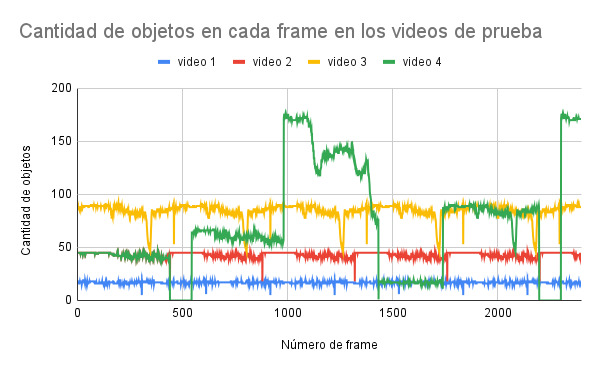
\includegraphics[width=0.8\textwidth]{images/analisis_de_la_solucion/cantidad_objetos/cantidad_objetos_4_videos.png}
   \caption{Cantidad de objetos en los vídeos de prueba.}
   \label{fig:4_videos}
\end{figure}

La Figura \ref{fig:4_videos} ilustra la cantidad de objetos presentes en cada fotograma para los cuatro vídeos de prueba utilizados: carga baja constante (17 objetos), carga media constante (43 objetos), carga alta constante (84 objetos) y carga variable (entre 0 y 180 objetos).

\begin{figure}[H]
   \centering
   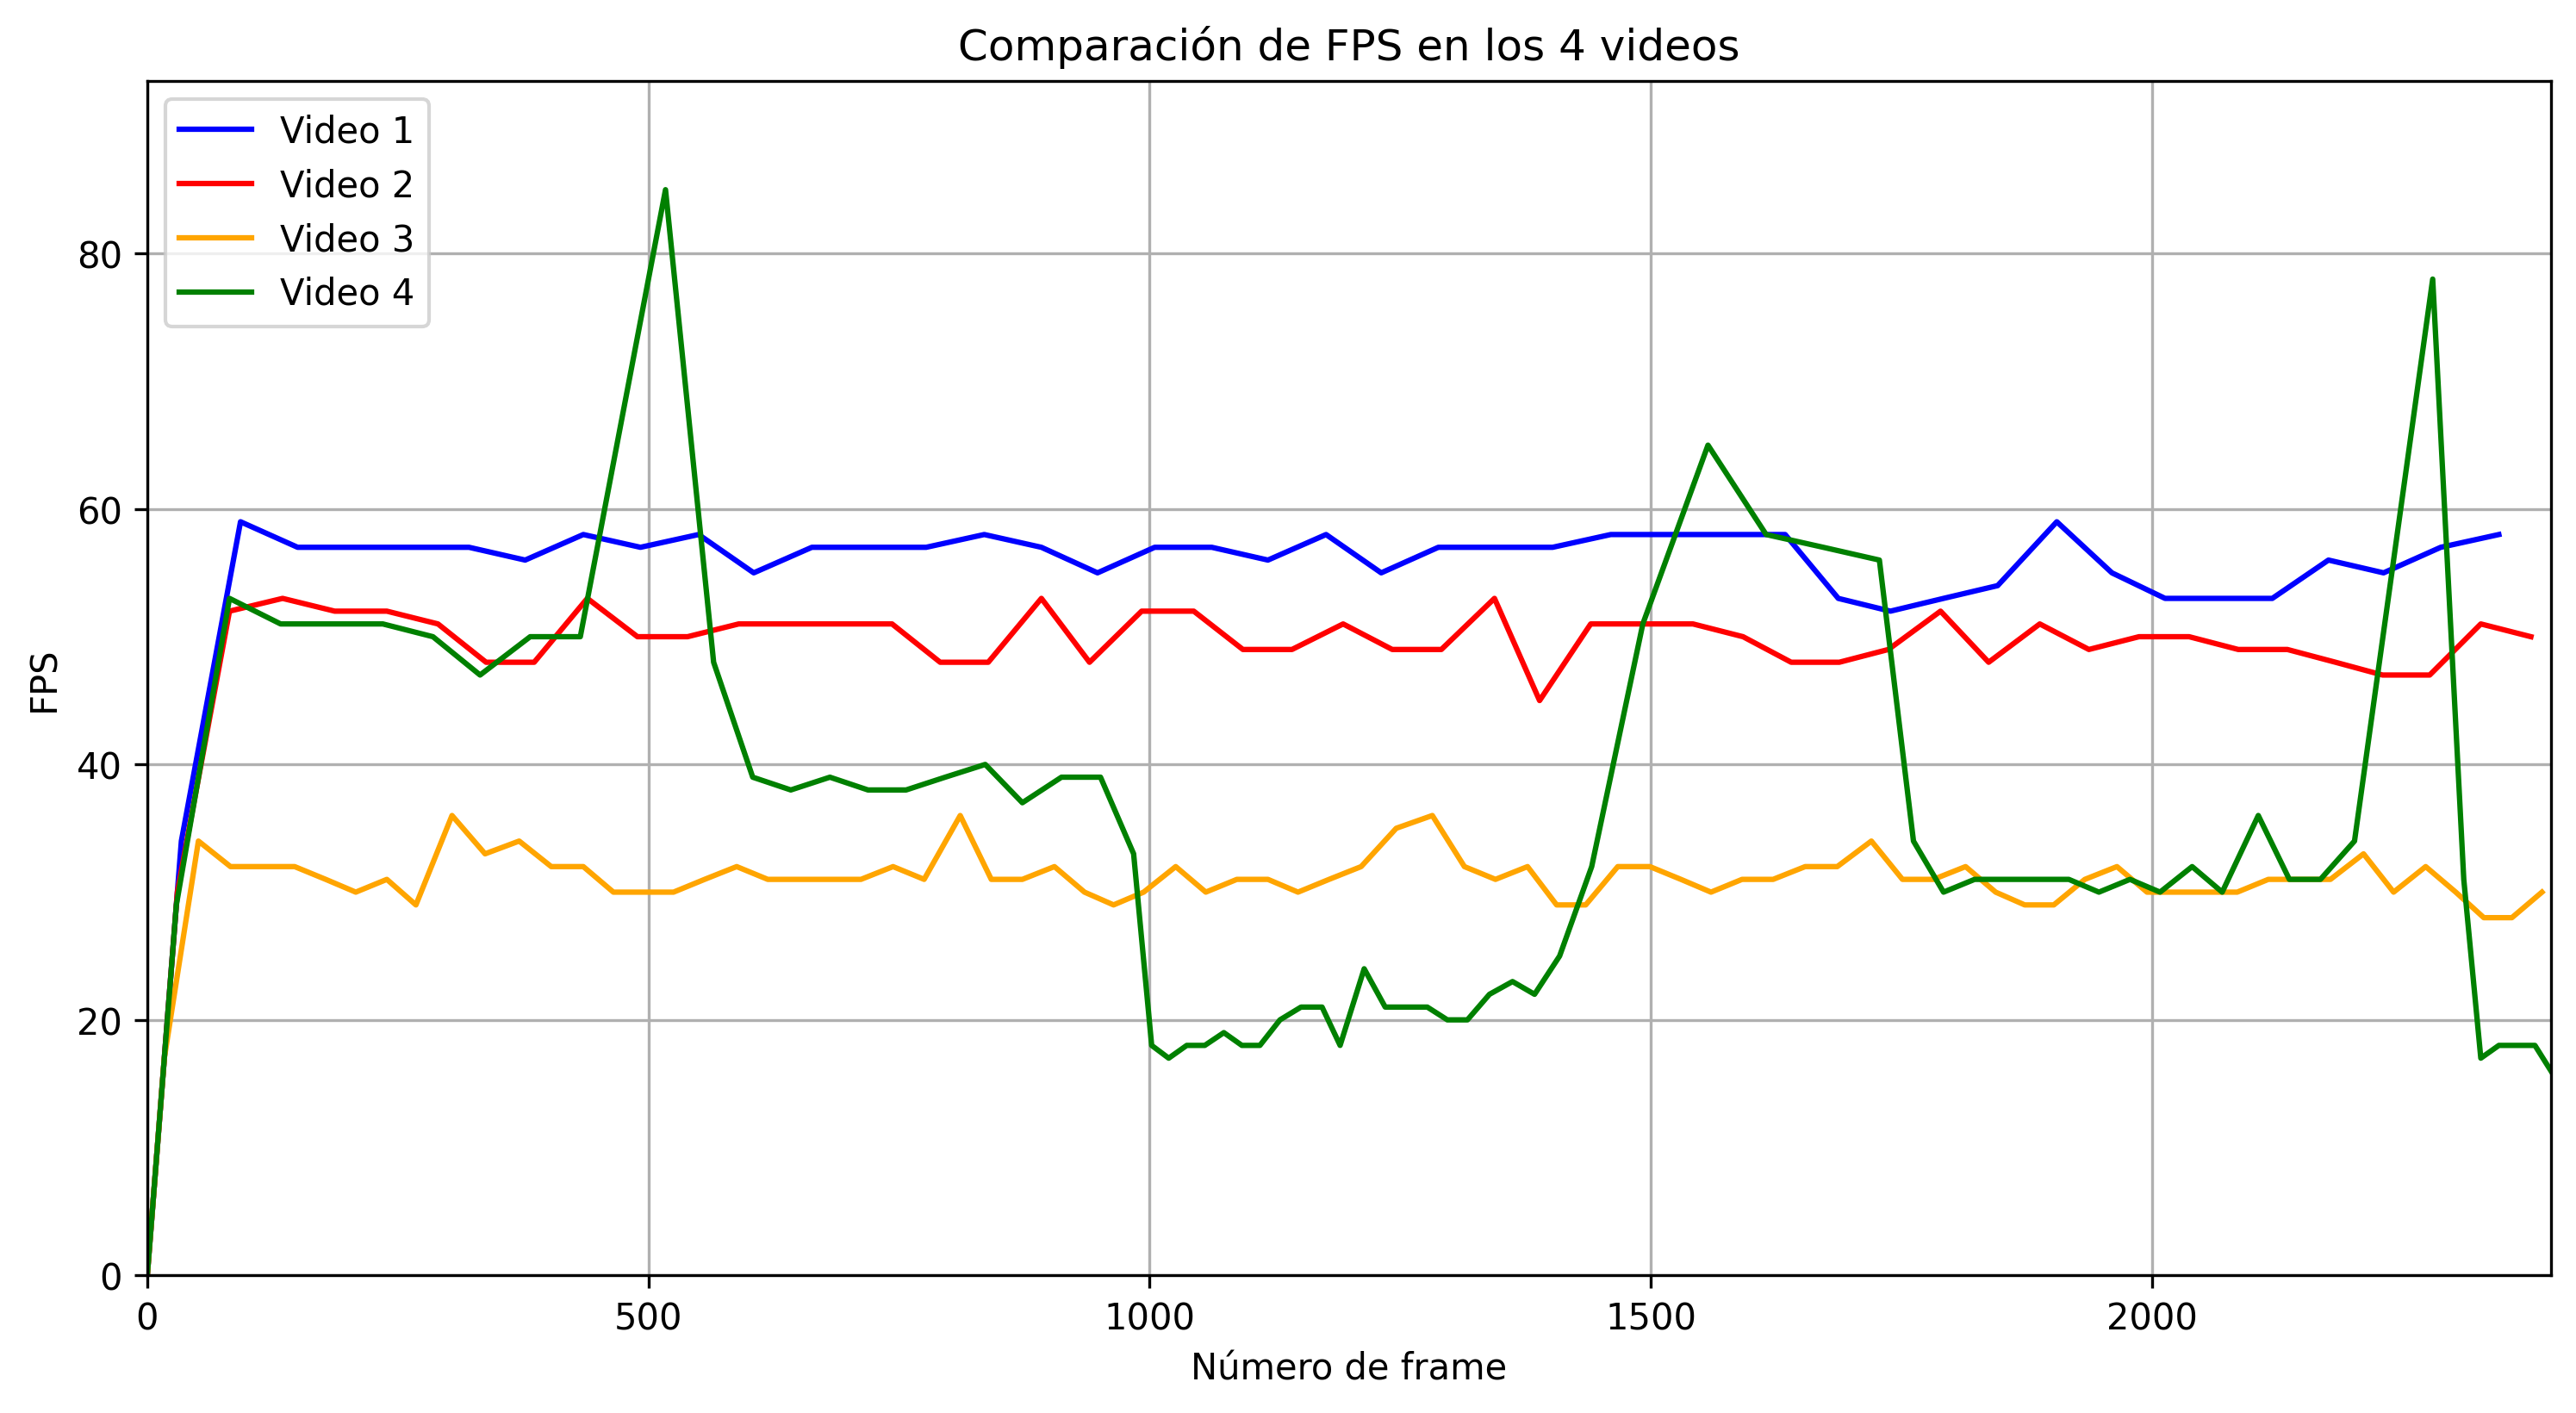
\includegraphics[width=0.8\textwidth]{excels/inferencia/cantidad_objetos/resultados/max_fps_4_videos/fps_comparison.png}
   \caption{FPS por fotograma en función de la cantidad de objetos para los cuatro vídeos de prueba.}
   \label{fig:fps_por_frame}
\end{figure}

Al examinar la Figura \ref{fig:fps_por_frame}, se evidencia una clara correlación entre el rendimiento del sistema, cuantificado en fotogramas por segundo (FPS), y la densidad de objetos presentes en el flujo de vídeo. En el escenario de carga baja y constante (línea azul), el sistema mantiene un rendimiento consistente y elevado, oscilando entre 50-60 FPS. Para el vídeo de carga media y constante (línea roja), se observa una ligera degradación del rendimiento, que se estabiliza en el rango de 45-50 FPS. En condiciones de carga alta y constante (línea amarilla), el rendimiento experimenta una reducción más significativa, estableciéndose en un promedio de 30-40 FPS. Esta progresiva disminución del rendimiento se alinea con las expectativas teóricas, dado que el incremento en la cantidad de objetos aumenta proporcionalmente la carga computacional en las etapas de seguimiento y escritura.

El escenario de carga variable (línea verde) revela un comportamiento particularmente informativo: el sistema alcanza picos superiores a 60 FPS durante intervalos con menos de 20 objetos, pero experimenta una pronunciada caída hasta aproximadamente 20 FPS cuando la densidad supera los 100 objetos. Esta marcada fluctuación en el rendimiento confirma la sensibilidad de determinadas etapas del sistema al volumen de objetos procesados simultáneamente, lo que resulta crucial para comprender sus limitaciones operativas en entornos dinámicos.

\begin{figure}[H]
   \centering
   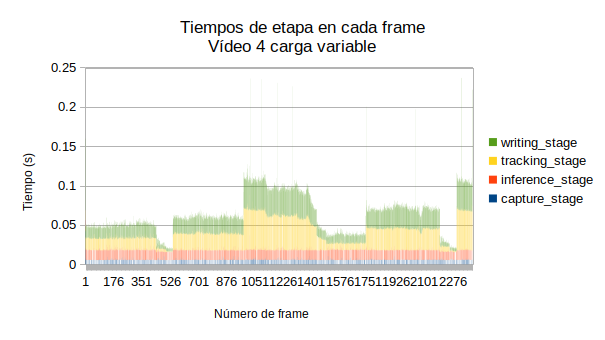
\includegraphics[width=0.8\textwidth]{images/analisis_de_la_solucion/tiempos_etapa.png}
   \caption{Ejecución temporal de las etapas del sistema durante el vídeo de prueba con carga variable.}
   \label{fig:tiempos_etapa}
\end{figure}

Para comprender a fondo el impacto de esta variación en la cantidad de objetos, es esencial analizar cómo afecta a cada etapa dentro de la arquitectura segmentada del sistema. La Figura \ref{fig:tiempos_etapa} presenta el tiempo de ejecución de cada etapa del sistema a lo largo del vídeo de prueba con carga variable.

Se observa que la etapa de captura (línea azul) se mantiene constante, ya que sus operaciones (adquisición de fotogramas) no dependen del contenido de la imagen. De manera similar, la etapa de inferencia (línea roja), ejecutada en la GPU, muestra un tiempo de procesamiento relativamente estable. Aunque podría esperarse una ligera variación, el modelo YOLO procesa la imagen completa y su carga principal no escala linealmente con el número de objetos detectados una vez que la imagen está en la GPU.

Por el contrario, la etapa de seguimiento (línea amarilla), que se ejecuta en la CPU, muestra una clara correlación entre su tiempo de ejecución y la cantidad de objetos. A medida que aumenta el número de objetos (como se ve en la curva de carga variable de la Figura \ref{fig:4_videos}), el tiempo que tarda la etapa de seguimiento también aumenta significativamente. Esto se debe a que el algoritmo BYTETrack debe gestionar más trayectorias, realizar más comparaciones para la asociación de datos y actualizar más filtros de Kalman. Este comportamiento indica que la etapa de seguimiento puede convertirse en un cuello de botella cuando la densidad de objetos es alta.

Finalmente, la etapa de escritura (línea verde), también dependiente de la CPU, muestra un ligero incremento en su tiempo de ejecución a medida que aumenta el número de objetos. Esto es esperable, ya que debe procesar y registrar la información de un mayor número de detecciones y trayectorias.


\begin{figure}[H]
   \centering
   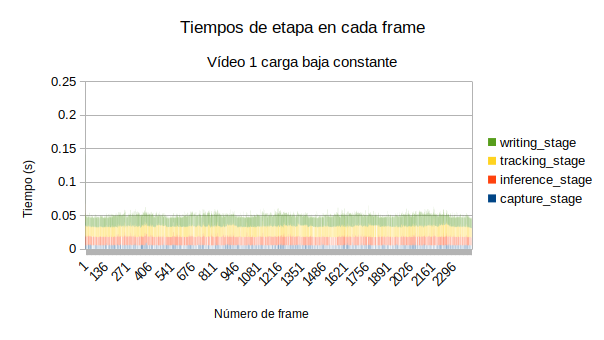
\includegraphics[width=0.8\textwidth]{images/analisis_de_la_solucion/tiempos_etapa_video1.png}
   \caption{Ejecución temporal de las etapas del sistema durante el vídeo de prueba 2 (carga media y constante).}
   \label{fig:tiempos_etapa_video1}
\end{figure}

Por otro lado, la Figura \ref{fig:tiempos_etapa_video1} muestra el tiempo de ejecución de cada etapa del sistema a lo largo del vídeo de prueba 2 (carga media y constante).

En este caso, la etapa de seguimiento (línea amarilla) presenta un tiempo de ejecución bajo y estable, reflejando la menor carga de trabajo al procesar un número constante de objetos. Esto indica que el sistema gestiona eficientemente escenarios de carga baja y media, sin generar cuellos de botella significativos en las etapas de seguimiento o escritura.

De forma similar, la etapa de escritura (línea verde) muestra tiempos de ejecución bajos y uniformes, lo que confirma la capacidad del sistema para mantener un rendimiento constante en condiciones de carga moderada.

La etapa de captura (línea azul) y la etapa de inferencia (línea roja) mantienen un rendimiento estable, similar al observado en el vídeo de carga variable, lo que indica que su rendimiento no se ve afectado por la cantidad de objetos presentes.



Ahora vamos a analizar el rendimiento del sistema con una simulación de entrada en tiempo real. En este caso, el sistema debe procesar cada fotograma en un tiempo máximo de 33.3 ms (30 fps). Si no logra hacerlo, el fotograma se descarta. Esta metodología permite evaluar la capacidad del sistema para operar en tiempo real y medir la tasa de fotogramas perdidos (LFPS).

\begin{table}[H]
   \centering
   \resizebox{\textwidth}{!}{ % Ajusta al ancho de página
   \pgfplotstabletypeset[
       col sep=comma,
       header=true,
       columns={cantidad_objetos,frames_procesados,tiempo_ejecucion_s,FPS,LFPS,potencia_media_consumida_W,energia_consumida_J,frames_por_W,avg_GPU,avg_CPU},
       display columns/0/.style={column name=Cant.\ Objetos, column type={c}, string type},
       display columns/1/.style={column name=Frames Procesados, column type={c}},
       display columns/2/.style={column name=Tiempo Ejec. (s), column type={c}},
       display columns/3/.style={column name=FPS, column type={c}},
       display columns/4/.style={column name=LFPS, column type={c}, fixed, precision=2},
       display columns/5/.style={column name=Potencia media (W), column type={c}, fixed, precision=2},
       display columns/6/.style={column name=Energía (J), column type={c}, fixed, precision=0},
       display columns/7/.style={column name=Frames/W, column type={c}},
       display columns/8/.style={column name=GPU Avg., column type={c}},
       display columns/9/.style={column name=CPU Avg., column type={c}},
       every head row/.style={before row=\toprule, after row=\midrule},
       every last row/.style={after row=\bottomrule},
       empty cells with={NaN}
   ]{excels/inferencia/cantidad_objetos/resultados/30_fps/datos.csv}
   }
   \caption{Resultados del experimento con distintas cantidades de objetos.}
   \label{tab:experimento_objetos}
\end{table}

Los datos de la Tabla \ref{tab:experimento_objetos} revelan que el sistema logra procesar una cantidad considerable de fotogramas en tiempo real bajo distintas condiciones de carga. Sin embargo, la Figura \ref{fig:fps_vs_object_count} muestra una relación más compleja: cuando la cantidad de objetos excede el umbral de 100, el rendimiento del sistema disminuye notablemente, llegando a generar tasas de fotogramas perdidos (LFPS) de hasta 10 frames por segundo en estos segmentos de alta densidad. Esta observación pone de manifiesto que las métricas promedio pueden resultar engañosas, ya que tienden a ocultar intervalos críticos de bajo rendimiento durante los picos de carga, precisamente cuando el sistema sería más necesario en aplicaciones industriales reales.

\begin{figure}
   \centering
   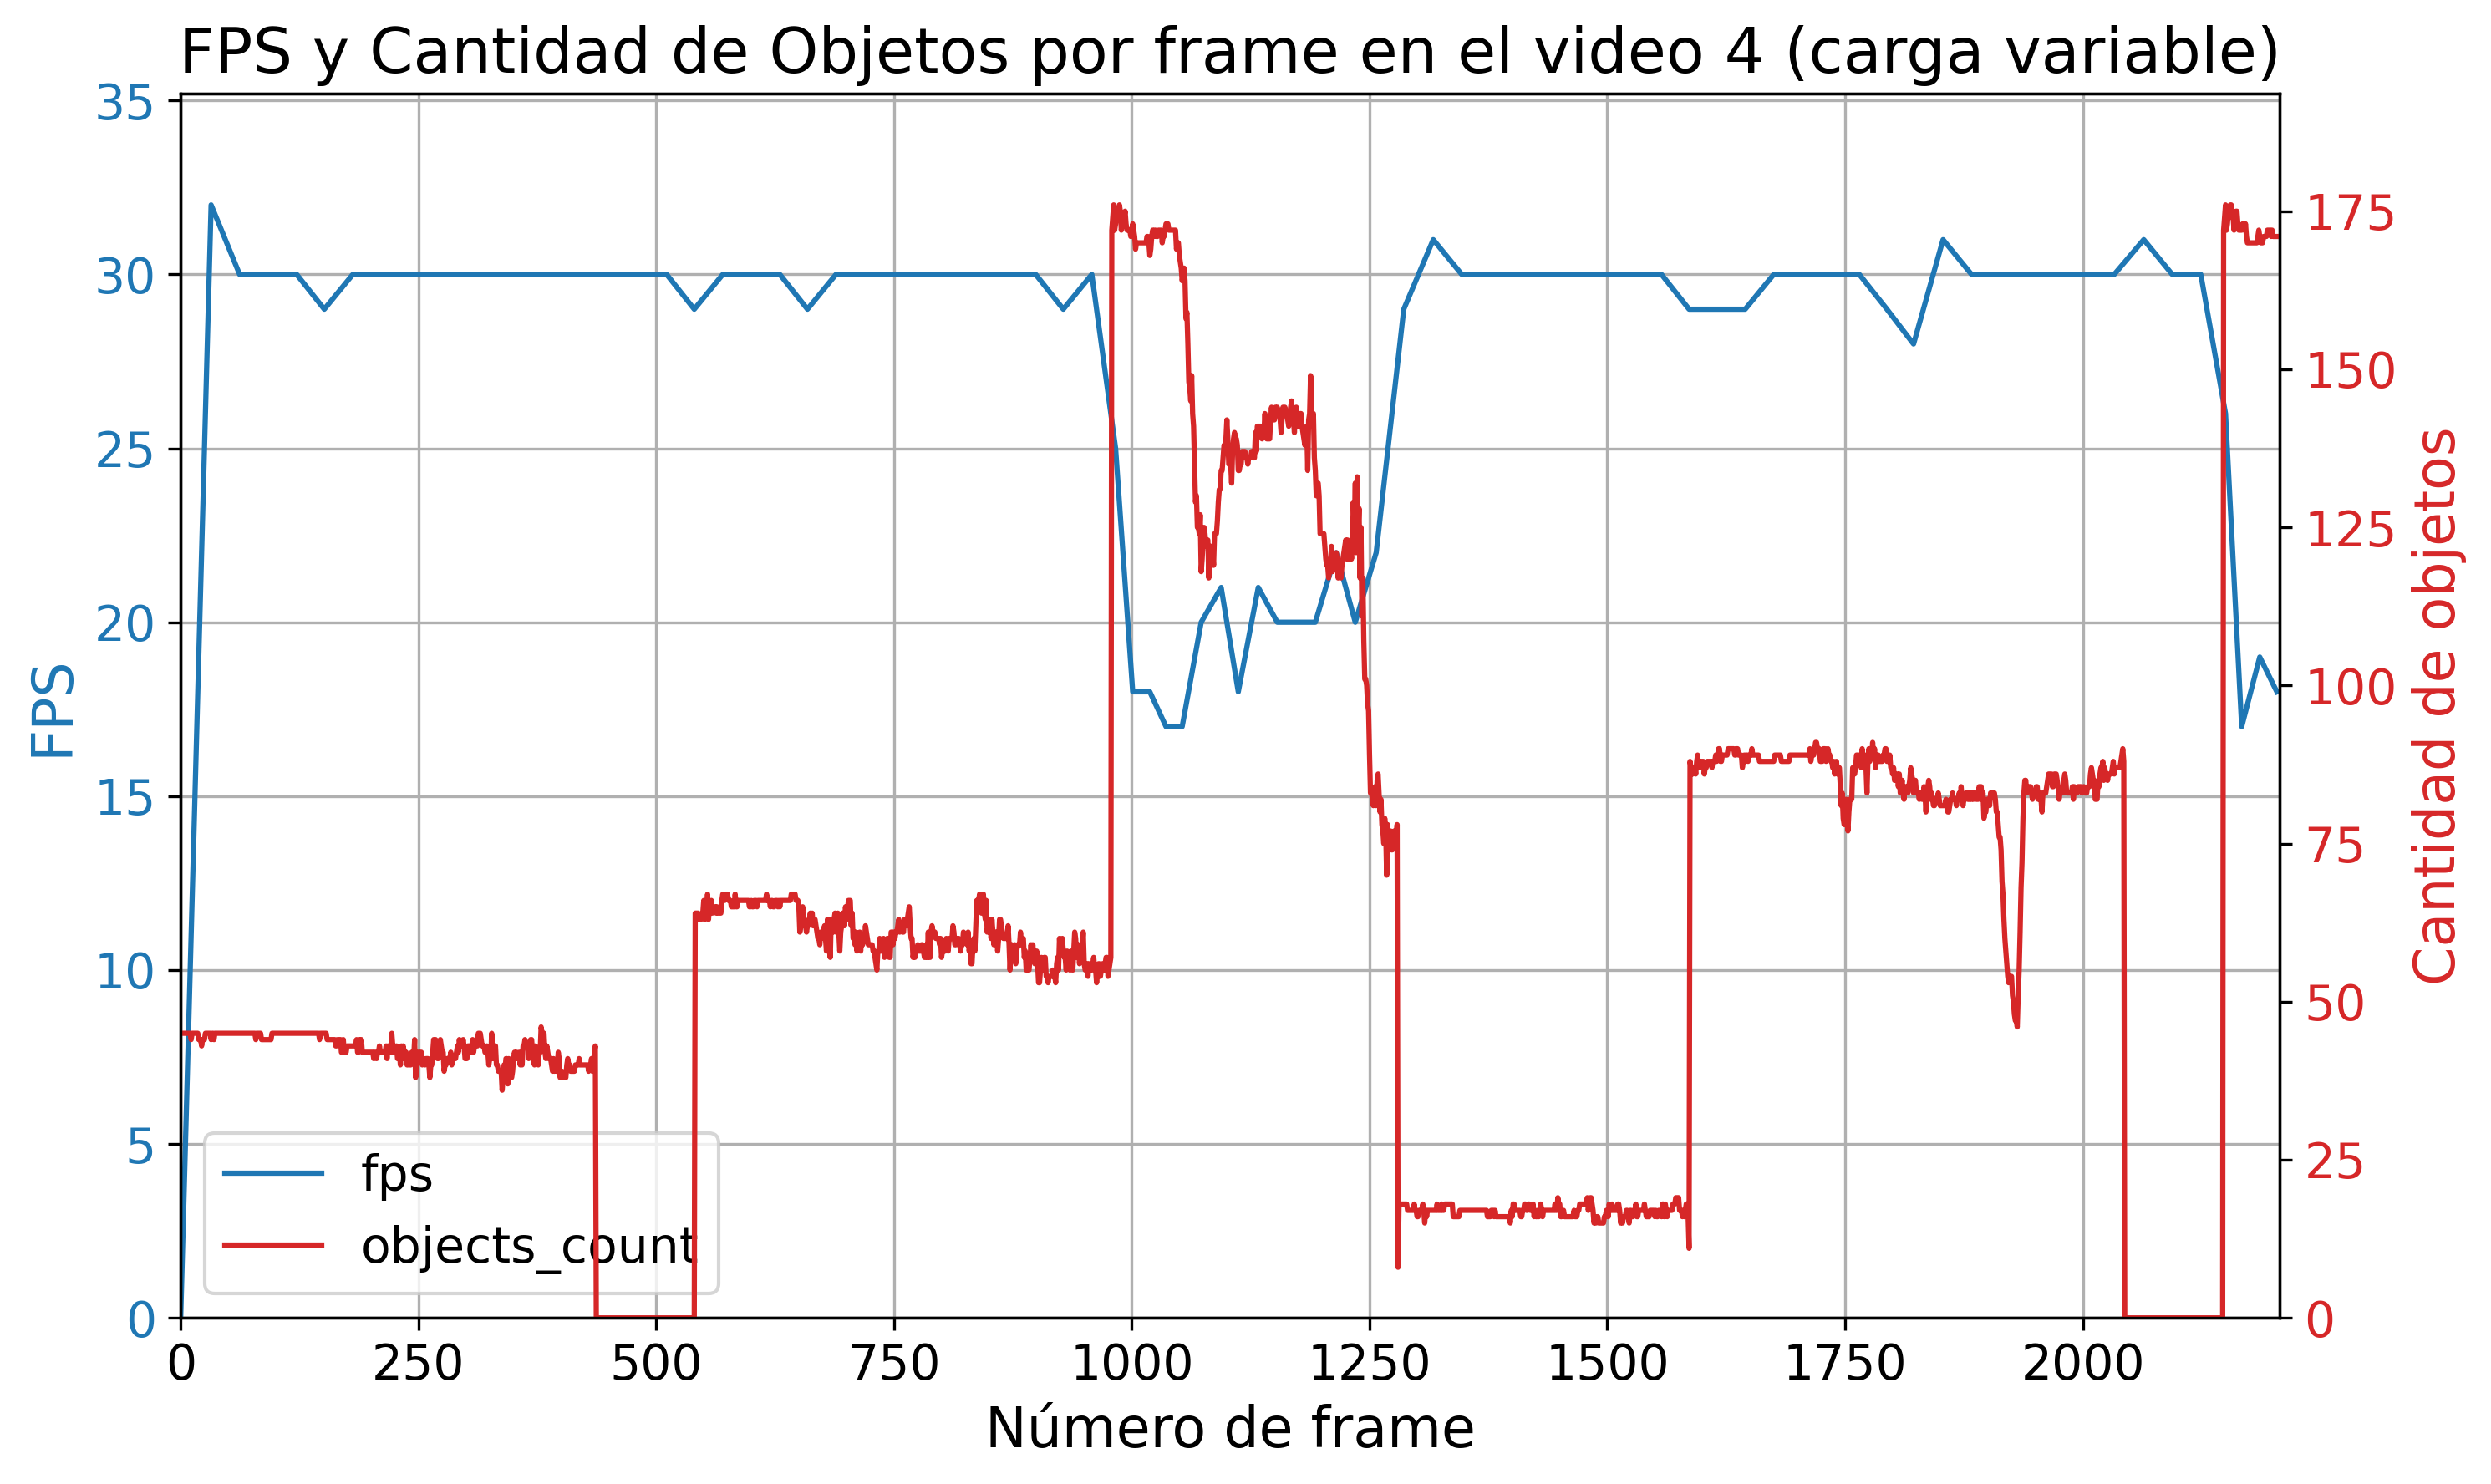
\includegraphics[width=0.8\textwidth]{excels/inferencia/cantidad_objetos/resultados/variable_fps_vs_object_count/fps_vs_object_count.png}
   \caption{FPS y cantidad de objetos en función del tiempo para el vídeo de carga variable.}
   \label{fig:fps_vs_object_count}
\end{figure}

El análisis de la Tabla \ref{tab:experimento_objetos} también refleja una clara correlación inversa entre la cantidad de objetos y la eficiencia energética del sistema, expresada en fotogramas por vatio (Frames/W). A mayor densidad de objetos, menor es esta eficiencia, lo que indica que el sistema requiere proporcionalmente más energía para procesar escenas complejas. Este comportamiento se alinea con la expectativa de que una mayor carga de trabajo implica un incremento en el consumo de recursos computacionales y energéticos. Esta tendencia se confirma al examinar los niveles de utilización de hardware: el aumento en la cantidad de objetos se corresponde directamente con una mayor utilización media de CPU evidenciando el incremento gradual en la demanda de recursos del sistema conforme crece la complejidad de la escena analizada.



\begin{figure}[H]
   \centering
   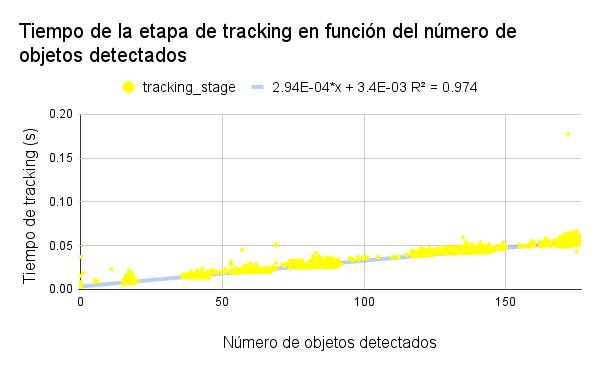
\includegraphics[width=0.8\textwidth]{images/analisis_de_la_solucion/cantidad_objetos/tiempo_etapa_tracking_cantidad_objetos.png}
   \caption{Tiempo de ejecución de la etapa de seguimiento en función de la cantidad de objetos.}
   \label{fig:tiempo_etapa_tracking_cantidad_objetos}
\end{figure}

Con los datos obtenidos, se ha creado una gráfica que muestra el tiempo de ejecución de la etapa de seguimiento en función de la cantidad de objetos presentes en el flujo de vídeo. La Figura \ref{fig:tiempo_etapa_tracking_cantidad_objetos} ilustra la relación empírica que describe esta dependencia. Mediante un análisis de regresión lineal, se ha obtenido la siguiente ecuación:

\begin{equation}
t_{seguimiento} = 2.94 \times 10^{-4} \times n_{objetos} + 3.4 \times 10^{-3}
\end{equation}

donde $t_{seguimiento}$ es el tiempo de ejecución de la etapa de seguimiento en segundos y $n_{objetos}$ es la cantidad de objetos. Esta fórmula presenta un coeficiente de determinación (R²) de 0.974, lo que indica un ajuste excelente al comportamiento observado.

Para determinar el umbral teórico donde el sistema dejaría de cumplir los requisitos de tiempo real (33.3 ms por fotograma), podemos despejar $n_{objetos}$ de la ecuación anterior:

\begin{align}
   2.94 \times 10^{-4} \times n_{objetos} + 3.4 \times 10^{-3} &\leq 33.3 \times 10^{-3} \\
   2.94 \times 10^{-4} \times n_{objetos} &\leq 33.3 \times 10^{-3} - 3.4 \times 10^{-3} \\
   2.94 \times 10^{-4} \times n_{objetos} &\leq 29.9 \times 10^{-3} \\
   n_{objetos} &\leq \frac{29.9 \times 10^{-3}}{2.94 \times 10^{-4}} \\
   n_{objetos} &\leq 101.70
\end{align}

Este cálculo teórico revela que el sistema alcanzaría su límite de procesamiento en tiempo real aproximadamente con 102 objetos, lo que coincide notablemente con los resultados experimentales mostrados en la Figura \ref{fig:fps_vs_object_count}, donde se observaba una degradación significativa del rendimiento alrededor de los 100 objetos.

\begin{figure}[H]
   \centering
   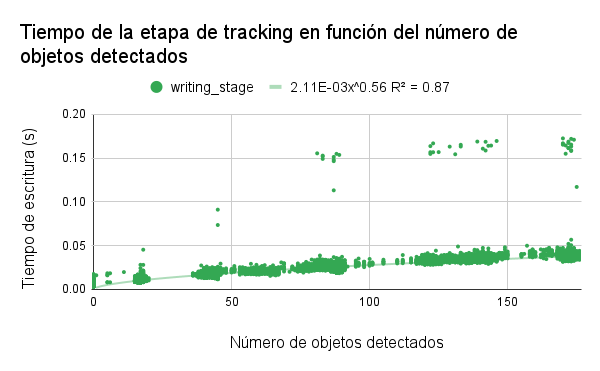
\includegraphics[width=0.8\textwidth]{images/analisis_de_la_solucion/cantidad_objetos/tiempo_etapa_escritura_cantidad_objetos.png}
   \caption{Tiempo de ejecución de la etapa de escritura en función de la cantidad de objetos.}
   \label{fig:tiempo_etapa_escritura_cantidad_objetos}
\end{figure}

Con los datos obtenidos, se ha creado una gráfica que muestra el tiempo de ejecución de la etapa de escritura en función de la cantidad de objetos presentes en el flujo de vídeo. La Figura \ref{fig:tiempo_etapa_escritura_cantidad_objetos} ilustra la relación empírica que describe esta dependencia. Mediante un análisis de regresión polinómica, se ha obtenido la siguiente ecuación:

\begin{equation}
   t_{escritura} = 2.11 \times 10^{-3} \times n_{objetos}^{0.56}
\end{equation}
donde $t_{escritura}$ es el tiempo de ejecución de la etapa de escritura en segundos y $n_{objetos}$ es la cantidad de objetos. Esta fórmula presenta un coeficiente de determinación (R²) de 0.874, lo que indica un ajuste aceptable al comportamiento observado.
Para determinar el umbral teórico donde el sistema dejaría de cumplir los requisitos de tiempo real (33.3 ms por fotograma), podemos despejar $n_{objetos}$ de la ecuación anterior:
\begin{align}
   2.11 \times 10^{-3} \times n_{objetos}^{0.56} &\leq 33.3 \times 10^{-3} \\
   n_{objetos}^{0.56} &\leq \frac{33.3 \times 10^{-3}}{2.11 \times 10^{-3}} \\
   n_{objetos} &\leq \left(\frac{33.3}{2.11}\right)^{\frac{1}{0.56}} \\
   n_{objetos} &\leq 137.90
\end{align}

Este cálculo teórico revela que el sistema alcanzaría su límite de procesamiento en tiempo real para la etapa de escritura aproximadamente con 138 objetos. No obstante, y aunque puedan existir algunos valores atípicos (\textit{outliers}), la etapa de seguimiento (\textit{tracking}) es la que marcará el cuello de botella del sistema frente a la de escritura.

Como conclusiones, se puede afirmar que el rendimiento del sistema es altamente sensible a la cantidad de objetos presentes en el flujo de vídeo. El umbral de aproximadamente 100 objetos constituye un límite crítico, donde la etapa de seguimiento comienza a experimentar un aumento significativo en su tiempo de ejecución, haciendo que el sistema no pueda cumplir con los requisitos de tiempo real.

\section{Tipo de segmentación} \label{sub:analisis_segmentacion}
Como se ha comentado en la sección \ref{sec:segmentacion_etapas}, el sistema se puede segmentar de diferentes maneras. En esta sección se analizará el rendimiento de la solución propuesta variando el tipo de segmentación.

Repasando la sección \ref{sec:segmentacion_etapas}, se han implementado cinco tipos de modos de segmentación:
\begin{enumerate}
   \item \textbf{Ejecución secuencial} (subsección \ref{sub:secuencial}): Cada etapa del sistema se ejecuta de forma consecutiva. Este es el enfoque base y no se considera una segmentación propiamente dicha, sino el punto de partida para la comparación.
   \item \textbf{Segmentación por hilos} (subsección \ref{sub:segmentacion_hilos}): Cada etapa del sistema se ejecuta en un hilo independiente.
   \item \textbf{Segmentación por procesos} (subsección \ref{sub:segmentacion_procesos}): Cada etapa del sistema se ejecuta en un proceso independiente.
   \item \textbf{Segmentación por hardware} (subsección \ref{sub:segmentacion_hardware}): La etapa de inferencia se descarga a los aceleradores de hardware (GPU o DLA).
   \item \textbf{Segmentación por procesos con memoria compartida} (subsección \ref{sub:segmentacion_memoria_compartida}): Cada etapa del sistema se ejecuta en un proceso independiente y se comunica mediante memoria compartida.
\end{enumerate}

Para evaluar el rendimiento de cada tipo de segmentación, se han realizado pruebas utilizando el vídeo de 84 objetos (carga alta y constante) como entrada estándar. Este vídeo presenta una carga computacional significativa, lo que permite observar las diferencias de rendimiento entre los distintos tipos de segmentación. Para todas las pruebas se ha utilizado el modelo de detección de objetos YOLO11n, optimizado mediante NVIDIA TensorRT para su ejecución en la GPU. Se configuró para operar con precisión FP16 y con el perfil de energía del dispositivo Jetson ajustado al modo de máxima potencia (MAXN). 


Primero se va analizar el rendimiento de cada tipo de segmentación utilizando la metodología de ejecución a máxima capacidad, donde los fotogramas se entregan al sistema consecutivamente, tan pronto como el procesamiento del fotograma anterior ha concluido, utilizando colas intermedias que no descartan fotogramas. En este escenario, se mide el tiempo total que el sistema tarda en procesar la secuencia completa, lo que permite evaluar su rendimiento máximo (throughput) y compararlo con la duración real del vídeo.

\begin{table}[H]
   \centering
   \resizebox{\textwidth}{!}{% Ajusta al ancho de página
   \pgfplotstabletypeset[
       col sep=comma,
       header=true,
       columns={modo_segmentacion,frames_procesados,tiempo_ejecucion_s,FPS,LFPS,potencia_media_consumida_W,energia_consumida_J,frames_por_W,speedup,avg_GPU,avg_CPU},
       display columns/0/.style={column name=Modo de Segmentación, column type={c}, string type},
       display columns/1/.style={column name=Frames Procesados, column type={c}, fixed, precision=0},
       display columns/2/.style={column name=Tiempo Ejec. (s), column type={c}, fixed, precision=2},
       display columns/3/.style={column name=FPS, column type={c}, fixed, precision=2},
       display columns/4/.style={column name=LFPS, column type={c}, fixed, precision=2},
       display columns/5/.style={column name=Potencia media (W), column type={c}},
       display columns/6/.style={column name=Energía (J), column type={c}},
       display columns/7/.style={column name=Frames/W, column type={c}, fixed, precision=2},
       display columns/8/.style={column name=Speedup, column type={c}, fixed, precision=2},
       display columns/9/.style={column name=GPU Avg. \protect\footnotemark, column type={c}},
       display columns/10/.style={column name=CPU Avg., column type={c}},
       every head row/.style={before row=\toprule, after row=\midrule},
       every last row/.style={after row=\bottomrule},
       empty cells with={NaN}
   ]{excels/inferencia/modo_segmentacion/datos/max_fps.csv}
   }
   \caption{Resultados del experimento con distintos tipos de segmentación a máxima capacidad.}
   \label{tab:experimento_segmentacion_max_fps}
\end{table}


\footnotetext{\footnotesize En la configuración de segmentación por hardware, se utilizan la GPU y los dos núcleos DLA; sin embargo, solo se muestra la utilización de la GPU, ya que la herramienta de monitorización de NVIDIA no reporta la utilización media de la DLA.}

A partir de los datos de la Tabla \ref{tab:experimento_segmentacion_max_fps}, se pueden extraer las siguientes conclusiones sobre el rendimiento de los diferentes enfoques de segmentación:

La ejecución secuencial, como era de esperar, ofrece el rendimiento más bajo, sirviendo como línea base para las comparaciones de speedup. Al no solapar ninguna operación, su capacidad de procesamiento es la más limitada.

La segmentación por hilos es la que ofrece el peor rendimiento después de la secuencial. Esto se debe fundamentalmente al Global Interpreter Lock (GIL) de Python, que impide el paralelismo real entre hilos dentro de un mismo proceso, limitando la capacidad de aprovechar múltiples núcleos de CPU.

La segmentación por procesos mejora esta situación al introducir paralelismo real, ya que cada proceso tiene su propio intérprete Python y, por ende, su propio GIL. Sin embargo, la comunicación estándar entre procesos mediante colas introduce una sobrecarga que impide extraer el máximo rendimiento.

La segmentación basada en hardware, que asigna la inferencia a la GPU o DLA, ofrece un rendimiento notable y es capaz de procesar el vídeo en tiempo real. Si bien su velocidad podría ser comparable a la segmentación por procesos con memoria compartida, su consumo energético es superior debido al uso simultáneo de la GPU y, en su caso, la DLA. El rendimiento se ve limitado porque el modelo no se ejecuta en su totalidad en la DLA, lo que resulta en que una porción de la carga de trabajo recaiga sobre la GPU. Esto impide que las unidades de procesamiento operen de forma completamente independiente, generando competencia por los recursos de la GPU.

Finalmente, la segmentación por procesos con memoria compartida es la que ofrece el mejor rendimiento global. Este enfoque combina el paralelismo real de los procesos con una comunicación entre ellos mucho más eficiente gracias al uso de memoria compartida, lo que minimiza la sobrecarga de la transferencia de datos. Esta combinación la posiciona como la opción más rápida, siendo también capaz de procesar el vídeo en tiempo real (30 fps).

Ahora se va a analizar el rendimiento de cada tipo de segmentación utilizando la metodología de ejecución en tiempo real, donde el sistema debe procesar cada fotograma en un tiempo máximo de 33.3 ms (30 fps). Si no logra hacerlo, el fotograma se descarta. Esta metodología permite evaluar la capacidad del sistema para operar en tiempo real y medir la tasa de fotogramas perdidos (LFPS).


\begin{table}[H]
   \centering
   \resizebox{\textwidth}{!}{% Ajusta al ancho de página
   \pgfplotstabletypeset[
       col sep=comma,
       header=true,
       columns={modo_segmentacion,frames_procesados,tiempo_ejecucion_s,FPS,LFPS,potencia_media_consumida_W,energia_consumida_J,frames_por_W,avg_GPU,avg_CPU},
       display columns/0/.style={column name=Modo de Segmentación, column type={c}, string type},
       display columns/1/.style={column name=Frames Procesados, column type={c}, fixed, precision=0},
       display columns/2/.style={column name=Tiempo Ejec. (s), column type={c}, fixed, precision=2},
       display columns/3/.style={column name=FPS, column type={c}, fixed, precision=2},
       display columns/4/.style={column name=LFPS, column type={c}, fixed, precision=2},
       display columns/5/.style={column name=Potencia media (W), column type={c}},
       display columns/6/.style={column name=Energía (J), column type={c}},
       display columns/7/.style={column name=Frames/W, column type={c}, fixed, precision=2},
       display columns/8/.style={column name=GPU Avg., column type={c}},
       display columns/9/.style={column name=CPU Avg., column type={c}},
       every head row/.style={before row=\toprule, after row=\midrule},
       every last row/.style={after row=\bottomrule},
       empty cells with={NaN}
   ]{excels/inferencia/modo_segmentacion/datos/30_fps.csv}
   }
   \caption{Resultados del experimento con distintos tipos de segmentación a 30 fps.}
   \label{tab:experimento_segmentacion_30_fps}
\end{table}

Como se puede observar en la Tabla \ref{tab:experimento_segmentacion_30_fps}, el tipo de segmentación influye significativamente en el rendimiento del sistema. La ejecución secuencial es inviable para tiempo real, presentando la tasa más alta de fotogramas perdidos (LFPS) con 19.87 fps. La segmentación por hilos, aunque mejora ligeramente, sigue siendo inviable para tiempo real, con una LFPS de 11.51, lo que confirma los resultados de la ejecución a máxima capacidad. Aunque la segmentación por procesos mejora este valor a 7.29 LFPS, tampoco alcanza los requisitos de tiempo real. Por su parte, la segmentación basada en hardware logra operar en tiempo real, pero a costa de un mayor consumo energético. Finalmente, la segmentación por procesos con memoria compartida destaca como la opción más eficiente, logrando el mejor rendimiento en tiempo real (LFPS de 0.91) con el menor consumo energético.

Como conclusión, la segmentación por procesos con memoria compartida es la más adecuada para aplicaciones en tiempo real, ya que combina un rendimiento óptimo con un consumo energético eficiente. Este enfoque permite al sistema operar de manera efectiva bajo condiciones de alta carga computacional, cumpliendo con los requisitos de tiempo real sin comprometer la eficiencia energética.

\section{Modelo y talla} \label{sub:modelo_talla}
En esta sección se analizará el rendimiento de la solución propuesta variando el modelo de detección de objetos y sus diferentes tallas.

Repasando la tabla \ref{tab:yolo_all_variants_comparison}, se han empleado tres modelos de detección de objetos: YOLOv5, YOLOv8 y YOLO11. Cada uno de estos modelos tiene diferentes tallas, que son versiones optimizadas para diferentes capacidades computacionales. 

Para la evaluación del rendimiento de cada modelo y sus diferentes tallas, se estableció una configuración base común: los modelos de detección de objetos se optimizaron con NVIDIA TensorRT para su ejecución en la GPU, utilizando precisión FP16 y el perfil de energía MAXN del dispositivo Jetson AGX Xavier. Adicionalmente, se empleó la segmentación por procesos con memoria compartida, identificada en análisis previos como la más eficiente en rendimiento y consumo energético. Sobre esta configuración, las pruebas se realizaron utilizando como entrada estándar el vídeo de 84 objetos (carga alta y constante), lo que permite someter al sistema a una carga computacional elevada y así comparar objetivamente las distintas variantes de modelos y tallas.

\begin{table}[H]
   \centering
   \resizebox{\textwidth}{!}{% Ajusta al ancho de página
   \pgfplotstabletypeset[
       col sep=comma,
       header=true,
       columns={modelo,frames_procesados,Tejecucion_s,FPS,LFPS,potencia_media_consumida_W,energia_consumida_J,Frames_W,Average_GPU,Average_CPU,Tpreprocesado_ms,Tinferencia_ms,Tpostprocesado_ms},
       display columns/0/.style={column name=Modelo, column type={c}, string type},
       display columns/1/.style={column name=Frames Procesados, column type={c}, fixed, precision=0},
       display columns/2/.style={column name=Tiempo Ejec. (s), column type={c}, fixed, precision=2},
       display columns/3/.style={column name=FPS, column type={c}, fixed, precision=2},
       display columns/4/.style={column name=LFPS, column type={c}, fixed, precision=2},
       display columns/5/.style={column name=Potencia media (W), column type={c}, fixed, precision=3},
       display columns/6/.style={column name=Energía (J), column type={c}, fixed, precision=2},
       display columns/7/.style={column name=Frames/W, column type={c}, fixed, precision=2},
       display columns/8/.style={column name=GPU Avg. (\%), column type={c}, fixed, precision=2},
       display columns/9/.style={column name=CPU Avg. (\%), column type={c}, fixed, precision=2},
       display columns/10/.style={column name=T. Prepro. (ms), column type={c}, fixed, precision=2},
       display columns/11/.style={column name=T. Infer. (ms), column type={c}, fixed, precision=2},
       display columns/12/.style={column name=T. Postpro. (ms), column type={c}, fixed, precision=2},
       every head row/.style={before row=\toprule, after row=\midrule},
       every last row/.style={after row=\bottomrule},
       empty cells with={NaN}
   ]{excels/inferencia/modelo_talla/data/max_fps.csv}
   }
   \caption{Resultados del experimento con distintos modelos y tallas a máxima capacidad con un vídeo de carga alta y constante.}
   \label{tab:experimento_modelo_talla_max_fps_carga_alta_constante}
\end{table}

Al analizar los resultados presentados en la Tabla \ref{tab:experimento_modelo_talla_max_fps_carga_alta_constante}, se observa una notable similitud en el rendimiento de fotogramas por segundo (FPS) entre todos los modelos y sus respectivas tallas, manteniéndose en un rango aproximado de 28 ± 1 FPS. Esta homogeneidad en la velocidad de procesamiento se explica por la naturaleza del vídeo de prueba utilizado, que presenta una carga alta y constante de objetos. En este escenario, el rendimiento global del sistema se ve limitado predominantemente por la capacidad de las etapas posteriores a la inferencia (como el seguimiento y la escritura) para procesar la gran cantidad de objetos detectados, más que por la complejidad intrínseca o la velocidad de la etapa de inferencia en sí misma. Esto enmascara las diferencias potenciales en la velocidad de inferencia pura que podrían observarse bajo condiciones de menor carga de objetos.

No obstante, al considerar la eficiencia energética, medida en fotogramas por vatio (Frames/W), emergen diferencias significativas. Los modelos YOLO11n y YOLOv8n se destacan como las opciones más eficientes, logrando un mayor número de fotogramas procesados por cada vatio de energía consumida. En contraste, el modelo YOLO11l, a pesar de ofrecer una tasa de FPS comparable, presenta un consumo energético superior, lo que resulta en una menor eficiencia. Esta diferencia se atribuye al mayor número de parámetros del modelo YOLO11l, que inherentemente demanda más recursos computacionales y, por ende, energéticos para su ejecución.


\begin{figure}[H]
   \centering
   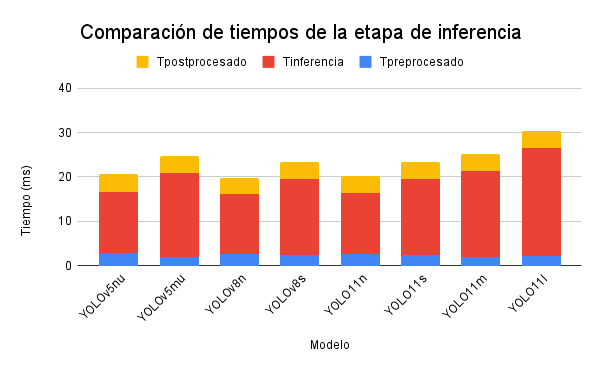
\includegraphics[width=0.7\textwidth]{images/analisis_de_la_solucion/modelo_talla/tiempos_inferencia.png}
   \caption{Tiempos de ejecución de la etapa de inferencia para los diferentes modelos y tallas.}
   \label{fig:tiempos_inferencia}
\end{figure}
Un análisis detallado de los tiempos de la etapa de inferencia, presentado en la Figura \ref{fig:tiempos_inferencia}, revela que los modelos YOLOv8n y YOLO11n destacan por su menor tiempo de ejecución. En contraste, YOLOv5mu y YOLO11l exhiben tiempos más elevados, una tendencia que se alinea con el mayor consumo energético reportado en la Tabla \ref{tab:experimento_modelo_talla_max_fps_carga_alta_constante}.

Ahora se va a analizar el rendimiento de cada modelo y sus diferentes tallas utilizando la metodología de ejecución en tiempo real, donde el sistema debe procesar cada fotograma en un tiempo máximo de 33.3 ms (30 fps). Si no logra hacerlo, el fotograma se descarta. Esta metodología permite evaluar la capacidad del sistema para operar en tiempo real y medir la tasa de fotogramas perdidos (LFPS).

\begin{table}[H]
   \centering
   \resizebox{\textwidth}{!}{% Ajusta al ancho de página
   \pgfplotstabletypeset[
       col sep=comma,
       header=true,
       columns={modelo,frames_procesados,Tejecucion_s,FPS,LFPS,potencia_media_consumida_W,energia_consumida_J,Frames_W,mAP50_95},
       display columns/0/.style={column name=Modelo, column type={c}, string type},
       display columns/1/.style={column name=Frames Procesados, column type={c}, fixed, precision=0},
       display columns/2/.style={column name=Tiempo Ejec. (s), column type={c}, fixed, precision=2},
       display columns/3/.style={column name=FPS, column type={c}, fixed, precision=2},
       display columns/4/.style={column name=LFPS, column type={c}, fixed, precision=2},
       display columns/5/.style={column name=Potencia media (W), column type={c}, fixed, precision=3},
       display columns/6/.style={column name=Energía (J), column type={c}, fixed, precision=2},
       display columns/7/.style={column name=Frames/W, column type={c}, fixed, precision=2},
      %  display columns/8/.style={column name={GPU Avg. (\%)}, column type={c}, fixed, precision=2},
      %  display columns/9/.style={column name={CPU Avg. (\%)}, column type={c}, fixed, precision=2},
      %  display columns/10/.style={column name=T. Prepro. (ms), column type={c}, fixed, precision=2},
      %  display columns/11/.style={column name=T. Infer. (ms), column type={c}, fixed, precision=2},
      %  display columns/12/.style={column name=T. Postpro. (ms), column type={c}, fixed, precision=2},
       display columns/8/.style={column name={mAP$_{50-95}$}, column type={c}, fixed, precision=2},
       every head row/.style={before row=\toprule, after row=\midrule},
       every last row/.style={after row=\bottomrule},
       empty cells with={NaN}
   ]{excels/inferencia/modelo_talla/data/30_fps.csv}
   }
   \caption{Resultados del experimento con distintos modelos y tallas a 30 fps.}
   \label{tab:experimento_modelo_talla_30_fps}
\end{table}

Los resultados de la Tabla \ref{tab:experimento_modelo_talla_30_fps} muestran una tendencia general similar a la observada en la Tabla \ref{tab:experimento_modelo_talla_max_fps_carga_alta_constante} en términos de rendimiento.
Sin embargo, la Tabla \ref{tab:experimento_modelo_talla_30_fps} permite un análisis más detallado de la tasa de fotogramas perdidos (LFPS) para cada combinación de modelo y talla.
Se observa que el modelo YOLOv8s presenta la tasa de LFPS más alta, alcanzando 2.39 LFPS.
A pesar de esto, todas las variantes de modelos y tallas evaluadas mantienen una tasa de LFPS que podría considerarse aceptable para un sistema de visión artificial operando en tiempo real a 30 fps, ya que el sistema podría continuar funcionando de manera efectiva.
El modelo YOLOv8n registra la tasa de LFPS más baja (1.2 LFPS), aunque las diferencias entre los modelos no son drásticas en este aspecto.

Para seleccionar el modelo y la talla más adecuados, es crucial considerar un equilibrio entre el consumo energético y la precisión del modelo. En el contexto de la tarea actual, que consiste en clasificar canicas de diferentes colores y con/sin defectos, la complejidad es relativamente baja.
Como resultado, todos los modelos y tallas evaluados alcanzan niveles de precisión (mAP50-95) similares, tal como se evidencia en la última columna de la Tabla \ref{tab:experimento_modelo_talla_30_fps}.
Dada esta similitud en precisión, para esta aplicación específica, se podría priorizar la elección del modelo y talla que ofrezca el menor consumo energético.
No obstante, en aplicaciones donde la precisión de detección sea un factor crítico, la selección debería inclinarse hacia el modelo y talla que demuestre el mayor rendimiento en dicha métrica, incluso si esto implica un mayor consumo energético.



\section{Precisión Numérica y Acelerador de Inferencia} \label{sub:precision_numerica_dispositivo}
En esta sección se analizará el rendimiento de la solución propuesta variando la precisión numérica (FP32, FP16, INT8) del modelo de detección de objetos y el acelerador de inferencia (CPU, GPU, DLA).

Para la realización de estas pruebas, se ha utilizado el modelo YOLO11n. Para la ejecución en GPU y DLA, el modelo fue optimizado con NVIDIA TensorRT, evaluándose las precisiones FP32, FP16 e INT8. En el caso de la ejecución en CPU, se empleó el modelo YOLO11n sin la optimización de TensorRT, ya que esta no es aplicable a dicho dispositivo. La exportación del modelo de PyTorch a TensorRT con precisión INT8 requiere un conjunto de datos de calibración; para este propósito, se utilizó un subconjunto de 100 imágenes extraídas del conjunto de entrenamiento original, con el fin de calibrar el modelo y optimizar su rendimiento para la inferencia en INT8. Por último, la precisión de validación de todos los modelos en la Tabla \ref{tab:experimento_precision_dispositivo_max_fps_carga_alta_constante} es casi idéntica, con un mAP50-95 de 0.77 para todas las variantes, lo que indica que la precisión del modelo no se ve afectada significativamente por la reducción de la precisión numérica posiblemente debido a la sencillez de la tarea de detección de objetos en este caso específico.


\begin{table}[H]
   \centering
   \resizebox{\textwidth}{!}{% Ajusta al ancho de página
   \pgfplotstabletypeset[
       col sep=comma,
       header=true,
       columns={Dispositivo,Precision,frames_procesados,tejecucion,FPS,LFPS,potencia_media_consumida,energia_consumida,Frames/W,Average_GPU,Average_CPU,mAP50-95},
      display columns/0/.style={column name=Acelerador, column type={c}, string type},
      display columns/1/.style={column name=Precisión, column type={c}, string type},
      display columns/2/.style={column name=Frames Procesados, column type={c}, fixed, precision=0},
      display columns/3/.style={column name=Tiempo Ejec. (s), column type={c}, fixed, precision=2},
      display columns/4/.style={column name=FPS, column type={c}, fixed, precision=2},
      display columns/5/.style={column name=LFPS, column type={c}, fixed, precision=2},
      display columns/6/.style={column name=Potencia media (W), column type={c}, fixed, precision=3},
      display columns/7/.style={column name=Energía (J), column type={c}, fixed, precision=2},
      display columns/8/.style={column name=Frames/W, column type={c}, fixed, precision=2},
      display columns/9/.style={column name=GPU Avg. (\%), column type={c}, fixed, precision=2},
      display columns/10/.style={column name=CPU Avg. (\%), column type={c}, fixed, precision=2},
      display columns/11/.style={column name={mAP$_{50-95}$}, column type={c}, fixed, precision=4},
       every head row/.style={before row=\toprule, after row=\midrule},
       every last row/.style={after row=\bottomrule},
       empty cells with={NaN}
   ]{excels/inferencia/precision_device/data/max_fps.csv}
   }
   \caption{Resultados del experimento con distintos modelos y tallas a máxima capacidad con un vídeo de carga alta y constante.}
   \label{tab:experimento_precision_dispositivo_max_fps_carga_alta_constante}
\end{table}

Basándose en los resultados de la Tabla \ref{tab:experimento_precision_dispositivo_max_fps_carga_alta_constante}, se pueden extraer varias conclusiones sobre el impacto de la precisión numérica y el acelerador de inferencia.

En primer lugar, la ejecución del modelo en CPU resulta completamente inviable para aplicaciones en tiempo real. Como se aprecia en la tabla, la tasa de procesamiento es de tan solo 0.93 FPS, lo que demuestra la necesidad de aceleradores hardware para esta tarea.

Al comparar el rendimiento de la GPU y los Deep Learning Accelerators (DLA), se observa que la DLA, en teoría diseñada para manejar cargas de trabajo específicas de inferencia de manera eficiente (como se repasó en la sección \ref{sec:jetson}), ofrece un rendimiento similar al de la GPU en este caso. Sin embargo, es crucial señalar que el modelo YOLO11n, tanto en precisión FP16 como en INT8, no se ejecuta completamente en la DLA, ya que algunas de sus operaciones no son compatibles con este dispositivo. Esto implica que la GPU también participa en el procesamiento. Este fenómeno se hace particularmente evidente en la precisión INT8, donde ninguna capa del modelo se ejecuta en la DLA, recayendo toda la carga en la GPU.
\begin{figure}[H]
   \centering
   \includegraphics[width=0.85\textwidth]{images/analisis_de_la_solucion/precision_device/exportación_FP16_DLA.png}
   \caption{Exportación del modelo YOLO11n con TensorRT a FP16 para su ejecución en la DLA.}
   \label{fig:exportacion_FP16_DLA}
\end{figure}
En la precisión FP16, como se ilustra en la Figura \ref{fig:exportacion_FP16_DLA}, la DLA se encarga de 6 de las 34 operaciones/capas del modelo, mientras que la GPU procesa las 28 restantes. En esencia, la DLA no logra descargar completamente a la GPU, lo que limita su capacidad para operar de forma independiente y optimizar el rendimiento general del sistema. Si bien en modelos más simples la DLA podría asumir una mayor proporción de las operaciones, la complejidad del modelo YOLO11n (y de forma similar para YOLOv5 y YOLOv8) impide que la DLA asuma una carga de trabajo más significativa.

Considerando la ejecución en GPU, la optimización con TensorRT, incluso manteniendo la precisión FP32, produce una notable aceleración en comparación con la ejecución del modelo sin optimizar en GPU. El modelo optimizado para GPU con TensorRT en FP32 alcanza un speedup de $\frac{183.29}{84.44} = 2.17\times$ frente a la GPU. Esto demuestra que TensorRT mejora drásticamente el rendimiento mediante optimizaciones como la fusión de capas y la eliminación de operaciones redundantes, resultando en una ejecución más eficiente.

En cuanto a las diferentes precisiones numéricas en la GPU (todas optimizadas con TensorRT), los resultados muestran un rendimiento en FPS similar entre FP32, FP16 e INT8.
\begin{figure}[H]
   \centering
   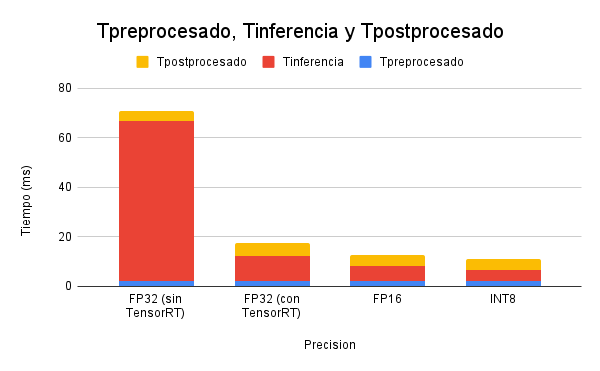
\includegraphics[width=0.7\textwidth]{images/analisis_de_la_solucion/precision_device/tiempos_inferencia_gpu.png}
   \caption{Tiempos de ejecución de la etapa de inferencia para las diferentes precisiones en GPU con TensorRT.}
   \label{fig:tiempos_inferencia_gpu}
\end{figure}
Un análisis más detallado de los tiempos de la etapa de inferencia, como se observa en la Figura \ref{fig:tiempos_inferencia_gpu}, revela una reducción en el tiempo de inferencia al utilizar precisiones más bajas. Aunque el impacto en los FPS totales del sistema es limitado por otros factores del \textit{pipeline} en este escenario de alta carga de objetos, es importante destacar que las precisiones FP16 e INT8 logran un menor consumo energético. Esto se debe a que estas precisiones reducidas requieren menos recursos computacionales, lo que se traduce en una mayor eficiencia energética. En particular, la precisión INT8 se presenta como la opción más eficiente en términos de consumo energético, alcanzando un rendimiento de 1.96 Frames/W.


\begin{table}[H]
   \centering
   \resizebox{\textwidth}{!}{% Ajusta al ancho de página
   \pgfplotstabletypeset[
      col sep=comma,
      header=true,
      columns={Dispositivo,Precision,frames_procesados,tejecucion,FPS,LFPS,potencia_media_consumida,energia_consumida,Frames/W,Average_GPU,Average_CPU,mAP50-95},
      display columns/0/.style={column name=Acelerador, column type={c}, string type},
      display columns/1/.style={column name=Precisión, column type={c}, string type},
      display columns/2/.style={column name=Frames Procesados, column type={c}, fixed, precision=0},
      display columns/3/.style={column name=Tiempo Ejec. (s), column type={c}, fixed, precision=2},
      display columns/4/.style={column name=FPS, column type={c}, fixed, precision=2},
      display columns/5/.style={column name=LFPS, column type={c}, fixed, precision=2},
      display columns/6/.style={column name=Potencia media (W), column type={c}, fixed, precision=3},
      display columns/7/.style={column name=Energía (J), column type={c}, fixed, precision=2},
      display columns/8/.style={column name=Frames/W, column type={c}, fixed, precision=2},
      display columns/9/.style={column name=GPU Avg. (\%), column type={c}, fixed, precision=2},
      display columns/10/.style={column name=CPU Avg. (\%), column type={c}, fixed, precision=2},
      display columns/11/.style={column name={mAP$_{50-95}$}, column type={c}, fixed, precision=4},
      every head row/.style={before row=\toprule, after row=\midrule},
      every last row/.style={after row=\bottomrule},
      empty cells with={NaN}
      ]{excels/inferencia/precision_device/data/30_fps.csv}
      }
      \caption{Resultados del experimento con distintos modelos y tallas a 30 fps con un vídeo de carga alta y constante.}
      \label{tab:experimento_precision_dispositivo_30_fps}
   \end{table}

   En la Tabla \ref{tab:experimento_precision_dispositivo_30_fps}, se observan las ejecuciones en tiempo real de los modelos con diferentes precisiones y dispositivos. Observando los resultados, como se ha mencionado anteriormente, la ejecución del modelo en CPU es completamente inviable para tiempo real, con una tasa de 0.79 FPS y 28.49 LFPS.

   En cuanto a la GPU, todas las precisiones (FP32, FP16 e INT8 con TensorRT) logran operar en tiempo real, con tasas de FPS de 28.42, 28.73 y 28.44 respectivamente, lo que indica que el sistema puede procesar los fotogramas a la velocidad requerida sin perder ninguno.

   La combinación de la GPU con la precisión INT8 es la más eficiente en términos de consumo energético, alcanzando 1.96 Frames/W.






   
   \section{Modo de energía y cores de la CPU} \label{sub:modo_energia}
   En esta sección, se analiza el impacto de la configuración energética del dispositivo NVIDIA Jetson AGX Xavier en el rendimiento del sistema. Se exploran distintos perfiles de energía predefinidos (10W, 15W, 30W y MAXN), los cuales ajustan tanto el número de núcleos de CPU activos como su frecuencia máxima de operación. El objetivo es evaluar cómo estas configuraciones influyen en la velocidad de procesamiento (FPS), el consumo energético y, por ende, la eficiencia energética global del sistema.

   Para la realización de estas pruebas, se ha utilizado el modelo YOLO11n con la precisión FP16 optimizado con TensorRT para su ejecución en la GPU, un video de 84 objetos (carga alta y constante) y la segmentación por procesos con memoria compartida.

\begin{table}[H]
   \centering
   \resizebox{\textwidth}{!}{% Ajusta al ancho de página
   \pgfplotstabletypeset[
      col sep=comma,
      header=true,
      columns={energy_mode,cpu_core,freq,processed_frame,execution_time,fps,lfps,average_power_consuption,energy_consuption,frames/w,average_gpu,average_cpu},
      display columns/0/.style={column name=Modo de Energía, column type={c}, string type},
      display columns/1/.style={column name=Núcleos de CPU, column type={c}, string type},
      display columns/2/.style={column name=Frecuencia (GHz), column type={c}, fixed, precision=2},
      display columns/3/.style={column name=Frames Procesados, column type={c}, fixed, precision=0},
      display columns/4/.style={column name=Tiempo Ejec. (s), column type={c}, fixed, precision=2},
      display columns/5/.style={column name=FPS, column type={c}, fixed, precision=2},
      display columns/6/.style={column name=LFPS, column type={c}, fixed, precision=2},
      display columns/7/.style={column name=Potencia media (W), column type={c}, fixed, precision=3},
      display columns/8/.style={column name=Energía (J), column type={c}, fixed, precision=2},
      display columns/9/.style={column name=Frames/W, column type={c}, fixed, precision=2},
      display columns/10/.style={column name=GPU Avg. (\%), column type={c}, fixed, precision=2},
      display columns/11/.style={column name=CPU Avg. (\%), column type={c}, fixed, precision=2},
      every head row/.style={before row=\toprule, after row=\midrule},
      every last row/.style={after row=\bottomrule},
      empty cells with={NaN}
      ]{excels/inferencia/modo_energia_cpu/data/max_fps.csv}
      }
      \caption{Resultados del experimento con distintos modelos y tallas a máxima capacidad con un vídeo de carga alta y constante.}
      \label{tab:experimento_modo_energia_cpu_max_fps_carga_alta_constante}
   \end{table}

   Observando los resultados de la Tabla \ref{tab:experimento_modo_energia_cpu_max_fps_carga_alta_constante}, se aprecia una clara influencia del perfil de energía y del número de núcleos de CPU activos en el rendimiento del sistema. En general, al aumentar el perfil de energía y la cantidad de núcleos habilitados, se observa una mejora en la tasa de fotogramas por segundo (FPS). Sin embargo, el perfil de energía de 30W presenta un comportamiento particular: la configuración óptima se alcanza con 4 núcleos de CPU. Esto se debe a que esta combinación ofrece la frecuencia máxima del procesador más alta (1.8 GHz) en comparación con las configuraciones de 6 y 8 núcleos bajo el mismo perfil (1.41 GHz y 1.2 GHz, respectivamente). Aunque la configuración de 30W con 4 núcleos exhibe el mayor consumo de potencia medio (9.535 W), resulta en el menor consumo de energía total (1136.27 J) debido a la reducción en el tiempo de ejecución en comparación con las configuraciones de 6 y 8 núcleos bajo el mismo perfil. Esto subraya la importancia de considerar tanto el consumo de potencia instantáneo como la duración total de la ejecución al evaluar la eficiencia energética del sistema.

   Para evaluar el rendimiento en condiciones de tiempo real, se utilizó el mismo vídeo de 84 objetos (carga alta y constante) y la segmentación por procesos con memoria compartida. Se estableció un límite de 33.3 ms por fotograma (30 FPS) para evaluar la capacidad del sistema para operar en tiempo real y medir la tasa de fotogramas perdidos (LFPS). Es importante señalar que, en los perfiles de energía más bajos, no se logró simular el tiempo real, lo que resultó en tiempos de ejecución superiores a los 80 segundos del vídeo a 30 FPS.

   \begin{table}[H]
      \centering
      \resizebox{\textwidth}{!}{% Ajusta al ancho de página
      \pgfplotstabletypeset[
         col sep=comma,
         header=true,
         columns={energy_mode,cpu_core,freq,processed_frame,execution_time,fps,lfps,average_power_consuption,energy_consuption,frames/w,average_gpu,average_cpu},
         display columns/0/.style={column name=Modo de Energía, column type={c}, string type},
         display columns/1/.style={column name=Núcleos de CPU, column type={c}, string type},
         display columns/2/.style={column name=Frecuencia (GHz), column type={c}, fixed, precision=2},
         display columns/3/.style={column name=Frames Procesados, column type={c}, fixed, precision=0},
         display columns/4/.style={column name=Tiempo Ejec. (s), column type={c}, fixed, precision=2},
         display columns/5/.style={column name=FPS, column type={c}, fixed, precision=2},
         display columns/6/.style={column name=LFPS, column type={c}, fixed, precision=2},
         display columns/7/.style={column name=Potencia media (W), column type={c}, fixed, precision=3},
         display columns/8/.style={column name=Energía (J), column type={c}, fixed, precision=2},
         display columns/9/.style={column name=Frames/W, column type={c}, fixed, precision=2},
         display columns/10/.style={column name=GPU Avg. (\%), column type={c}, fixed, precision=2},
         display columns/11/.style={column name=CPU Avg. (\%), column type={c}, fixed, precision=2},
         every head row/.style={before row=\toprule, after row=\midrule},
         every last row/.style={after row=\bottomrule},
         empty cells with={NaN}
         ]{excels/inferencia/modo_energia_cpu/data/30_fps.csv}
         }
         \caption{Resultados del experimento con distintos modelos y tallas a 30 fps con un vídeo de carga alta y constante.}
         \label{tab:experimento_modo_energia_cpu_30_fps}
      \end{table}

      La Tabla \ref{tab:experimento_modo_energia_cpu_30_fps} presenta los resultados de la simulación en tiempo real. Como se mencionó anteriormente, los perfiles de energía más bajos no lograron simular el tiempo real, evidenciado por tiempos de ejecución superiores a la duración del vídeo de prueba. De todos los perfiles de energía evaluados, únicamente la configuración de máximas prestaciones (MAXN) con 8 núcleos de CPU activos logró operar a una tasa de 26.69 FPS, lo que indica que el sistema puede procesar los fotogramas a una velocidad cercana a la requerida, aunque con cierta pérdida de fotogramas.



\section{Dispositivos Jetson} \label{sec:dispositivos_jetson}
En esta sección se analizará el rendimiento de la solución propuesta en diferentes dispositivos Jetson, específicamente en el Jetson Orin Nano, Jetson AGX Xavier  y Jetson AGX Orin. Se utilizará el modelo YOLO11n con la precisión FP16 optimizado con TensorRT para su ejecución en la GPU, un video de 84 objetos (carga alta y constante) y la segmentación por procesos con memoria compartida.

\chapter{Prueba de concepto} \label{chap:prueba_concepto}
Aqui se explicará la implementación de la solución propuesta en el entorno de producción con la cinta transportadora.

\section{Construcción del entorno} \label{sub:construccion_entorno}
Tras la fase de desarrollo y análisis de la solución propuesta, que se llevó a cabo utilizando vídeos pregrabados en un entorno de laboratorio, se procedió a la implementación de una prueba de concepto. Esta prueba simula un entorno de producción real mediante la construcción de una cinta transportadora sencilla. El principal objetivo de esta etapa es validar la viabilidad y el rendimiento de la solución en un escenario práctico, evaluando su capacidad para detectar y clasificar objetos (canicas) en movimiento sobre dicha cinta. Para la construcción de la cinta transportadora, se tomaron como referencia los planos y la lista de materiales detallados en un proyecto de acceso público \cite{hackster_counting_inspection}.

\begin{figure}[H]
   \centering
   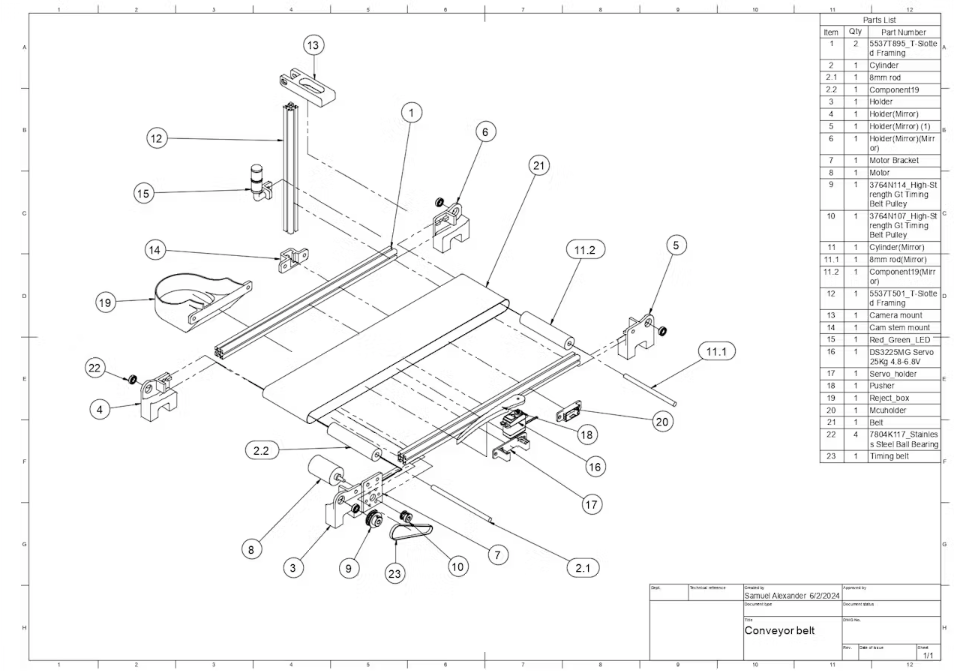
\includegraphics[width=0.7\textwidth]{images/prueba_de_concepto/planos_cinta.png}
   \caption[Planos de la cinta transportadora]{Planos de la cinta transportadora. Extraído de \cite{hackster_counting_inspection}.}
   \label{fig:planos_cinta}
\end{figure}

Los materiales empleados para la construcción de la cinta transportadora son los siguientes:

\begin{itemize}
   \item Un motor de corriente continua (DC) de 12V para el accionamiento de la cinta.
   \item Filamento PLA (ácido poliláctico) para la impresión 3D de las piezas estructurales de la cinta.
   \item Cuatro rodamientos de tipo 608ZZ para facilitar el movimiento suave de la cinta.
   \item Un servomotor de 9g, encargado de accionar el mecanismo de rechazo de canicas defectuosas.
   \item Una banda transportadora de 1.5 cm de ancho.
   \item Una placa microcontroladora Raspberry Pi Pico WH para el control del servomotor.
   \item Una cámara para la captura de imágenes de los objetos en la cinta.
   \item Cableado diverso y conectores para las interconexiones eléctricas.
   \item Una fuente de alimentación para suministrar energía a los componentes.
\end{itemize}

El montaje de la cinta transportadora se realizó siguiendo los planos ilustrados en la Figura \ref{fig:planos_cinta}. La Raspberry Pi Pico WH se programó para controlar el servomotor que desvía las canicas identificadas como defectuosas. Para la programación de este microcontrolador se utilizó MicroPython\cite{micropython_home}. La cámara se ubicó estratégicamente en la parte superior de la cinta para obtener una vista clara de las canicas durante su tránsito. El motor DC, alimentado por una fuente de 12V, es el responsable del movimiento continuo de la banda transportadora.

El sistema completo se configuró de la siguiente manera:
El procesamiento principal, incluyendo la ejecución del modelo de detección de objetos, se realiza en un dispositivo NVIDIA Jetson AGX Xavier. Este dispositivo es el encargado de analizar las imágenes capturadas por la cámara.
Para la comunicación entre el Jetson AGX Xavier y la Raspberry Pi Pico WH, se establece una conexión TCP/IP. Al iniciar el sistema, el Jetson AGX Xavier actúa como servidor, abriendo un socket en el puerto 5000 y esperando la conexión de la Raspberry Pi Pico WH (cliente).
Una vez que la Raspberry Pi Pico WH se conecta, envía un mensaje de inicio al Jetson. A partir de este momento, el Jetson comienza a procesar el flujo de vídeo de la cámara.
Cuando el modelo de detección en el Jetson identifica una canica defectuosa, envía un mensaje específico a la Raspberry Pi Pico WH.
Al recibir esta señal, la Raspberry Pi Pico WH activa el servomotor durante un breve instante. Este accionamiento mueve un mecanismo que desvía la canica defectuosa fuera de la trayectoria principal de la cinta transportadora.

%%%%%%%%%%%%%%%%%%%%%%%%%%%%%%%%%%%%%%%%%%%%%%%%%%%%%%%%%%%%%%%%%%%%%%%%%%%%%%%
%                                 CONCLUSIONS                                 %
%%%%%%%%%%%%%%%%%%%%%%%%%%%%%%%%%%%%%%%%%%%%%%%%%%%%%%%%%%%%%%%%%%%%%%%%%%%%%%%

\chapter{Conclusiones} \label{chap:conclusiones}

????? ????????????? ????????????? ????????????? ????????????? ?????????????

%%%%%%%%%%%%%%%%%%%%%%%%%%%%%%%%%%%%%%%%%%%%%%%%%%%%%%%%%%%%%%%%%%%%%%%%%%%%%%%
%                                BIBLIOGRAFIA                                 %
%%%%%%%%%%%%%%%%%%%%%%%%%%%%%%%%%%%%%%%%%%%%%%%%%%%%%%%%%%%%%%%%%%%%%%%%%%%%%%%

\printglossary[type=\acronymtype]

\bibliographystyle{plain}      % Estilo de la bibliografía
\bibliography{referencias} % Bibliografia

% \begin{thebibliography}{10}

% %%%%%%%%%%%%%%%%%%%%%%%%%%%%%%%%%%%%%%%%%%%%%%%%%%%%%%%%%%%%%%%%%%%%%%%%%%%%%%%
% % MODEL D'ARTICLE                                                             %
% %%%%%%%%%%%%%%%%%%%%%%%%%%%%%%%%%%%%%%%%%%%%%%%%%%%%%%%%%%%%%%%%%%%%%%%%%%%%%%%
% \bibitem{light}
%    Jennifer~S. Light.
%    \newblock When computers were women.
%    \newblock \textit{Technology and Culture}, 40:3:455--483, juliol, 1999.

% %%%%%%%%%%%%%%%%%%%%%%%%%%%%%%%%%%%%%%%%%%%%%%%%%%%%%%%%%%%%%%%%%%%%%%%%%%%%%%%
% % MODEL DE LLIBRE                                                             %
% %%%%%%%%%%%%%%%%%%%%%%%%%%%%%%%%%%%%%%%%%%%%%%%%%%%%%%%%%%%%%%%%%%%%%%%%%%%%%%%
% \bibitem{ifrah}
%    Georges Ifrah.
%    \newblock \textit{Historia universal de las cifras}.
%    \newblock Espasa Calpe, S.A., Madrid, sisena edició, 2008.

% %%%%%%%%%%%%%%%%%%%%%%%%%%%%%%%%%%%%%%%%%%%%%%%%%%%%%%%%%%%%%%%%%%%%%%%%%%%%%%%
% % MODEL D'URL                                                                 %
% %%%%%%%%%%%%%%%%%%%%%%%%%%%%%%%%%%%%%%%%%%%%%%%%%%%%%%%%%%%%%%%%%%%%%%%%%%%%%%%
% \bibitem{WAR}
% Comunicat de premsa del Departament de la Guerra, 
% emés el 16 de febrer de 1946. 
% \newblock Consultat a 
% \url{http://americanhistory.si.edu/comphist/pr1.pdf}.

% \end{thebibliography}
\cleardoublepage

%%%%%%%%%%%%%%%%%%%%%%%%%%%%%%%%%%%%%%%%%%%%%%%%%%%%%%%%%%%%%%%%%%%%%%%%%%%%%%%
%                           APÈNDIXS  (Si n'hi ha!)                           %
%%%%%%%%%%%%%%%%%%%%%%%%%%%%%%%%%%%%%%%%%%%%%%%%%%%%%%%%%%%%%%%%%%%%%%%%%%%%%%%

\APPENDIX

%%%%%%%%%%%%%%%%%%%%%%%%%%%%%%%%%%%%%%%%%%%%%%%%%%%%%%%%%%%%%%%%%%%%%%%%%%%%%%%
%                         LA CONFIGURACIO DEL SISTEMA                         %
%%%%%%%%%%%%%%%%%%%%%%%%%%%%%%%%%%%%%%%%%%%%%%%%%%%%%%%%%%%%%%%%%%%%%%%%%%%%%%%




% \chapter{Configuración del sistema} \label{ch:configuracion_sistema}

% ????? ????????????? ????????????? ????????????? ????????????? ?????????????

% \section{Fase de inicialización} \label{sec:fase_inicializacion}

% ????? ????????????? ????????????? ????????????? ????????????? ?????????????

% \section{Identificación de dispositivos} \label{sec:identificacion_dispositivos}

% ????? ????????????? ????????????? ????????????? ????????????? ?????????????

%%%%%%%%%%%%%%%%%%%%%%%%%%%%%%%%%%%%%%%%%%%%%%%%%%%%%%%%%%%%%%%%%%%%%%%%%%%%%%%
%                               ALTRES  APÈNDIXS                              %
%%%%%%%%%%%%%%%%%%%%%%%%%%%%%%%%%%%%%%%%%%%%%%%%%%%%%%%%%%%%%%%%%%%%%%%%%%%%%%%


\chapter{Objetivos de Desarrollo Sostenible} \label{ch:ods}

\begin{tabularx}{\textwidth}{|>{\raggedright\arraybackslash}X|c|c|c|c|}\hline
   \textbf{Objetivos de Desarrollo Sostenible} & \textbf{Alto} & \textbf{Medio} & \textbf{Bajo} & \textbf{No procede} \\ \hline
   ODS 1.  \textbf{Fin de la pobreza.}                            & & & & X \\ \hline
   ODS 2.  \textbf{Hambre cero.}                                  & & X & & \\ \hline
   ODS 3.  \textbf{Salud y bienestar.}                            & & & & X\\ \hline
   ODS 4.  \textbf{Educaci\'on de calidad.}                       & & & & X \\ \hline
   ODS 5.  \textbf{Igualdad de g\'enero.}                         & & & & X \\ \hline
   ODS 6.  \textbf{Agua limpia y saneamiento.}                    & & & & X \\ \hline
   ODS 7.  \textbf{Energ\'{\i}a asequible y no contaminante.}     & & & & X\\ \hline
   ODS 8.  \textbf{Trabajo decente y crecimiento econ\'omico.}    & X & & & \\ \hline
   ODS 9.  \textbf{Industria, innovaci\'on e infraestructuras.}   & X & & & \\ \hline
   ODS 10. \textbf{Reducci\'on de las desigualdades.}             & & & & X\\ \hline
   ODS 11. \textbf{Ciudades y comunidades sostenibles.}           & & & & X\\ \hline
   ODS 12. \textbf{Producci\'on y consumo responsables.}          & X & & & \\ \hline
   ODS 13. \textbf{Acci\'on por el clima.}                        & & & X & \\ \hline
   ODS 14. \textbf{Vida submarina.}                               & & & & X \\ \hline
   ODS 15. \textbf{Vida de ecosistemas terrestres.}               & & & & X\\ \hline
   ODS 16. \textbf{Paz, justicia e instituciones s\'olidas.}      & & & & X\\ \hline
   ODS 17. \textbf{Alianzas para lograr objetivos.}               & & & & X\\ \hline
   \end{tabularx}


   \section*{Justificación de los Objetivos de Desarrollo Sostenible} \label{sec:justificacion_ods}

   \textbf{ODS-8. Trabajo decente y crecimiento económico:} Este proyecto contribuye directamente al crecimiento económico sostenible mediante la automatización inteligente de procesos de control de calidad. La implementación de sistemas de detección de defectos basados en IA permite reducir costes operativos, minimizar desperdicios y optimizar la cadena de producción, lo que se traduce en mayor productividad y competitividad empresarial. Se alinea específicamente con la meta 8.2 de la ONU: «Lograr niveles más elevados de productividad económica mediante la diversificación, la modernización tecnológica y la innovación», al incorporar tecnologías avanzadas de procesamiento de imágenes y aprendizaje automático en entornos industriales tradicionales.

   \textbf{ODS-9. Industria, innovación e infraestructura:} El desarrollo de sistemas inteligentes para la detección de defectos representa una clara apuesta por la innovación industrial. Este proyecto no solo implementa tecnologías emergentes como la IA en procesos productivos, sino que además optimiza su rendimiento mediante el uso eficiente de hardware especializado como GPUs, algoritmos de seguimiento multi-objeto y técnicas de paralelización. Esto responde directamente a la meta 9.4 de la ONU: «Modernizar la infraestructura y reconvertir las industrias para que sean sostenibles, utilizando los recursos con mayor eficacia y promoviendo la adopción de tecnologías y procesos industriales limpios y ambientalmente racionales», al permitir mejoras significativas en eficiencia energética y uso de recursos mediante sistemas de inspección automatizados.

   \textbf{ODS-12. Producción y consumo responsables:} La implementación de sistemas de detección temprana de defectos contribuye sustancialmente a la producción responsable mediante: 1) la reducción del descarte de productos y materias primas al identificar problemas en etapas iniciales del proceso productivo, 2) la optimización del consumo energético al evitar el procesamiento completo de productos defectuosos, y 3) la mejora de la calidad final que aumenta la vida útil de los productos. Estas aportaciones se vinculan directamente con la meta 12.5 de la ONU: «De aquí a 2030, reducir considerablemente la generación de desechos mediante actividades de prevención, reducción, reciclado y reutilización», ya que el sistema desarrollado actúa preventivamente evitando la generación de residuos industriales y facilitando la reutilización de materiales recuperados.

%%%%%%%%%%%%%%%%%%%%%%%%%%%%%%%%%%%%%%%%%%%%%%%%%%%%%%%%%%%%%%%%%%%%%%%%%%%%%%%
%                              FI DEL DOCUMENT                                %
%%%%%%%%%%%%%%%%%%%%%%%%%%%%%%%%%%%%%%%%%%%%%%%%%%%%%%%%%%%%%%%%%%%%%%%%%%%%%%%
\printglossaries

\end{document}